%!TEX root = ../../dissertation.tex
%%%%%%%%%%%%%%%%%%%%%%%%%%%%%%%%%%%%%%%%%%%%%%%%%%%%%%%%%%%%%%%%%%%%%%%%%%%%%%%%
\chapter{Mobile Core Network Investigation}
\label{chap:mobilenets}

The rise of reliable video streaming is not happening completely independent of other developments. Instead, it is deeply embedded into major shifts in Internet access. With more and more smartphones being used and even dial-up Internet access sometimes being replaced with stationary mobile \gls{3G} and \gls{LTE} modems. All these ``over-the-top'' streaming services are now being used within mobile networks.

Today's cellular mobile networks are usually based on \gls{3GPP} specifications which have evolved from the circuit switched \gls{GSM} network into the fully packet switched \gls{LTE} which is still in its unrolling phase. But simply being packet switched does not mean that it shares a lot of similarity with a typical wireline \gls{IP} stack and network access infrastructure, for example a \gls{VDSL} or \gls{DOCSIS} dial-up connected to an \gls{IP} network. 

A \gls{3G} network (a term synonymous for the typical combined \gls{GSM} and \gls{UMTS} cellular network in use today) is very distinct from typical wired networks as it provides, amongst others, mobility and authentication in its lower layers through the core specifications rather than being optional on-top services as is typically the case in the Internet. To achieve this, large amounts of state have to be kept at each network node and is explicitly communicated among the network nodes in its \gls{CN}. Also, the lines separating layers and functions are very blurred, making it very hard to grasp parts of the architecture without understanding the whole. Many specialized protocols are involved to communicate intents and states in the network. This causes processing overhead and signaling traffic on the network paths on top of the actually useful user traffic. 

It is a known fact, that radio spectral resources are a scarce resource that need to be well managed. But it might not seem immediately obvious to think the same about control plane resources in the infrastructure of a mobile network. Yet, there have been accounts\footnote{``Docomo Counts Cost of Signaling Storm'',\url{http://www.lightreading.com/d/d-id/693779}}\footnote{``Android Signaling Storm Rises in Japan'', \url{http://www.lightreading.com/a/d-id/693138}}\footnote{``Angry Birds + Android + ads = network overload'', \url{http://www.itwire.com/business-it-news/47823}} (\cite{huawei2011storm}) of situations where the core network has been flooded with signaling, despite only a negligible amount of actual user traffic being transported. This resulted in an event dubbed ``signaling storm'', causing an unintentional \gls{DDoS} attack, disrupting user-plane connectivity on its way.

The state of research on the architecture and especially the control plane behavior of \gls{3G} mobile cellular networks is lean in comparison to the huge volume of research conducted other wired Internet structures. Most of the available research focuses on user-oriented metrics such as traffic statistics and mobility patterns, or only investigates properties of the radio interface. Little has been published about activity within the core network, and yet less about core signaling. 

Conducting \gls{IP} traffic research at the network's edge, independent of the access technology, is usually relatively easy. Writing simple tests and measurement scripts, that record the user's traffic, is all that is needed. But mobile phones do not allow one to peek inside its layer 1 and 2 implementation and interaction, where the control plane resides. Any information on this black box can only be indirectly inferred from layers above --- by forcing behavior known from specification --- or below --- through spectrum analysis using \gls{SDR} approaches. 

However, to directly investigate the core as well as the control plane, some kind of a measurement infrastructure inside the network is needed. With this, researchers could not just look into user traffic flowing through the network but also investigate the signaling heavy mobile network control plane. But to gain this kind of access to the network  would require the cooperation of a mobile network operator, which they grant very reluctantly due to privacy and competitive concerns.

Another important aspect related to signaling is network dimensioning. Operators mostly dimension their networks in accordance to the expected user traffic. But in such a signaling-dependent architecture this might not be the most fitting approach, as the mentioned signaling storms seem to demonstrate. 

This chapter attempts to remedy parts of the problem. Data from an existing mobile network measurement infrastructure is used to evaluate aspects of the control plane. 

Section~\ref{c4:sec:3gpparchitecture} discusses the required details of the mobile network architecture under investigation followed by a survey of existing literature in Section~\ref{c4:sec:relwork}. Next, an attempt on defining and inferring control plane load is made in Section~\ref{c4:sec:loaddefinition}. This is used to find viable targets for a potential load evaluation. 

Further methodology is given in Section~\ref{c4:sec:methodology} with the actual evaluation including a statistical analysis to follow in Section~\ref{c4:sec:evaluations}. The measurement data backs up a number of assumptions on the behavior of different device and operating system types, but also reveals some remarkable differences in signaling characteristics. Afterwards, the evaluation results are used to construct load models for the current \gls{CN} in Section~\ref{c4:sec:modeling}. This is extended with possible modifications to it and a numerical simulation to confirm the model viability.


%%%%%%%%%%%%%%%%%%%%%%%%%%%%%%%%%%%%%%%%%%%%%%%%%%%%%%%%%%%%%%%%%%%%%%%%%%%%%%%
%!TEX root = ../../dissertation.tex
%%%%%%%%%%%%%%%%%%%%%%%%%%%%%%%%%%%%%%%%%%%%%%%%%%%%%%%%%%%%%%%%%%%%%%%%%%%%%%%%
\section{Core Architecture Overview}
\label{c4:sec:3gpparchitecture}

Today's dominating commercial mobile network system, which combines \gls{GSM}, \gls{UMTS}, and now often also \gls{LTE}, is designed and specified by the \gls{3GPP}. This group is an umbrella organization for several standardization bodies, including the European \gls{ETSI} and their individual members --- in this case mostly telecommunication companies. Unlike the \gls{IETF}, the Internet's de facto standards body, natural persons cannot participate in the \gls{3GPP} on their own but only through the organizational members.

Specifications are not released individually but are instead grouped together into larger releases once every or every other year. \gls{GSM} was first specified in the \textit{Phase 1} release in 1992 with \gls{GPRS} added in \textit{Release 97} (1998). \gls{UMTS} followed with \textit{Release 99} (2000), but most \gls{3G} networks operate at least with \textit{Release 5} (2002), \textit{Release 6} (2004), or \textit{Release 7} (2007) as they introduced \gls{HSDPA}, \gls{HSUPA}, and \gls{HSPA+} likewise. \gls{LTE} first found its way into the specifications in 2008 with \textit{Release 8}. \textit{Release 12} is scheduled to be published in March of 2015. This background section mostly describes the \gls{UMTS} based \gls{TS} with some comparisons being made to the older \gls{GPRS} and the latest \gls{LTE} specification versions where available.

\begin{figure}[htbp]
	\centering
	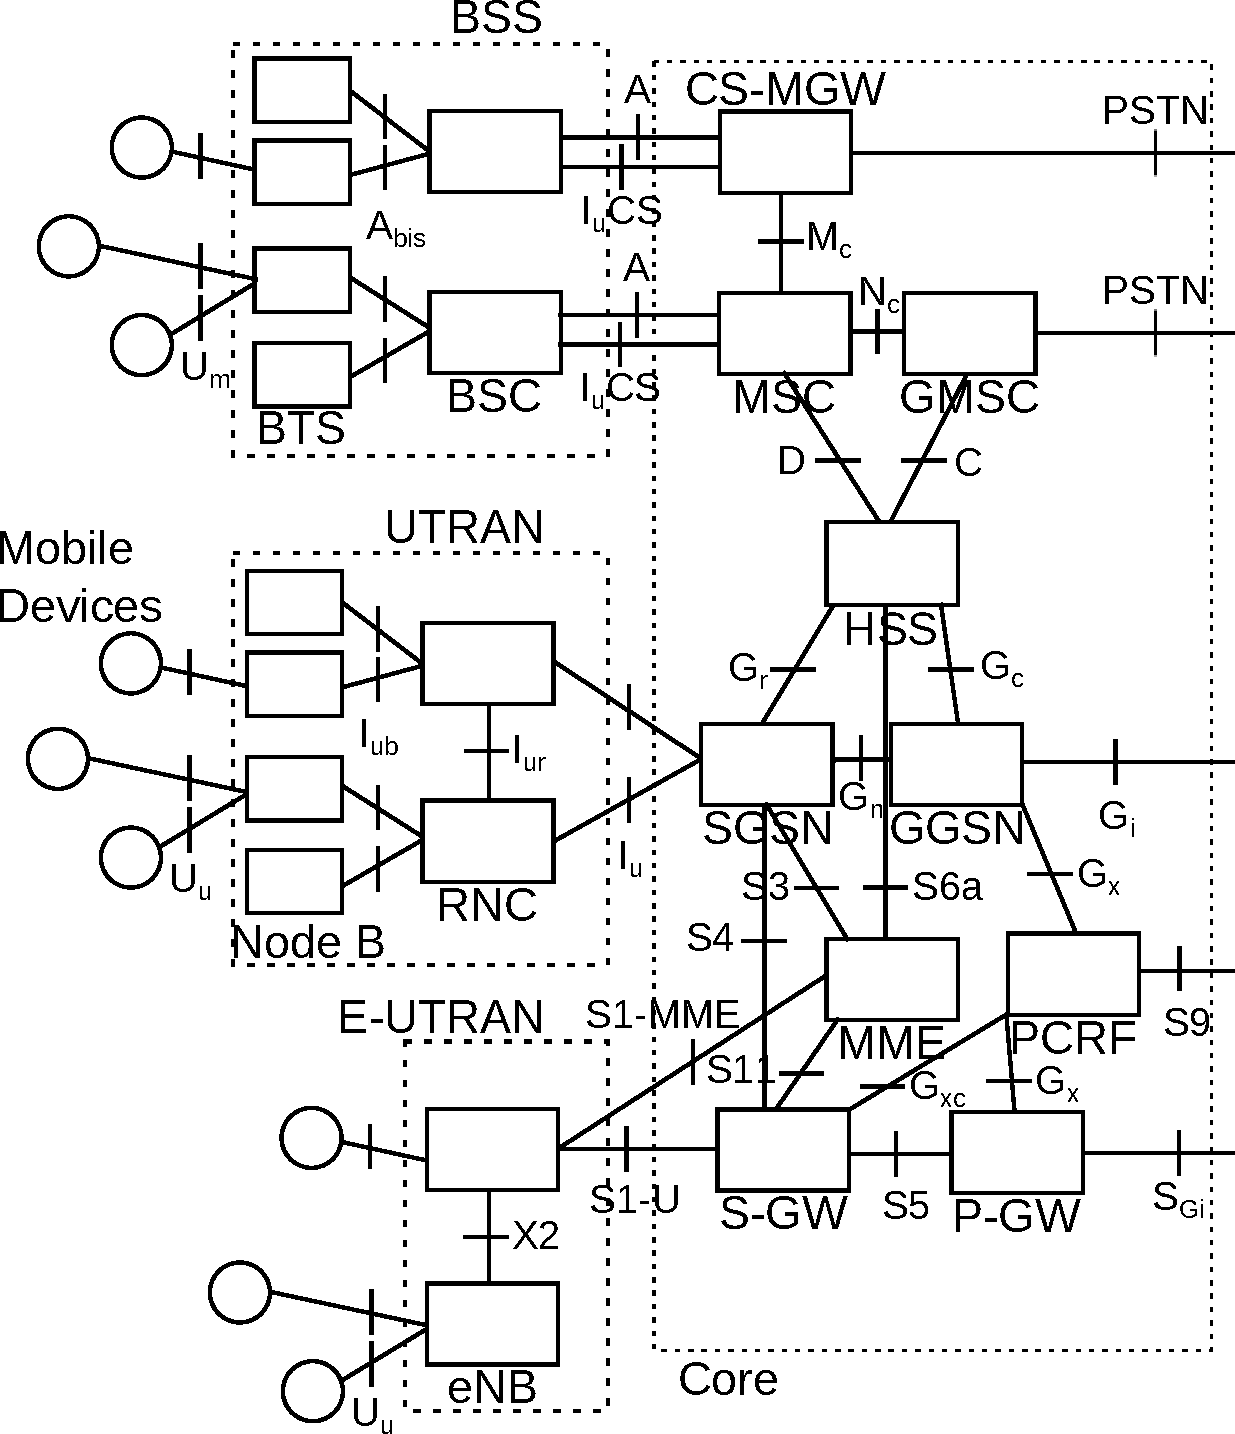
\includegraphics[width=1.0\textwidth]{images/3gpp-physical-arch.pdf}
	\caption{Overview of a combined \acrshort{CS}/\acrshort{PS} \acrshort{GSM}/\acrshort{UMTS}/\acrshort{LTE} architecture.}
\label{c4:fig:psdomain}
\end{figure}

Today's most common version of the mobile network architecture is depicted in Figure~\ref{c4:fig:psdomain} and based on \gls{3GPP} \gls{TS} 23.002~\cite{3gpp.23.002}, with some minor nodes and network paths omitted\footnote{For a complete reference of all the acronyms and addressing schemes used in \gls{3GPP} specs please refer to \gls{TS} 21.905~\cite{3gpp.21.905} and \gls{TS} 23.003~\cite{3gpp.23.003}}. The displayed architecture combines all three access technologies as well as the \gls{CS} and the \gls{PS} domains of the core. 

Concerning the \gls{PS} domain, one has to further distinguish between links and nodes used solely for control plane tasks as well as links and nodes that are in path of the actual user \gls{IP} traffic. For \gls{UMTS} and \gls{GPRS}\footnote{\gls{GPRS} provides \gls{PS} data services for \gls{GSM} radio access. The same core infrastructure is also used in the \gls{UMTS} \gls{PS} domain.} the \gls{SGSN} and the \gls{GGSN} are the core elements inside the user traffic path. Everything else solves just control plane tasks.

One thing to keep in mind is the strict separation between user plane and control plane tasks in the \gls{3GPP} architecture. Here completely separate protocol stacks are used and signaling is mostly conducted in an explicit and out of band manner. This is contrary to the typical approach of the Internet's \gls{TCP}/\gls{IP} stack, especially its upper layers, where most state is implicitly inferred and only some signaled in-band. 

The following sections give a short description of nodes and their tasks as well as used protocols stacks and signaling procedures for both the user and the control plane. The description will be mostly focused on the \gls{UMTS} parts of the architecture which is also overviewed in \cite{3gpp.23.101}.


%%
\subsection{\texorpdfstring{\acrshort{3GPP}}{3GPP} Radio Network}

The architecture has three completely distinct radio networks, one for each access technology: \gls{GSM}'s \gls{BSS} (or more complete: \gls{GERAN}), \gls{UTRAN} for \gls{UMTS}, and \gls{E-UTRAN} in \gls{LTE}.

Essential to the radio network is a base station, a radio transceiver providing the physical connection to the user's mobile device\footnote{Mobile devices are called \gls{MS} in \gls{GSM} networks and \gls{UE} in \gls{3G} and later.} \gls{3G}'s base station is called \textit{Node B}. The used radio spectrum is divided into a number of channels, with various shared channels responsible for management and control plane signaling and one or more dedicated channel for each active mobile device~\cite{3gpp.25.201,3gpp.25.301}. Layer 2 consists of several protocols managing and multiplexing transmissions on the link. These are \gls{MAC}~\cite{3gpp.25.321} and \gls{RLC}~\cite{3gpp.25.322} with an additional user plane broadcast service provided by \gls{BMC}~\cite{3gpp.25.324}. 

On layer 3, the actual radio control plane signaling protocol \gls{RRC} \cite{3gpp.25.331} resides, managing the device's state and the radio connection. Some of the signaling procedures are detailed in \cite{3gpp.25.931}. Additionally, \gls{PDCP}~\cite{3gpp.25.323} provides the connection to the  usual Internet \gls{TCP}/\gls{IP} user plane stack atop. Thus, all user traffic is encapsulated into so called \textit{radio bearers}, which tunnels traffic from the mobile device directly into the core network.

Each base station acts as an independent radio cell. Mobile devices can be seamlessly handed over between cells without higher layers being able to notice this.\footnote{However, there are still many ways to detect a handover in the upper layers of a mobile device.} The handover process is fully controlled and conducted by the network through a node that shares the old and new path to the device. For \gls{UMTS}, in most cases this can be handled by the \gls{RNC} while the core \gls{SGSN} is responsible for handovers between larger regions.

In \gls{UMTS} multiple base stations are concentrated into one \gls{RNC}. Most of the functions of a \gls{RNC}, including \gls{MM}, are defined by the \gls{RANAP} control plane protocol defined in \cite{3gpp.25.413}. \gls{RANAP} is used at the Iu interface between the \gls{RNC} and the core network, i.e., the \gls{SGSN}. Today, all non-radio links of the network are usually \gls{IP}-based. But in the past all interfaces have also been explicitly defined for \gls{ATM} and exhibited some differences to their \gls{IP}-based counterparts. The connection of the decentralized parts of the radio network to either the core network itself or a \gls{RNC} is called \textit{backhaul}. This term usually subsumes the bulk transport of data over dedicated links to a central location. Often, optical fiber or microwave transmission links are used.


%%
\subsection{\texorpdfstring{\acrshort{3GPP}}{3GPP} Core Network}

The \gls{PS} domain of a mobile core network manages most of the aspects of the connected devices and acts as the bridge and gateway to the Internet. It consists of nodes that are directly in the path of the user plane traffic as well as additional nodes, that only exist in the control plane.

\gls{GPRS} and \gls{UMTS} use the exact same \gls{PS} core network architecture. Only \gls{LTE} introduced a new core network concept, the \gls{EPC}. If one core has to simultaneously provide support for both \gls{UMTS} and \gls{LTE} access, core nodes for both architectures have to be present. The exception are some \gls{EPC} nodes that provide legacy interfaces to supplant their \gls{UMTS} predecessors.

The two central elements in the user plane's path are the \gls{SGSN} and the \gls{GGSN}~\cite{3gpp.22.060,3gpp.23.060}. The \gls{SGSN} is the endpoint of the \gls{RAB}, tunneling user traffic from the \gls{UE} to the core, and an endpoint for the \gls{gtp} based core tunnel, further transporting user plane traffic to the \gls{GGSN}. \Gls{gtp} will be described in detail in Section~\ref{c4:sec:gtp}. The \gls{GGSN}'s control plane tasks include mobility and connection management via \gls{RANAP} to the \gls{RNC}. The necessary information is cached and retrieved from the \gls{HLR} using \gls{MAP}~\cite{3gpp.29.002}. The \gls{HLR} or, respectively, the \gls{HSS} in an \gls{EPC}, acts as the central storage of all the operator's subscriber information.

The \gls{GGSN} represents the gateway to the public Internet and therefore typically is the only node in the network, that has a publicly routable \gls{IP} address. It filters incoming traffic into the corresponding \gls{gtp} tunnel and routes packets to the correct \gls{SGSN}. State about any active tunnel and device has to be kept locally and is initially retrieved from the \gls{SGSN}.

In \gls{EPC} user traffic in the core is handled by the \gls{SGW} and \gls{PGW}, having similar functions as their \gls{GPRS} counterparts \gls{SGSN} and \gls{GGSN}. Depending on the specific version of the implemented infrastructure these two nodes can also be combined into one, eliminating the S5 interface and the \gls{gtp} signaling between them. Much of the control plane tasks of the \gls{SGSN} have now been offloaded to a new node, the \gls{MME}, which maintains its own logical connection to the radio network using the \gls{S1AP} signaling protocol~\cite{3gpp.36.413}. Instead of \gls{MAP} to retrieve user data from the central storage, Diameter~\cite{rfc6733} is now used to communicate with the \gls{HSS}. Of note is also a further addition to the \gls{EPS}: the \gls{PCRF} in conjunction with the \gls{PCEF} which is integrated into the \gls{PGW}. They act as a \gls{DPI} entity, inspecting all user plane traffic and enable arbitrary filtering of traffic and traffic-based billing. Both entities are described in \cite{3gpp.23.203}.

\begin{figure}[htbp]
	\centering
	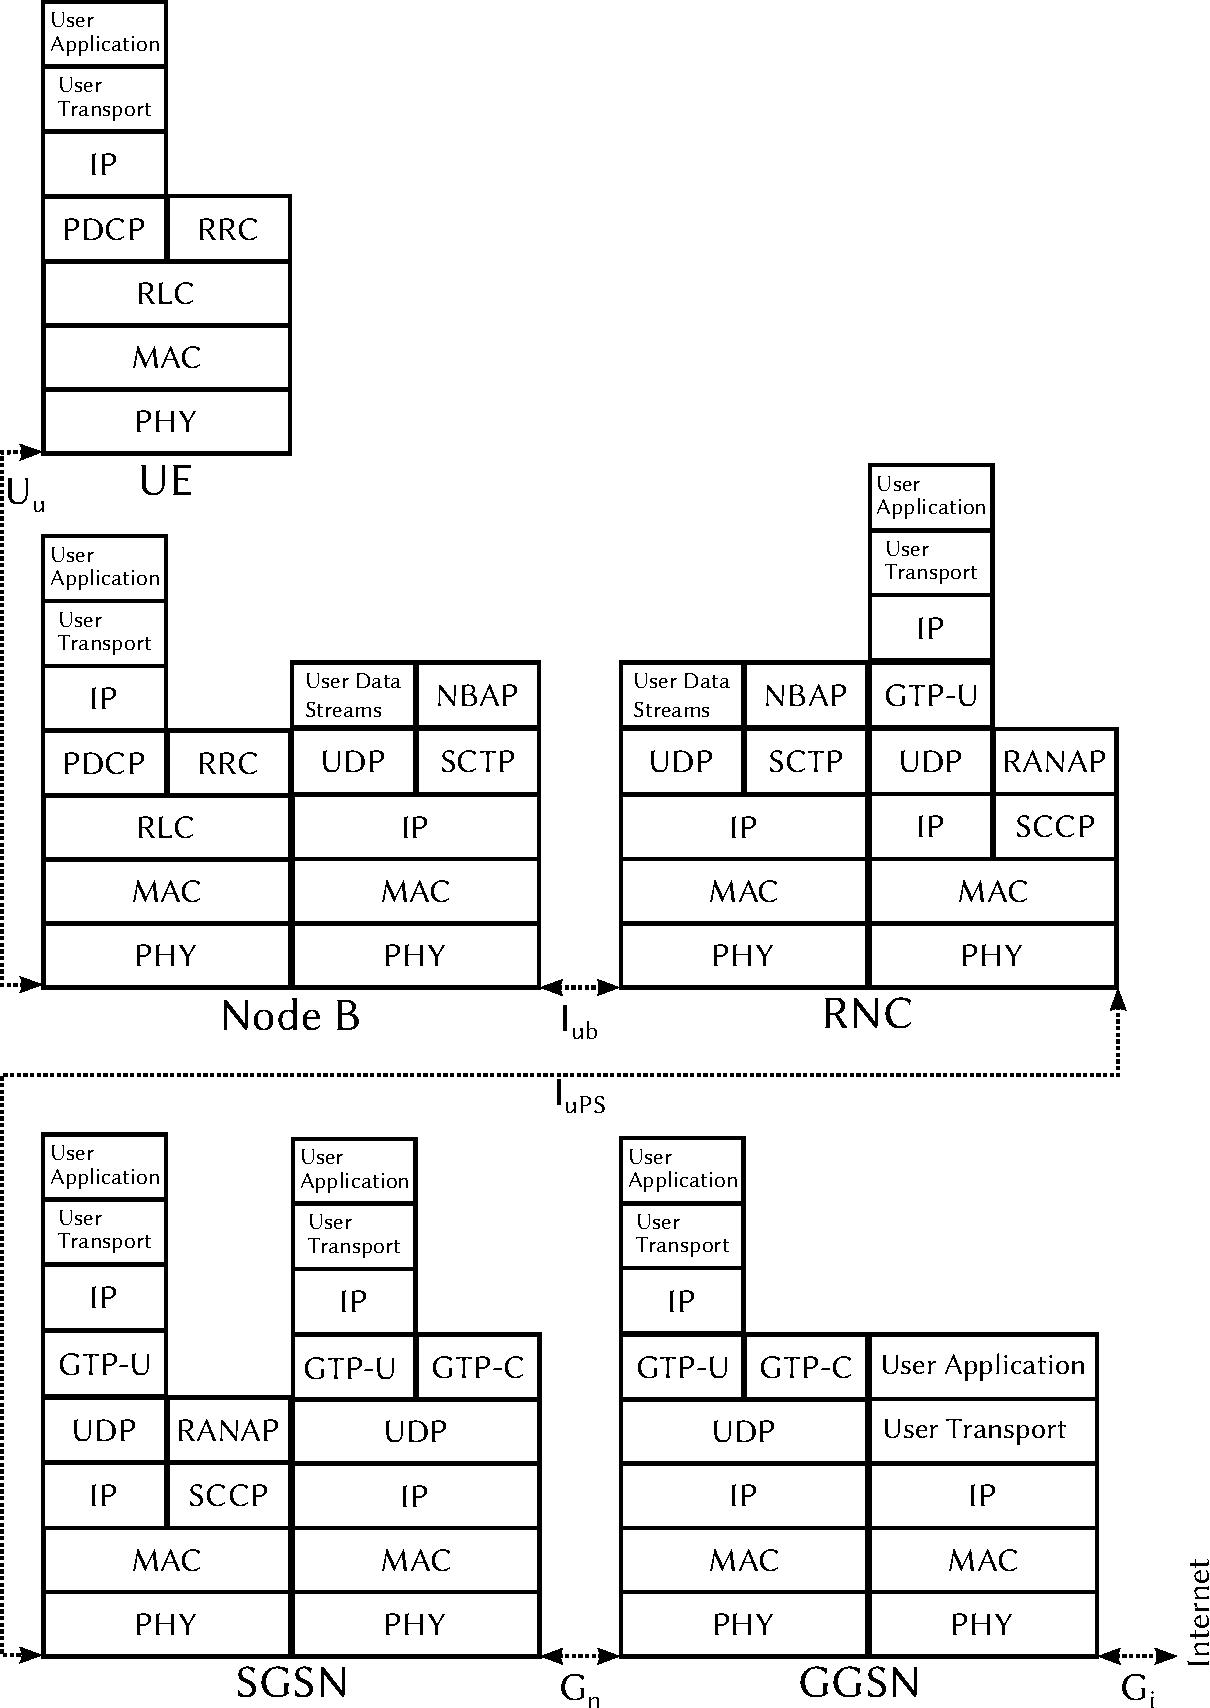
\includegraphics[width=0.9\textwidth]{images/umts-userpath-stack.pdf}
	\caption{Simplified control plane and user plane \acrshort{IP}-based protocol stacks on the user traffic path through the mobile network.}
\label{c4:fig:protocolstacks}
\end{figure}

Figure~\ref{c4:fig:protocolstacks} overviews the complete protocol stack on the path of the user traffic through the whole network from the \gls{UE} to an external network.


%%
\subsection{Core Network Concepts}

Most of the discussed upcoming research deals with the core network. Therefore, this next sections will explain in detail the concepts behind the \gls{3G} core network control plane and the \gls{gtp} protocol family.

As mentioned, there is a strict separation between control instances and instances that carry the actual user traffic. Looking at the control plane side of things, management is conducted in a completely stateful way. Nodes keep track of every \gls{UE} they are managing and need to locally store any state information they might need for management purposes. Of particular interest is the state revolving around the \textit{\gls{PDP} Context}. For each open data connection a device has, both the \gls{GGSN} and \gls{SGSN} must keep such a \gls{PDP} Context, which identifies the connection as well as the device belonging to it.

Additionally, a number of state machines are maintained. Transitions between machine states trigger a signaling message to specific network neighbors. Any one of these signaling interactions belongs to one or more larger control plane procedures. Most of the procedures that happen inside the core network \gls{PS} domain or affect it are defined in \gls{TS}~24.008~\cite{3gpp.24.008} and \gls{TS}~23.060~\cite{3gpp.23.060}.

\begin{figure}[htbp]
	\centering
	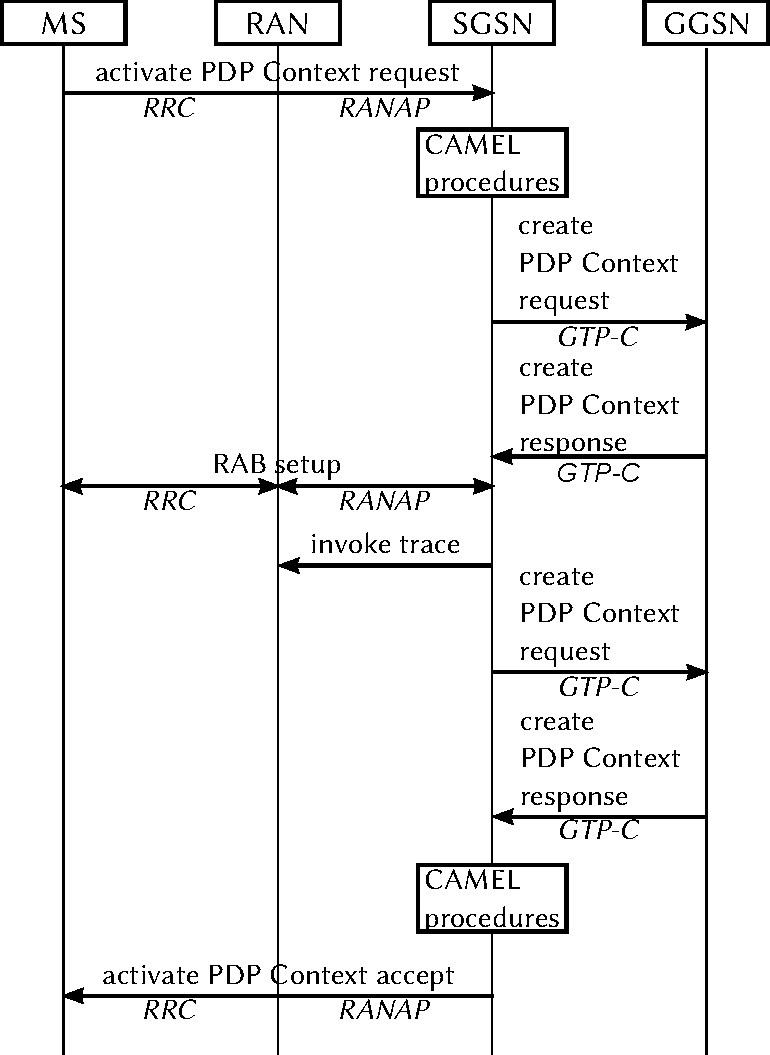
\includegraphics[width=0.7\textwidth]{images/pdp-context-activation-procedure.pdf}
	\caption{\acrshort{PDP} Context activation procedure signaling interaction diagram for \acrshort{UMTS}, including involved signaling protocols.}
\label{c4:fig:pdpcontextactivationinteraction}
\end{figure}

A very simple example is demonstrated in Figure~\ref{c4:fig:pdpcontextactivationinteraction}. Initiated by the \gls{UE}'s session management state machine a data connection to the device is requested to be set up, triggering signaling with various protocols throughout the network. Additional secondary \gls{CAMEL} procedures, defined in \cite{3gpp.23.078}, are also triggered and conducted.

The general motif of control in \gls{3G} networks is rather different to that of the typical \gls{TCP}/\gls{IP} Internet stack. Whereas plain \gls{IP} stacks rely on the end-to-end principle and put most of the control inside the devices at the edge, in \gls{3G} control procedures are spread across the network. Coordinating this requires the discussed control plane and all of the explicit signaling interactions. This results in a rather high complexity but also gives the opportunity to investigate these mechanisms and implications the structures have on the performance.


%%
\subsection{Tunneling Concept: Bearers and \texorpdfstring{\acrshort{PDP}}{PDP} Contexts}

To enact the aforementioned user and control plane separation, a custom tunneling concept is used. Beginning at the \gls{UE}, the actual user \gls{IP} stack is never directly carried over the link's layer 1 and 2 protocols but always further encapsulated into so called \textit{bearer}. The specifications distinguish between the \textit{radio bearer} on the air interface, the \gls{RAB} denominates the path between the \gls{UE} and the \gls{CN}, where it is called \gls{CN} bearer.

Technically, different protocols with tunneling capability are used on each link. \gls{PDCP} is used on the radio link, \gls{GTP-U} is employed between the \gls{RAN} and the \gls{CN} and in the core between \gls{SGSN} and \gls{GGSN}. Closely related to the core network bearer are a number of information records stored and maintained at the two core nodes, the aforementioned \gls{PDP} Context. For every active bearer a context is stored containing identification and management information about it. Amongst others this includes device identifiers, e.g., \gls{IMSI} and \gls{IMEI}, tunnel identifiers (\gls{TEID}), information about the intended public network through the \gls{APN} field, charging, and \gls{QoS} \cite[Section~13]{3gpp.23.060}.

Commonly, any device with an active data connection has at least one bearer and an associated \gls{PDP} Context, the \textit{default bearer}. In terms of \gls{QoS} this represents a best effort tunnel carrying all user traffic that is not further differentiated. Additionally, the device can request a number of secondary tunnels, i.e., \textit{dedicated bearers}, with certain \gls{QoS} guarantees. Traffic matching a specified \gls{TFT} will then be carried over this dedicated bearer. However, this concept is scarcely used in \gls{3G} networks. All in all, one \gls{UE} can be associated with up to eleven bearers, consisting of one default bearer and additional dedicated bearers.


%%
\subsection{\texorpdfstring{\acrshort{gtp}}{GTP} and \texorpdfstring{\acrshort{gtp}}{GTP}-based Core Network Signaling}
\label{c4:sec:gtp}

A large part of core network communication is conducted by \gls{gtp}. In \gls{3G} networks version 1 of the protocol is used and defined in \gls{TS}~29.060~\cite{3gpp.29.060} and \gls{TS}~29.281~\cite{3gpp.29.281}.\footnote{For a more concise description of the protocol, one should actually read the \gls{gtp} implementation in the community \gls{FOSS} project OpenGGSN at \url{https://github.com/osmobuntu/openggsn}.} For \gls{EPC} some changes were made to \gls{gtp} bringing it to version 2, which is specified in \gls{TS}~29.274~\cite{3gpp.29.274}. The latter will not be further discussed as all presented evaluations will have a \gls{3G} network as basis.

\gls{gtp} is mainly used on the Gn interface that connects the two main \gls{GPRS} nodes, the \gls{GGSN} and \gls{SGSN}. Its functionality is split up between a user plane and a control plane part, named respectively \gls{GTP-U} and \gls{GTP-C}. \gls{gtp} can best be described as an application layer signaling protocol and is intended to be transported by \gls{UDP}.

\begin{figure}[htb]
	\begin{tabu}{X[1]|X[1]|X[1]|X[1]|X[1]|X[1]|X[1]|X[1]|X[1]|}
	\multicolumn{1}{c}{} & \multicolumn{8}{c}{\textbf{Bits}} \\
	\textbf{Octets} & \textbf{8} & \textbf{7} & \textbf{6} & \textbf{5} & \textbf{4} & \textbf{3} & \textbf{2} & \textbf{1} \\ 
	\cline{2-9} \textbf{1} & \multicolumn{3}{c|}{Version}  & 1 & 0 & E & S & PN \\ 
	\cline{2-9} \textbf{2} & \multicolumn{8}{c|}{Message Type}  \\ 
	\cline{2-9} \textbf{3} & \multicolumn{8}{c|}{\multirow{2}{*}{Length}}  \\ 
				\textbf{4} & \multicolumn{8}{c|}{}  \\ 
	\cline{2-9} \textbf{5} & \multicolumn{8}{c|}{\multirow{4}{*}{Tunnel Endpoint Identifier}} \\ 
				\textbf{6} & \multicolumn{8}{c|}{} \\ 
				\textbf{7} & \multicolumn{8}{c|}{} \\ 
				\textbf{8} & \multicolumn{8}{c|}{} \\ 
	\cline{2-9} \textbf{9} & \multicolumn{8}{c|}{\multirow{2}{*}{Sequence Number}} \\
				\textbf{10} & \multicolumn{8}{c|}{} \\
	\cline{2-9}	\textbf{11} & \multicolumn{8}{c|}{N-PDU} \\
	\cline{2-9} \textbf{12} & \multicolumn{8}{c|}{Next Extension Header Type} \\
	\cline{2-9}
	\end{tabu} 
	\caption{General \SI{12}{\byte} \acrshort{gtp} header format.}
\label{c4:fig:gtpheader}
\end{figure}

Conceptually, \gls{gtp} is structured through a base packet header, a number of extension headers and a message body consisting of a series of \gls{IE}. The base header is depicted in Figure~\ref{c4:fig:gtpheader} and has a total length of \SI{12}{\byte}. Essential to the header are the \gls{TEID} to identify the corresponding user plane tunnel and the \SI{8}{\bit} message type field. Each of the message types corresponds to a specific signaling interaction from the overarching control plane procedures. The procedures that \gls{gtp} concerns itself with on the Gn path belong either to path management, tunnel management, or mobility management. Messages also usually come in request and response pairs which must be sent from the receiving node back to the original requester.

Each messages is defined as a specific set of \glspl{IE}, each of which is either mandatory, conditional to some external factor, or optional. These \gls{IE}, depending on the type either of fixed or variable length, convey the actual state to be signaled and always relate to a specific \gls{UE} and tunnel, for example the device's \gls{IMSI} or the configured \gls{APN}.

\begin{table}[htbp]
\caption{All \acrshort{IE} in a Create \acrshort{PDP} Context request and size thereof for \acrshort{IPv4} network and user traffic only. The denoted sizes exclude the first message type byte.}
\label{c4:tab:createrequestelements}
	\begin{tabu} to 0.49\textwidth{X[2.5]X[1.2]X[0.7]}
		\toprule
		\textbf{\gls{IE}} & \textbf{Presence} & \textbf{Size}\\
		\midrule
		\gls{IMSI} & cond. & \SI{8}{\byte} \\ 
		\acrshort{RAI} & opt. & \SI{6}{\byte} \\
		Recovery & opt. & \SI{1}{\byte} \\
		Selection mode	& cond. & \SI{1}{\byte} \\
		\gls{TEID} Data I & mand. & \SI{4}{\byte} \\
		\gls{TEID} Control Plane & cond. & \SI{4}{\byte} \\
		\gls{NSAPI} & mand. & \SI{1}{\byte} \\
		Linked \gls{NSAPI} & cond. & \SI{1}{\byte} \\
		Charging Characteristics & cond. & \SI{2}{\byte} \\
		Trace Reference & opt. & \SI{2}{\byte} \\
		Trace Type & opt. & \SI{2}{\byte} \\
		End User Address & cond. & \SI{8}{\byte} \\
		\gls{APN} & cond. & max \SI{102}{\byte} \\ % APN format defined in 23.003 section 9
		\acrshort{PCO} & opt. & max \SI{255}{\byte} \\ % defined in 24.008 section 10.5.6.3
		\gls{SGSN} signaling address & mand.  & \SI{6}{\byte} \\ % defined in 23.003 section 5 (without address type and length fields)
		\gls{SGSN} user traffic address & mand. & \SI{6}{\byte} \\ % same as above
		\gls{MSISDN} & cond. & max \SI{17}{\byte} \\ % ITU-T E.164 msisdn format recommendation of max 15 chars
		\gls{QoS} Profile & mand. & max \SI{257}{\byte} \\
		\bottomrule
	\end{tabu}%
	\raisebox{0.95mm}{\begin{tabu} to 0.49\textwidth{X[2.5]X[1.2]X[0.7]}
		\toprule
		\textbf{\gls{IE}} & \textbf{Presence} & \textbf{Size} \\
		\midrule
		\gls{TFT} & cond. & max \SI{257}{\byte} \\ % defined in 24.008 section 10.5.6.12
		Trigger Id & opt. & var. \\ % no definition found
		\acrshort{OMC} Identity & opt. & var. \\ % maybe in MAP 29.002, however not further definition found
		Common Flags & opt. & \SI{3}{\byte} \\
		\gls{APN} Restriction & opt. & \SI{3}{\byte} \\
		\gls{RAT} & opt. & \SI{3}{\byte} \\
		User Location Information & opt. & \SI{10}{\byte} \\
		\gls{MS} Time Zone & opt. & \SI{4}{\byte} \\
		\gls{IMEI} (\acrshort{SV}) & cond. & \SI{10}{\byte} \\
		\gls{CAMEL} Charging Information Container & opt. & var. \\
		Additional Trace Info & opt. & \SI{11}{\byte} \\
		Correlation-ID & opt. & \SI{3}{\byte} \\
		Evolved Allocation Retention Priority I & opt. & \SI{3}{\byte} \\
		Extended Common Flags & opt. & \SI{3}{\byte} \\ % might be more, but seems unused 
		User \acrshort{CSG} Information & opt. & \SI{10}{\byte} \\
		\gls{APN}-\acrshort{AMBR} & opt.  & \SI{11}{\byte} \\
		Signaling Priority Indication & opt. & \SI{3}{\byte} \\ % might be more, but seems unused
		Private Extension & opt. & var. \\
		\bottomrule
	\end{tabu}}
	%\vfill
	%\null
\end{table}

Coming back to the described \gls{PDP} Context activation procedure, it contains both the \gls{gtp} message \textit{Create \gls{PDP} Context request} as well as the \textit{response} twice. Such a Create request consists of the 36 \gls{IE} depicted in Table~\ref{c4:tab:createrequestelements}. Neglecting the elements which have no predefined upper length bound (besides the default \SI{16}{\bit} \gls{IE} length field) and assuming a maximum length for the other variable elements this results in a message size of \SI{1059}{\byte}. The complexity of the other message types is comparable.

One of the investigations that will be conducted is that of the core network load, which will be defined and discussed later in detail. \gls{gtp} messages could play an interesting role here as they may directly or indirectly contribute to this load or at least be an indicator of load existing otherwise. Load could be caused by the generated network traffic as well as the assembly, processing, and storage of the involved state in form of the \gls{IE}.

The following sections detail the three \gls{gtp} tunnel management message pairs involved in the maintenance of \gls{PDP} Contexts. These are the \textit{Create, Update,} and \textit{Delete \gls{PDP} Context requests} and \textit{responses}. They represent the basis for the core network investigations.


%%
\subsubsection{Create \gls{PDP} Context Message}

This message type is part of procedures that enable the \gls{PS} data connection and the \gls{gtp} tunnel for a mobile device. These are the \textbf{\gls{PDP} Context activation procedure} (already depicted in Figure~\ref{c4:fig:pdpcontextactivationinteraction}) and the \textbf{Secondary \gls{PDP} Context activation} for additional \gls{gtp} tunnels to the device with specific \gls{QoS} levels set. They are triggered by the mobile device through \gls{RRC}/\gls{RANAP} signaling during or following a \gls{GPRS} attach procedure.

When a \gls{GGSN} receives a create request from an \gls{SGSN}, it has to allocate the necessary resources for a \gls{PDP} Context. Depending on the outcome, a response is sent back, indicating the success or failure of the operation. Typical failures include failed user authentication, a lack of resource, or unrecoverable system failures and malformed or corrupted request.


%%
\subsubsection{Delete \gls{PDP} Context Message}

Similar to to Create Context messages, a \textbf{Delete \gls{PDP} Context request} and \textbf{response} always coincides with the termination of a \gls{gtp} tunnel and the removal of the associated \gls{PDP} Context. Together, these mark the beginning and the end of every user traffic tunnel, making them very interesting in determining tunnel properties and perfect candidates to indirectly identify tunnel durations in a core network investigation.

Deletes are either created through explicit \gls{PDP} Context deactivation procedures or play a part in \gls{GPRS} attach and detach procedures. Contrary to creates, they can be initiated from the \gls{MS} as well as from a core network node, depending on the kind of procedure.


%%
\subsubsection{Update \gls{PDP} Context Messages}

Several procedures also emit \textbf{Update \gls{PDP} Context requests} and \textbf{responses}, usually in relation to some aspect of the tunnel or the device changing. Possible causes for an \textit{Update Context request} are:

\begin{itemize}
	\item The mobile devices moves between \glspl{SGSN}, causing a \textbf{\gls{GPRS} inter-\gls{SGSN} Routing Area Update} procedure.
	\item Parameters belonging to the context such as the assigned \gls{QoS} are altered using the t\textit{\gls{PDP} Context Modification} procedure.
	\item As part of \textbf{Context redistribution and load balancing} procedures.
	\item The \gls{MS} switches between \gls{UMTS} and \gls{GPRS} access technologies, causing a \textit{Inter-system intra-\gls{SGSN} Update} procedure. Note that the same tunnel can be used regardless of the radio technology.
	\item As part of a direct \gls{RNC} to \gls{GGSN} \gls{GTP-U} tunnel activation procedure, thereby circumventing the \gls{SGSN}. Or, finally, 
	\item to activate secondary \gls{PDP} Contexts using the \textbf{Secondary PDP Context Activation} as previously described. 
\end{itemize}

However, the appearance of update message signaling in some of these procedures is conditional or even just optional. This often depends on the specific implementation and is not known without in-depth knowledge of it. An exception to this are mobility management procedures where updates are mandatory.

By observing update messages one could capture most forms of mobility happening in the network, and get a good picture of potential correlation between mobility and tunneling characteristics. 
By distinguishing portions of tunnels which were associated with a \gls{UMTS} \gls{RAB} from \gls{2G} radio access through the related update message, one could also study any influence of the access technology on the core.

Nowadays \gls{GSM}/\gls{GPRS} is either used in older models or feature phones or in mobile scenarios in rural areas where \gls{GSM} still is prevalent due to its usage of lower frequency bands and thus wider range. Both could indicate that the data session will be rather short because of device limited device capabilities or low throughput rates of \gls{GPRS}.


%%
\subsection{\texorpdfstring{\acrshort{gtp}}{GTP} Influencing State Machines}

To understand the occurrence of these signaling procedures one should look at the state machines that govern these. Involved in the tunnel management aspects are three distinct \gls{FSM}, namely the \gls{MM} and \gls{RRC} state machines and the actual \gls{PDP} state model. The \gls{MM} and \gls{RRC} describe the current state of the mobile device and its radio and data connection. They are both maintained at the \gls{MS} and mirrored at the \gls{SGSN}.

\begin{figure}[htb]
	\centering
	\begin{subfigure}[b]{0.60\textwidth}
		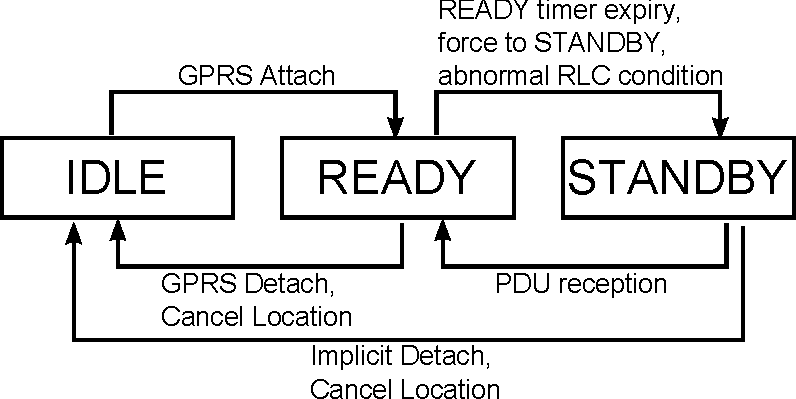
\includegraphics[width=\textwidth]{images/mm-2g-state-model.pdf}
		\caption{State machine for \acrshort{2G} radio access.}
		\label{c4:fig:2g-mmstatemodel}
	\end{subfigure}%

	\begin{subfigure}[b]{0.70\textwidth}
		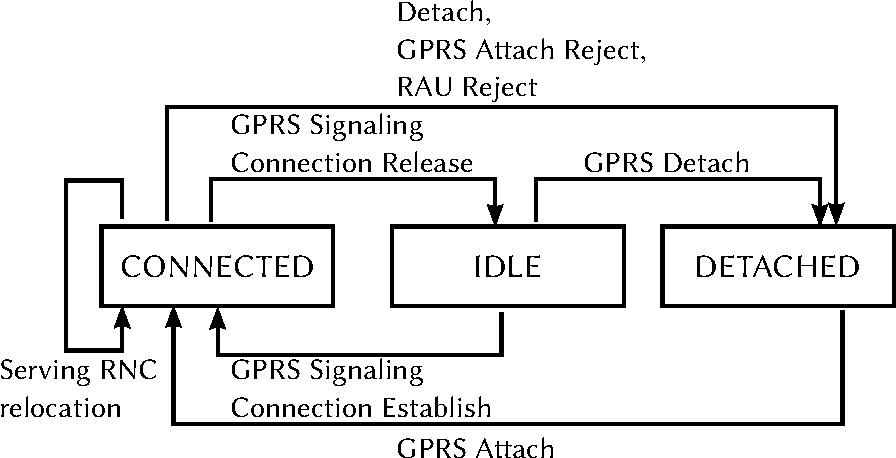
\includegraphics[width=\textwidth]{images/mm-3g-state-model.pdf}
		\caption{State machine for \acrshort{3G} radio access.}
		\label{c4:fig:3g-mmstatemodel}
	\end{subfigure}%
	\caption{\acrshort{SGSN} \acrshort{MM} state models and machines as defined in \cite[Section~6.1]{3gpp.23.060}.}
\label{c4:fig:mmstatemodel}
\end{figure}

The \gls{MM} model, defined in \cite[Section~6.1]{3gpp.23.060}, describes the general state of the data connection. State switches occur either based on an idle timer or when new packets arrive for the mobile device. The specific model depends on the currently used \gls{RAT} with only slight differences between \gls{GSM} (Figure~\ref{c4:fig:2g-mmstatemodel}) and \gls{UMTS} (Figure~\ref{c4:fig:3g-mmstatemodel}) access. The \gls{LTE} related model brings larger changes but is omitted here, as it will not be relevant for the investigation. With the transition to and from the \textbf{IDLE} state in the \gls{2G} model (or \textbf{DETACHED} in \gls{3G}) \textbf{GPRS Attach/Detach} procedures are triggered, also resulting in the transmission of \gls{PDP} Create and Delete Context messages. Likewise, other state transition procedures indicate mobility and location changes, which usually include update messages.

\begin{figure}[htb] 
	\centering
	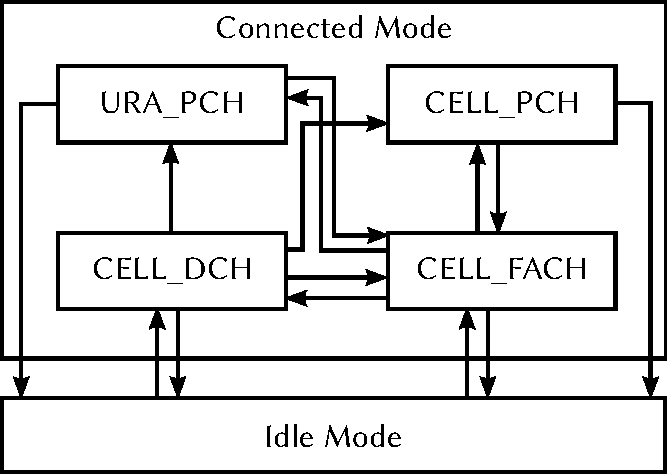
\includegraphics[width=0.4\textwidth]{images/rrc-state-model.pdf}
	\caption{\acrshort{RRC} State Model as per \cite[Section~7.1]{3gpp.25.331}.}
	\label{c4:fig:rrcstatemodel}
\end{figure}

 The \gls{RRC} state machine given in \gls{TS}~25.331~\cite[Section~7.1]{3gpp.25.331} and depicted in Figure~\ref{c4:fig:rrcstatemodel} governs the usage of radio channels and therefore power states of the \gls{MS}. State changes happen depending on user and radio activity and inactivity determined by timers. Only in the \gls{CELLDCH} state is the \gls{MS} assigned a dedicated channel for its data connection and can transmit at full bidirectionally. But this consumes the most device power and radio resources, both of which are scarce. The goal of the state machine is to minimize resource usage with intermediary states --- \gls{CELLFACH}, \gls{URAPCH}, and \gls{CELLPCH}, and  --- that successively require less power and radio channels, before completely turning of the \gls{RRC} connection by transitioning to the idle state. Coinciding with the \gls{RRC}, the \gls{CN} \gls{gtp} tunnel can also be released or needs to be reestablished. However, this is implementation specific and not precisely specified.

\begin{figure}[htb]
	\centering
	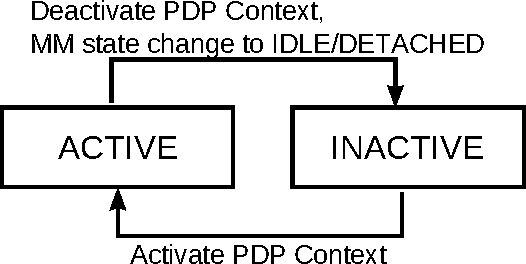
\includegraphics[width=0.35\textwidth]{images/pdp-state-model.pdf}
	\caption{\acrshort{PDP} State Model defined in \cite[Section~9]{3gpp.23.060}.}
\label{c4:fig:pdpstatemodel}
\end{figure}

The final state machine of relevancy is the \textbf{\gls{PDP} State Model} from \gls{TS}~23.060~\cite[Section~9]{3gpp.23.060} in Figure~\ref{c4:fig:pdpstatemodel}. It reflects the actual state of the \gls{PDP} context and associated tunnel and is synchronized with the \gls{MM} state machine.


%%
\subsection{Signaling Discussion}

This section on the basics of current mobile network architectures serves a critical purpose: In order to measure and evaluate network traffic one has to first understand its architecture and needs to grasp how certain traffic patterns can occur. Unfortunately, the \gls{3GPP} specifications do not make this task very easy. Typical \gls{IETF} protocols and architectures adhere to the fundamental principles of protocol layering, function separation and end-to-end. One can read a single \gls{RFC} and understand its function and directly implement it independent of the knowledge of any other specification. This is not the case in a \gls{3G} network. Functions are often spread over several protocols or nodes, necessary details essential to an implementation are spread out over several specifications without direct reference or are even completely omitted. This circumstance makes it very hard to attribute certain observed phenomena to a specific feature in the specification.

These protocols are also very heavy in terms of state and signaling inside the network. This can be the cause of unintended and hard to predict load, which will be defined and discussed in Section~\ref{c4:sec:loaddefinition}. For now, some possibly load information in relation to the Create, Update and Delete \gls{PDP} Context Request and Reply message pairs can already be deduced. Measuring the time delta between corresponding Create and Delete events obviously results in the total duration a tunnel was established. Having shorter tunnels often also means having a greater number of tunnels and therefore a higher volume of signaling messages and an increase in processing and state-keeping efforts due to the signaling. 

Conversely, longer tunnel durations cause an increased overall memory footprint in the involved nodes to store the \gls{PDP} Contexts. Large numbers of update messages, especially combined with frequent \gls{RAT} switches, are usually an indicator for highly mobile devices switching their routing area. The time between a request and its corresponding response could also be an indicator for the amount of processing involved for this message as well as the current general processing load at the \gls{GGSN}. Most of the actions in the network as well as in the mobile devices are reflected in the presented tunnel management messaging. Therefore, taking a look at the dynamics of this control aspect in real networks gives valuable insights on the influence of many of the networks' aspects.





%This section starts with a primer on cellular data network basics, and then moves on to describe relevant details of \gls{gtp}, the tunneling protocol under investigation.


% calculation: 36 element lengths + 36 * 1 Byte IE type fields + 11 byte header with no extensions
% 1012 + 36 + 11 = 1059B



% http://3gppinterview.blogspot.co.at/p/why-is-cellfach-and-cellpch-not.html <- this may be easier to understand


% \subsubsection{Information Elements Wire Format}

% \paragraph{IMSI}

% \begin{table}[htb]
% 	\caption{IMSI Information Element Format.}
% 	\label{c4:tbl:imsiieformat}
% 	\begin{tabu}{X[c]|X|X|X|X|X|X|X|X|}
% 	\multicolumn{1}{c}{} & \multicolumn{8}{c}{\textbf{Bits}} \\
% 	\cline{2-9} \textbf{Octets} & 8 & 7 & 6 & 5 & 4 & 3 & 2 & 1 \\ 
% 	\cline{2-9} 1 & \multicolumn{8}{c|}{Type = 1 (decimal)} \\ 
% 	\cline{2-9} 2 to 3 & \multicolumn{8}{c|}{Length = n}  \\ 
% 	\cline{2-9} 4 & \multicolumn{4}{c|}{Spare} & \multicolumn{4}{c|}{Instance} \\ 
% 	\cline{2-9} 5 & \multicolumn{4}{c|}{Number digit 2} & \multicolumn{4}{c|}{Number digit 1} \\ 
% 	\cline{2-9} 6 & \multicolumn{4}{c|}{Number digit 4} & \multicolumn{4}{c|}{Number digit 3} \\ 
% 	\cline{2-9} ... & \multicolumn{4}{c|}{...} & \multicolumn{4}{c|}{...} \\ 
% 	\cline{2-9} n+4 & \multicolumn{4}{c|}{Number digit m} & \multicolumn{4}{c|}{Number digit m-1} \\ 
% 	\cline{2-9}
% 	\end{tabu}
% \end{table}

% Decimals coded as TBCD; if odd number fill last nibble with 1; max digits is 15.\\
% Max IE size 12 Byte.

% \paragraph{APN}

% \begin{table}[htb]
% 	\caption{APN Information Element Format.}
% 	\label{c4:tbl:apnieformat}
% 	\begin{tabu}{X[c]|X|X|X|X|X|X|X|X|}
% 	\multicolumn{1}{c}{} & \multicolumn{8}{c}{\textbf{Bits}} \\
% 	\cline{2-9} \textbf{Octets} & 8 & 7 & 6 & 5 & 4 & 3 & 2 & 1 \\ 
% 	\cline{2-9} 1 & \multicolumn{8}{c|}{Type = 71 (decimal)} \\ 
% 	\cline{2-9} 2 to 3 & \multicolumn{8}{c|}{Length = n}  \\ 
% 	\cline{2-9} 4 & \multicolumn{4}{c|}{Spare} & \multicolumn{4}{c|}{Instance} \\ 
% 	\cline{2-9} 5 to (n+4) & \multicolumn{8}{c|}{Access Point Name} \\ 
% 	\cline{2-9}
% 	\end{tabu} 
% \end{table}

% Full APN name including APN Network Identifier and APN Operator Identifier.
% Network Identifier: max length 63 bytes.
% Operator Identifier: mnc<3digits>.mcc<3digits>.gprs; 16 bytes (18 incl dots).
% (Ex: ggsn-cluster-A.provinceB.mnc012.mcc345.gprs)

% Max total $4+63+16=83$

% \paragraph{AMBR}

% \begin{table}[htb]
% 	\caption{APN Information Element Format.}
% 	\label{c4:tbl:abmrieformat}
% 	\begin{tabu}{X[c]|X|X|X|X|X|X|X|X|}
% 	\multicolumn{1}{c}{} & \multicolumn{8}{c}{\textbf{Bits}} \\
% 	\cline{2-9} \textbf{Octets} & 8 & 7 & 6 & 5 & 4 & 3 & 2 & 1 \\ 
% 	\cline{2-9} 1 & \multicolumn{8}{c|}{Type = 72 (decimal)} \\ 
% 	\cline{2-9} 2 to 3 & \multicolumn{8}{c|}{Length = n}  \\ 
% 	\cline{2-9} 4 & \multicolumn{4}{c|}{Spare} & \multicolumn{4}{c|}{Instance} \\ 
% 	\cline{2-9} 5 to 8 & \multicolumn{8}{c|}{APN-AMBR for uplink} \\ 
% 	\cline{2-9} 9 to 12 & \multicolumn{8}{c|}{APN-AMBR for downlink} \\ 
% 	\cline{2-9}
% 	\end{tabu} 
% \end{table}

% Total size 12 bytes.


% \paragraph{Recovery}

% \begin{table}[htb]
% 	\caption{Recovery Information Element Format.}
% 	\label{c4:tbl:recoveryieformat}
% 	\begin{tabu}{X[c]|X|X|X|X|X|X|X|X|}
% 	\multicolumn{1}{c}{} & \multicolumn{8}{c}{\textbf{Bits}} \\
% 	\cline{2-9} \textbf{Octets} & 8 & 7 & 6 & 5 & 4 & 3 & 2 & 1 \\ 
% 	\cline{2-9} 1 & \multicolumn{8}{c|}{Type = 3 (decimal)} \\ 
% 	\cline{2-9} 2 to 3 & \multicolumn{8}{c|}{Length = n}  \\ 
% 	\cline{2-9} 4 & \multicolumn{4}{c|}{Spare} & \multicolumn{4}{c|}{Instance} \\ 
% 	\cline{2-9} 5 to (n+4) & \multicolumn{8}{c|}{Recovery (Restart Counter} \\ 
% 	\cline{2-9}
% 	\end{tabu} 
% \end{table}

% IN GTPv2 first release IE length is 5 bytes. May be longer in the future.


% \paragraph{MEI}

% \begin{table}[htb]
% 	\caption{MEI Information Element Format.}
% 	\label{c4:tbl:meiieformat}
% 	\begin{tabu}{X[c]|X|X|X|X|X|X|X|X|}
% 	\multicolumn{1}{c}{} & \multicolumn{8}{c}{\textbf{Bits}} \\
% 	\cline{2-9} \textbf{Octets} & 8 & 7 & 6 & 5 & 4 & 3 & 2 & 1 \\ 
% 	\cline{2-9} 1 & \multicolumn{8}{c|}{Type = 75 (decimal)} \\ 
% 	\cline{2-9} 2 to 3 & \multicolumn{8}{c|}{Length = n}  \\ 
% 	\cline{2-9} 4 & \multicolumn{4}{c|}{Spare} & \multicolumn{4}{c|}{Instance} \\ 
% 	\cline{2-9} 5 to (n+4) & \multicolumn{8}{c|}{Mobile Equipment (ME) Identity} \\ 
% 	\cline{2-9}
% 	\end{tabu}
% \end{table}

% 15 (IMEI) or 16 (IMEISV) BCD digits filled with 1 to full octet. Size is 12 bytes.

% \paragraph{MSISDN}

% \begin{table}[htb]
% 	\caption{MSISDN Information Element Format.}
% 	\label{c4:tbl:msisdnieformat}
% 	\begin{tabu}{X[c]|X|X|X|X|X|X|X|X|}
% 	\multicolumn{1}{c}{} & \multicolumn{8}{c}{\textbf{Bits}} \\
% 	\cline{2-9} \textbf{Octets} & 8 & 7 & 6 & 5 & 4 & 3 & 2 & 1 \\ 
% 	\cline{2-9} 1 & \multicolumn{8}{c|}{Type = 76 (decimal)} \\ 
% 	\cline{2-9} 2 to 3 & \multicolumn{8}{c|}{Length = n}  \\ 
% 	\cline{2-9} 4 & \multicolumn{4}{c|}{Spare} & \multicolumn{4}{c|}{Instance} \\ 
% 	\cline{2-9} 5 & \multicolumn{4}{c|}{Number digit 2} & \multicolumn{4}{c|}{Number digit 1} \\ 
% 	\cline{2-9} 6 & \multicolumn{4}{c|}{Number digit 4} & \multicolumn{4}{c|}{Number digit 3} \\ 
% 	\cline{2-9} ... & \multicolumn{4}{c|}{...} & \multicolumn{4}{c|}{...} \\ 
% 	\cline{2-9} n+4 & \multicolumn{4}{c|}{Number digit m} & \multicolumn{4}{c|}{Number digit m-1} \\ 
% 	\cline{2-9}
% 	\end{tabu}
% \end{table}

% MSISDN limited to 15 digits. Max total size 12 bytes.


% \paragraph{Indication}

% \begin{table}[htb]
% 	\caption{Indication Information Element Format.}
% 	\label{c4:tbl:indicationieformat}
% 	\begin{tabu}{X[c]|X|X|X|X|X|X|X|X|}
% 	\multicolumn{1}{c}{} & \multicolumn{8}{c}{\textbf{Bits}} \\
% 	\cline{2-9} \textbf{Octets} & 8 & 7 & 6 & 5 & 4 & 3 & 2 & 1 \\ 
% 	\cline{2-9} 1 & \multicolumn{8}{c|}{Type = 77 (decimal)} \\ 
% 	\cline{2-9} 2 to 3 & \multicolumn{8}{c|}{Length = n}  \\ 
% 	\cline{2-9} 4 & \multicolumn{4}{c|}{Spare} & \multicolumn{4}{c|}{Instance} \\ 
% 	\cline{2-9} 5 & DAF & DTF & HI & DFI & OI & ISRSI & ISRAI & SGWCI \\ 
% 	\cline{2-9} 6 & Spare & UIMSI & CFSI & CRSI & P & PT & SI & MSV \\ 
% 	\cline{2-9} 7 to (n+4) & \multicolumn{8}{c|}{These octet(s) is/are present only if explicitly specified} \\ 
% 	\cline{2-9}
% 	\end{tabu}
% \end{table}

% Size is 7 bytes.

% \paragraph{PCO}


% \begin{table}[htb]
% 	\caption{PCO Information Element Format.}
% 	\label{c4:tbl:pcoieformat}
% 	\begin{tabu}{X[c]|X|X|X|X|X|X|X|X|}
% 	\multicolumn{1}{c}{} & \multicolumn{8}{c}{\textbf{Bits}} \\
% 	\cline{2-9} \textbf{Octets} & 8 & 7 & 6 & 5 & 4 & 3 & 2 & 1 \\ 
% 	\cline{2-9} 1 & \multicolumn{8}{c|}{Type = 78 (decimal)} \\ 
% 	\cline{2-9} 2 to 3 & \multicolumn{8}{c|}{Length = n}  \\ 
% 	\cline{2-9} 4 & \multicolumn{4}{c|}{Spare} & \multicolumn{4}{c|}{Instance} \\ 
% 	\cline{2-9} 5 to (n+4) & \multicolumn{8}{c|}{Protocol Configuration Options} \\
% 	\cline{2-9}
% 	\end{tabu}
% \end{table}

% Minimum length 4+3-3, maximum length 4+253-3; average?


% \paragraph{PAA}

% \begin{table}[htb]
% 	\caption{PAA Information Element Format.}
% 	\label{c4:tbl:paaieformat}
% 	\begin{tabu}{X[c]|X|X|X|X|X|X|X|X|}
% 	\multicolumn{1}{c}{} & \multicolumn{8}{c}{\textbf{Bits}} \\
% 	\cline{2-9} \textbf{Octets} & 8 & 7 & 6 & 5 & 4 & 3 & 2 & 1 \\ 
% 	\cline{2-9} 1 & \multicolumn{8}{c|}{Type = 79 (decimal)} \\ 
% 	\cline{2-9} 2 to 3 & \multicolumn{8}{c|}{Length = n}  \\ 
% 	\cline{2-9} 4 & \multicolumn{4}{c|}{Spare} & \multicolumn{4}{c|}{Instance} \\ 
% 	\cline{2-9} 5 & \multicolumn{5}{c|}{Spare} & \multicolumn{3}{c|}{PDN Type} \\
% 	\cline{2-9} 6 to (n+4) & \multicolumn{8}{c|}{PDN Adress and Prefix} \\
% 	\cline{2-9}
% 	\end{tabu} 
% \end{table}

% Either 9 (IPv4), 22 (IPv6), or 26 (IPv4v6).


% \paragraph{RAT Type}


% \begin{table}[htb]
% 	\caption{RAT Information Element Format.}
% 	\label{c4:tbl:ratieformat}
% 	\begin{tabu}{X[c]|X|X|X|X|X|X|X|X|}
% 	\multicolumn{1}{c}{} & \multicolumn{8}{c}{\textbf{Bits}} \\
% 	\cline{2-9} \textbf{Octets} & 8 & 7 & 6 & 5 & 4 & 3 & 2 & 1 \\ 
% 	\cline{2-9} 1 & \multicolumn{8}{c|}{Type = 82 (decimal)} \\ 
% 	\cline{2-9} 2 to 3 & \multicolumn{8}{c|}{Length = n}  \\ 
% 	\cline{2-9} 4 & \multicolumn{4}{c|}{Spare} & \multicolumn{4}{c|}{Instance} \\ 
% 	\cline{2-9} 5 & \multicolumn{8}{c|}{RAT Type} \\
% 	\cline{2-9} 6 to (n+4) & \multicolumn{8}{c|}{These octet(s) is/are present only if explicitly specified} \\
% 	\cline{2-9}
% 	\end{tabu} 
% \end{table}

% Maximum length 5 to ?.

% \paragraph{Serving Network}

% \begin{table}[htb]
% 	\caption{Serving Network Information Element Format.}
% 	\label{c4:tbl:servingnetieformat}
% 	\begin{tabu}{X[c]|X|X|X|X|X|X|X|X|}
% 	\multicolumn{1}{c}{} & \multicolumn{8}{c}{\textbf{Bits}} \\
% 	\cline{2-9} \textbf{Octets} & 8 & 7 & 6 & 5 & 4 & 3 & 2 & 1 \\ 
% 	\cline{2-9} 1 & \multicolumn{8}{c|}{Type = 83 (decimal)} \\ 
% 	\cline{2-9} 2 to 3 & \multicolumn{8}{c|}{Length = n}  \\ 
% 	\cline{2-9} 4 & \multicolumn{4}{c|}{Spare} & \multicolumn{4}{c|}{Instance} \\ 
% 	\cline{2-9} 5 & \multicolumn{4}{c|}{MCC digit 2} & \multicolumn{4}{c|}{MCC digit 1} \\ 
% 	\cline{2-9} 6 & \multicolumn{4}{c|}{MNC digit 3} & \multicolumn{4}{c|}{MCC digit 3} \\ 
% 	\cline{2-9} 7 & \multicolumn{4}{c|}{MNC digit 2} & \multicolumn{4}{c|}{MNC digit 1} \\ 
% 	\cline{2-9} 8 to (n+4) & \multicolumn{8}{c|}{These octet(s) is/are present only if explicitly specified} \\
% 	\cline{2-9}
% 	\end{tabu}
% \end{table} 

% Maximum length 7 to ?.


% \paragraph{User Location Information}

% \begin{table}[htb]
% 	\caption{User Location Information Element Format.}
% 	\label{c4:tbl:userlocieformat}
% 	\begin{tabu}{X[c]|X|X|X|X|X|X|X|X|}
% 	\multicolumn{1}{c}{} & \multicolumn{8}{c}{\textbf{Bits}} \\
% 	\cline{2-9} \textbf{Octets} & 8 & 7 & 6 & 5 & 4 & 3 & 2 & 1 \\ 
% 	\cline{2-9} 1 & \multicolumn{8}{c|}{Type = 86 (decimal)} \\ 
% 	\cline{2-9} 2 to 3 & \multicolumn{8}{c|}{Length = n}  \\ 
% 	\cline{2-9} 4 & \multicolumn{4}{c|}{Spare} & \multicolumn{4}{c|}{Instance} \\ 
% 	\cline{2-9} 5 & \multicolumn{3}{c|}{Spare} & ECGI & TAI & RAI & SAI & CGI \\ 
% 	\cline{2-9} a to a+6 & \multicolumn{8}{c|}{CGI} \\ 
% 	\cline{2-9} 7 & \multicolumn{8}{c|}{SAI} \\ 
% 	\cline{2-9} 7 & \multicolumn{8}{c|}{RAI} \\ 
% 	\cline{2-9} 7 & \multicolumn{8}{c|}{TAI} \\ 
% 	\cline{2-9} 7 & \multicolumn{8}{c|}{ECGI} \\ 
% 	\cline{2-9} 8 to (n+4) & \multicolumn{8}{c|}{These octet(s) is/are present only if explicitly specified} \\
% 	\cline{2-9}
% 	\end{tabu} 
% \end{table}



% Information Elements Table for PDP Context Activation Case only for GTPv2 (LTE)
% \begin{longtabu} to\linewidth{| X[2,l] | X[2,c] | X[l] | X[4] |}
% \hline
% Information Element 						& IE Type 					& Max Wire Size (Bytes)	& Comment \\ \hline
% \gls{IMSI} 										& IMSI 						& 12					& \\ \hline
% \gls{MSISDN} 										& MSISDN					& 12					& On S11 Interface if provided by HSS; In case of UE requested connectivity if MME has it stored. \\ \hline
% MEI Identity 								& MEI 						& 12					& If available at MME. \\ \hline
% User Location Information 					& ULI						& 						& E-UTRAN initial attach \&  UE requested connectivity only; included by S-GW if received from MME via S5/S8; included on S4 and S5/S8 for PDP context activation, either CGI, SAI, or RAI. \\ \hline
% Serving Network								& Serving Network			& 						& Initial E-UTRAN attach, context activation and UE requested connectivity \\ \hline
% \gls{RAT} Type									& RAT Type					& 5						& \\ \hline
% Indication Flags							& Indication				& 6						& Flags: S5/S8 Protocol Type; Dual Address Bearer Flag; Handover Indication; Direct Tunnel Flag; Piggybacking Supported; Change Reporting Support Indication \\ \hline
% Sender F-TEID for Control Plane				& F-TEID					& 						& \\ \hline
% P-G S5/S8 Address for Control Plane or PMIP	& F-TEID					& 						& On S11/S4 interfaces; 0 if initial attach, context activation or PDN connectivity \\ \hline
% Access Point Name							& APN						& 83					& \\ \hline
% Selection Mode								& Selection Mode			& 						& Indicate whether subscribed or non-subscribed, chosen by MME, was selected \\ \hline
% PDN Type									& PDN Type					& 						& IPv4, IPv6 or IPv4v6. \\ \hline
% PDN Address Allocation						& PAA						& 26					& Set to static IP address; else (dynamic) to 0.0.0.0 or IPv6 Prefix Length 0. \\ \hline
% Maximum APN Restriction						& APN Restriction			& 						& Set to most stringent restriction of any active bearer. \\ \hline
% Aggregate Maximum Bit Rate					& ABMR						& 12					& \\ \hline
% Protocol Configuration Options				& PCO						& 254					& Forwarded from UE to P-GW via S-GW via MME. \\ \hline
% Bearer Contexts to be created				& Bearer Context			& 						& present multiple times to represent list of bearers \\ \hline
% Trace Information							& Trace Information 		& 						& If S-GW / P-GW is activated. \\ \hline
% Recovery									& Recovery					& 5						& If peer node contacted for the first time. \\ \hline
% MME-FQ-CSID									& FQ-CSID					& 						& Included by MME on S11 \\ \hline
% SGW-FQ-CSID									& FQ-CSID					& 						& Included by SGW on S5/S8 \\ \hline
% UE Time Zone								& UE Time Zone 				& 						& Can be included by MME on S11; forwarded to P-GW via S-GW \\ \hline
% User CSG Information						& UCI						& 						& If \gls{UE} accessed via CSG cell or hybrid cell \\ \hline
% Charging Characteristics					& Charging Characteristics	&						& \\ \hline
% Private Extensions							& Private Extensions		&						& \\ \hline
% \end{longtabu}





% \begin{figure}[htb]
% 	\centering
%  	\includegraphics[width=0.9\textwidth]{images/eNB-MME-layers.pdf}
%  	\caption{Control plane protocol stack at the S1-MME interface between eNodeB and MME.}
%  	\label{c4:fig:stack-enbmme}
% \end{figure}

% \begin{figure}[htb]
% 	 \centering
% 	 \includegraphics[width=0.9\textwidth]{images/SGSN-MME-layers.pdf}
% 	 \caption{Control plane protocol stack at the S3 interface between SGSN and MME.}
% 	 \label{c4:fig:stack-sgsnmme}
% \end{figure}

% \begin{figure}[htb]
% 	\centering
% 	\includegraphics[width=0.9\textwidth]{images/S-GW-P-GW-layers.pdf}
% 	\caption{Optional control plane protocol stack at the S5 interface between SGW and PGW.}
% 	\label{c4:fig:stack-sgwpgw}
% \end{figure}

% \begin{figure}[htb]
% 	\centering
% 	\includegraphics[width=0.9\textwidth]{images/MME-S-GW-layers.pdf}
% 	\caption{Control plane protocol stack at the S11 interface between MME and SGW.}
% 	\label{c4:fig:stack-mmesgw}
% \end{figure}



%List of interfaces in the 3G/LTE PS network
%\begin{itemize}
%\item \textbf{Uu}: Interface between the mobile station (MS) and the fixed network part in Iu mode. The Uu interface is the Iu mode network interface for providing packet data services over the radio to the MS. The MT part of the MS is used to access the UMTS services through this interface.
%\item \textbf{Iub}: Interface between a NodeB and a RNC.
%\item \textbf{IuPS}: Interface between a RNC and a SGSN.
%\item \textbf{S1-U}: Interface between a eNodeB and a S-GW. User plane bearer tunneling.
% \item \textbf{S1-MME}: Interface between a eNodeB and a MME.
% \item \textbf{S3}: Interface between a SGSN and a MME. User/bearer information exchange for active/idle state 3g network access mobility.
% \item \textbf{S4}: Interface between a SGSN and a S-GW.	 2G user plane tunneling. GPRS mobility and control.
% \item \textbf{S5}: Interface between a S-GW and a P-GW within the same PLMN. User plane tunneling; S-GW relocation due to mobility.
% \item \textbf{S6a}: Interface between a MME and a HSS. Auth/auth data transfer to evolved system.
% \item \textbf{Gr/S6d}: Interface between a SGSN and a HSS. 
% \item \textbf{S8}: Interface between a S-GW and a P-GW in different PLMNs. Inter-PLMN variant to S5.
% \item \textbf{S9}: Interface between a PRCF and the packet data network. Data exchange to visited PCRF PLMN.
% \item \textbf{S11}: Interface between a S-GW and a MME.
% \item \textbf{S12}: UTRAN to S-GW reference point. Based on Iu-u/Gn-u. Direct Tunnel via GTP-U.
% \item \textbf{S13}: Interface between a MME and a EIR. UE identity check.
% \item \textbf{SGi}: The reference point between the EPC based PLMN and the packet data network. Same as Gi for 3gpp.

% \item \textbf{GC}: Interface between a HSS and a GGSN.
% \item \textbf{Gf}: Interface between a SGSN and a EIR.
% \item \textbf{Gi}: Reference point between Packet Domain and an external packet data network.
% \item \textbf{Gn}: Interface between two GSNs within the same PLMN.
% \item \textbf{Gp}: Interface between two GSNs in different PLMNs. The Gp interface allows support of Packet Domain network services across areas served by the co-operating PLMNs.
% \item \textbf{Gx}: Interface between a PCRF and a P-GW/GGSN. QoS policy and charging rules transfer.
% \item \textbf{Gxc}: Interface between a PCRF and a S-GW.

% \item \textbf{Rx}: Interface between a PRCF and the packet data network.
% \end{itemize}


%EMM Service request procedure
% \begin{figure}[htb]
% 	\centering
% 	\includegraphics[width=1.0\textwidth]{images/UE-service-request.pdf}
% 	\caption{EMM service request procedure sequence diagram.}
% 	\label{c4:fig:3gpp-ueservicereq}
% \end{figure}

% Annotations:
% 1. Encapsulated in RRC message.
% 2. Forwarded in S1-AP Initial UE Message.
% 3. Various security procedures.

%	25.401 \cite{3gpp.25.401} UTRAN overall description
%	25.931 \cite{3gpp.25.931} UTRAN functions, examples on signalling procedures
%	23.401 \cite{3gpp.23.401} \gls{E-UTRAN} procedures (LTE only)
%	24.007 \cite{3gpp.24.007} radio interface signaling % only Um interface in plain GSM/GPRS
%	36.300 \cite{3gpp.36.300} \gls{E-UTRAN} description (LTE only) 
%	36.414 \cite{3gpp.36.414} Evolved Universal Terrestrial Radio Access Network (E-UTRAN); S1 data transport (radio bearer)
%	22.060 \cite{3gpp.22.060} basic and short \gls{GPRS} service description; unchanged since Release 6 (2004)
%	23.060 \cite{3gpp.23.060} \gls{GPRS} description : \gls{GPRS} specific procedures, interfaces and nodes; mobility management; radio management; packet routing; operational aspects



	%23.402 \cite{3gpp.23.402} (LTE only) non-\gls{3GPP} accesses
	%24.301 \cite{3gpp.24.301} EPS Non-Access-Stratum protocol between UE and MME on Uu

% Relevant protocols and interfaces between nodes:
% \begin{itemize}
% 	\item \gls{gtp}, \gls{gtpv2}, GTP-u, GTP-c, \gls{SGSN} to \gls{GGSN} and others (specify!), on top of \gls{UDP}, GTPv1 will be described in detail in a separate section as it is at the core of the upcoming investigations.
% 	\item \gls{MAP} / \gls{SS7}: \gls{SGSN} - \gls{HLR}, \gls{GGSN} - \gls{HLR} and others; subscriber management and information exchange
% 	\item Diameter \cite{rfc6733}: \gls{MME} - \gls{HSS}, \gls{SGSN} - \gls{HSS}, replacement for \gls{MAP}, subscriber management

% 	\item PMIPv6 on \gls{SGW} - \gls{PGW}, alternative tunneling protocol to GTPv2
% \end{itemize}


% \begin{figure}[htb]
% 	\centering
% 	\includegraphics[width=1.0\textwidth]{images/3g-userplane.pdf}
% 	\caption{User plane protocol stack in an UMTS network.}
% 	\label{c4:fig:3gpp-umtsuserplane}
% \end{figure}

% \begin{figure}[htb]
% 	\centering
% 	\includegraphics[width=1.2\textwidth]{images/LTE-userplane.pdf}
% 	\caption{User plane protocol stack in an LTE/EPC network.}
% 	\label{c4:fig:3gpp-lteuserplane}
% \end{figure}

% \begin{figure}[htb]
% 	\centering
% 	\includegraphics[width=1.0\textwidth]{images/bearers.pdf}
% 	\caption{3GPP bearer model.}
% 	\label{c4:fig:3gpp-bearers}
% \end{figure}


% \begin{figure}[htb]
% 	\centering
% 	\includegraphics[width=1.2\textwidth]{images/ECM-states.pdf}
% 	\caption{\gls{ECM} state machine.}
% 	\label{c4:fig:3gpp-ecmstates}
% \end{figure}


% \begin{figure}[htb]
% 	\centering
% 	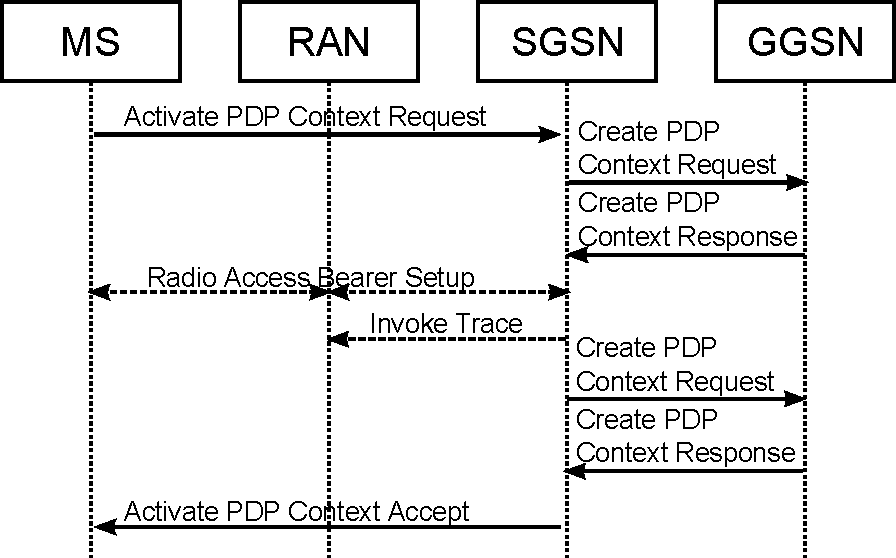
\includegraphics[width=0.8\columnwidth]{images/pdp-context-activation.pdf}
% 	\caption{PDP Context Activation Procedure in a UMTS network.}
% 	\label{c4:fig:pdpcontextactivation}
% \end{figure}



% \begin{itemize}
% \item 	Every bearer has a predefined QoS level between UE and P-GW.
% 		==> Level of Granularity for QoS control.
% \item	Initial bearer QoS level assigned by network based on subscription data.
% \item	Guaranteed Bit Rate (GBR) bearers: dedicated network resources permanently allocated at est/mod. Otherwise Non-GBR.
% \item	The Traffic Flow Template (TFT) belonging to a bearer is a set of packet filters that assign traffic flows to the bearer.
% \item	UL-TFT at UE, DL-TFT at \gls{PCEF} (P-GW).
% \item 	default bearer: always-on IP connectivity for the UE to a PDN
% \item	dedicated bearer:   
% 			\begin{itemize}
% 				\item any additional bearer for the same PDN
% 				\item \gls{TFT} associated with every ded. bearer
% 				\item establishment/modification decision only by \gls{EPC}
% 				\item QoS level assignment only by \gls{EPC}
% 			\end{itemize}

% \item	default bearer may be used as {m,c}atch-all traffic bearer for everything that does not match any filter
% \item	Every bearer associated with QCI and ARP.

% QoS class identifier (QCI): standardized scalar as reference for node-specific QoS parameters
% Allocation and Retention Policy (ARP): priority level preemption capability, preemption vulnerability.

% \item	All simultaneously active bearers by one UE are provided are provided by the same P-GW.
% \end{itemize}

% \begin{figure}[htb]
% 	\centering
% 	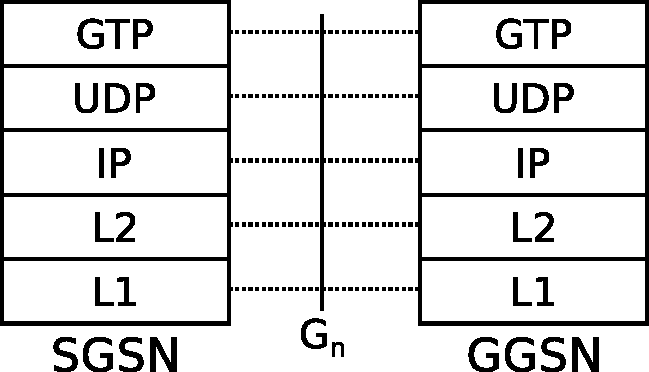
\includegraphics[width=0.6\columnwidth]{images/signalling-stack.pdf}
% 	\caption{Typical signaling protocol stack at the Gn interface between \gls{SGSN} and \gls{GGSN}.}
% 	\label{c4:fig:signallingstack}
% \end{figure}

% \begin{table}[htb]
% 	\caption{GTP header format (TODO: which one exactly. This looks like v2-U but should actually better be v1!)}
% 	\label{c4:tbl:gtpheader}
% 	\begin{tabu}{c|c|c|c|c|c|c|c|c|}
% 	\multicolumn{1}{c}{} & \multicolumn{8}{c}{\textbf{Bits}} \\
% 	\cline{2-9} \textbf{Octets} & 8 & 7 & 6 & 5 & 4 & 3 & 2 & 1 \\ 
% 	\cline{2-9} 1 & \multicolumn{3}{c|}{Version}  & P & T & Spare & Spare & Spare \\ 
% 	\cline{2-9} 2 & \multicolumn{8}{c|}{Message Type}  \\ 
% 	\cline{2-9} 3 & \multicolumn{8}{c|}{Message Length (1st Octet)}  \\ 
% 	\cline{2-9} 4 & \multicolumn{8}{c|}{Message Length (2nd Octet)}  \\ 
% 	\cline{2-9} m to & \multicolumn{8}{c|}{\multirow{2}{10cm}{If T flag is set to 1, then TEID shall be placed into octets 5-8. Otherwise, TEID field is not present at all.}} \\ 
% 	 k(m+3) & \multicolumn{8}{c|}{} \\ 
% 	\cline{2-9} n to (n+2) & \multicolumn{8}{c|}{Sequence Number} \\ 
% 	\cline{2-9} (n+3) & \multicolumn{8}{c|}{Spare} \\ 
% 	\cline{2-9} 
% 	\end{tabu} 
% \end{table}


%LTE: mention also \gls{PMIPv6} as \gls{gtp} alternative, and the option to have a combined \gls{SGW} \gls{PGW}


% request/response messaging
% response types:
% Possible context response types and which request types they answer:
% \begin{itemize}
% \item 192: ``non-existent'' UPDATE \& DELETE ONLY
% \item 193: ``invalid message format'' UPDATE \& DELETE ONLY
% \item 199: ``no resources available'' CREATE ONLY anywhere in the network to allocate context
% \item 200: ``service not supported'' UPDATE ONLY
% \item 201: ``mandatory IE incorrect''
% \item 202: ``mandatory IE missing''
% \item 204: ``system failure'' CREATE \& UPDATE ONLY
% \item 209: ``user authentication failed'' CREATE ONLY rejected for various reasons
% \end{itemize}

%---
%NSAPI {0;15} Integer
%linked \gls{NSAPI}: indicates the \gls{NSAPI} assigned to any one of the already activated \gls{PDP} contexts for this address/phone ("foreign key"?)

% TODO: convert to UMTS

% \begin{figure}[htb]
% 	\centering
% 	\includegraphics[width=1.0\textwidth]{images/UE-requested-PDN-connectivity.pdf}
% mdcm	\caption{\gls{PDN} connectivity request by the UE procedure sequence diagram.}
% 	\label{c4:fig:3gpp-uepdnreq}
% \end{figure}


%% creates
%IPv6 Stateless Address Autoconfiguration Procedure
%PDP Context Activation Procedure for A/Gb mode (additional (optional?) update pair)
%PDP Context Activation Procedure for Iu mode (additional (optional?) update pair)
%Secondary PDP Context Activation for Iu mode (additional (optional?) update pair)
%Secondary PDP Context Activation for A/Gb mode (additional (optional?) update pair)

%% deletes
%MS Initiated PDP Context Deactivation Procedure for A/Gb mode
%MS Initiated PDP Context Deactivation Procedure for Iu mode
%SGSN-initiated PDP Context Deactivation Procedure
%GGSN-initiated PDP Context Deactivation Procedure
%Combined GPRS/IMSI Attach Procedure (2x request+response, 1 to old, 1 to new)
%MS-Initiated Detach Procedure (1x request/response)
%Network-Initiated Detach Procedures (SGSN or HLR)


%% updates
%Inter SGSN Routeing Area Update (1x)
%Combined Inter SGSN RA/LA Update (1x)
%Iu mode RA Update Procedure (1x)
%SRNS Serving Radio Network Subsystem Relocation Procedure (1x)
%Combined Hard Handover and SRNS Relocation Procedure
%Combined Cell/URA (UTRAN Registration Area) Update and SRNS Relocation Procedure
%Enhanced Serving RNS Relocation
%Iu mode to A/Gb mode Intra SGSN Change
%Iu mode to A/Gb mode Inter SGSN Change
%A/Gb mode to Iu mode Inter SGSN Change
%SGSN-Initiated PDP Context Modification Procedure, A/Gb mode (2x pair (1 optional?))
%SGSN-Initiated PDP Context Modification Procedure, Iu mode (2x pair (1 optional?))
%GGSN-Initiated PDP Context Modification Procedure, Iu mode
%GGSN-Initiated PDP Context Modification Procedure, A/Gb mode
%MS-Initiated PDP Context Modification Procedure, A/Gb mode (2x, 1 optional/conditional)
%MS-Initiated PDP Context Modification Procedure, Iu mode (2x, 1 optional/conditional)
%PDP Context Activation Procedure for A/Gb mode (additional (optional?) update pair)
%PDP Context Activation Procedure for Iu mode (additional (optional?) update pair)
%Secondary PDP Context Activation for Iu mode (additional (optional?) update pair)
%Secondary PDP Context Activation for A/Gb mode (additional (optional?) update pair)
%RAB Release Procedure Using Gn/Gp (conditional if direct tunnel and context to be preserved)
%Iu Release Procedure Using Gn/Gp (conditional if direct tunnel and context to be preserved)
%RAB Assignment Procedure Using Gn/Gp (conditional direct tunnel)

%%%%%%%%%%%%%%%%%%%%%%%%%%%%%%%%%%%%%%%%%%%%%%%%%%%%%%%%%%%%%%%%%%%%%%%%%%%%%%%%
%%!TEX root = dissertation.tex
%%%%%%%%%%%%%%%%%%%%%%%%%%%%%%%%%%%%%%%%%%%%%%%%%%%%%%%%%%%%%%%%%%%%%%%%%%%%%%%%
%
% Collection of all relevant mobile radio specifications and descriptions
%
\section{Übersicht}

\begin{itemize}
\item Einarbeitung
	\begin{itemize}
		\item Architektur von 3G-Netzen
		\item Modelle zur Beschreibung von Datenverkehrsflüssen
		\item Einarbeitung in das Messsystem des FTW
	\end{itemize}
\item Definition eines einfachen Bearer-Modells
\item Programmierung der Auswertung
\item Durchführung und Auswertung der Messungen
\item Anfertigung eines Berichtes
\end{itemize}

\section{Modeling}
Macroscopic Behavior

	-- time Connection Setup until Call Termination with Talk Spurts
	--> ON/OFF Process
	--> Empricial measurement
	
Source Traffic Model
	-- 2 parts: 
		arrival process for user activities
		process describing activity phase
	-- arrival time:
		User begins web browsing
	
Simulation \& Software
	ns-2 UMTS mobile parts only
	ns-3 GSoC2010 implementing \ac{UTRAN} (MAC\&PHY) incl radio bearers (+OpenFlow)
	Harald Welte GPRS: OpenBSC, OpenGGSN incl GTP
	

EPS first introduced in 3GPP Release 8, completed in March 2009. Consisting of EUTRAN, EPC (formerly SAE)


	


\begin{figure}[htbp]
 \centering
 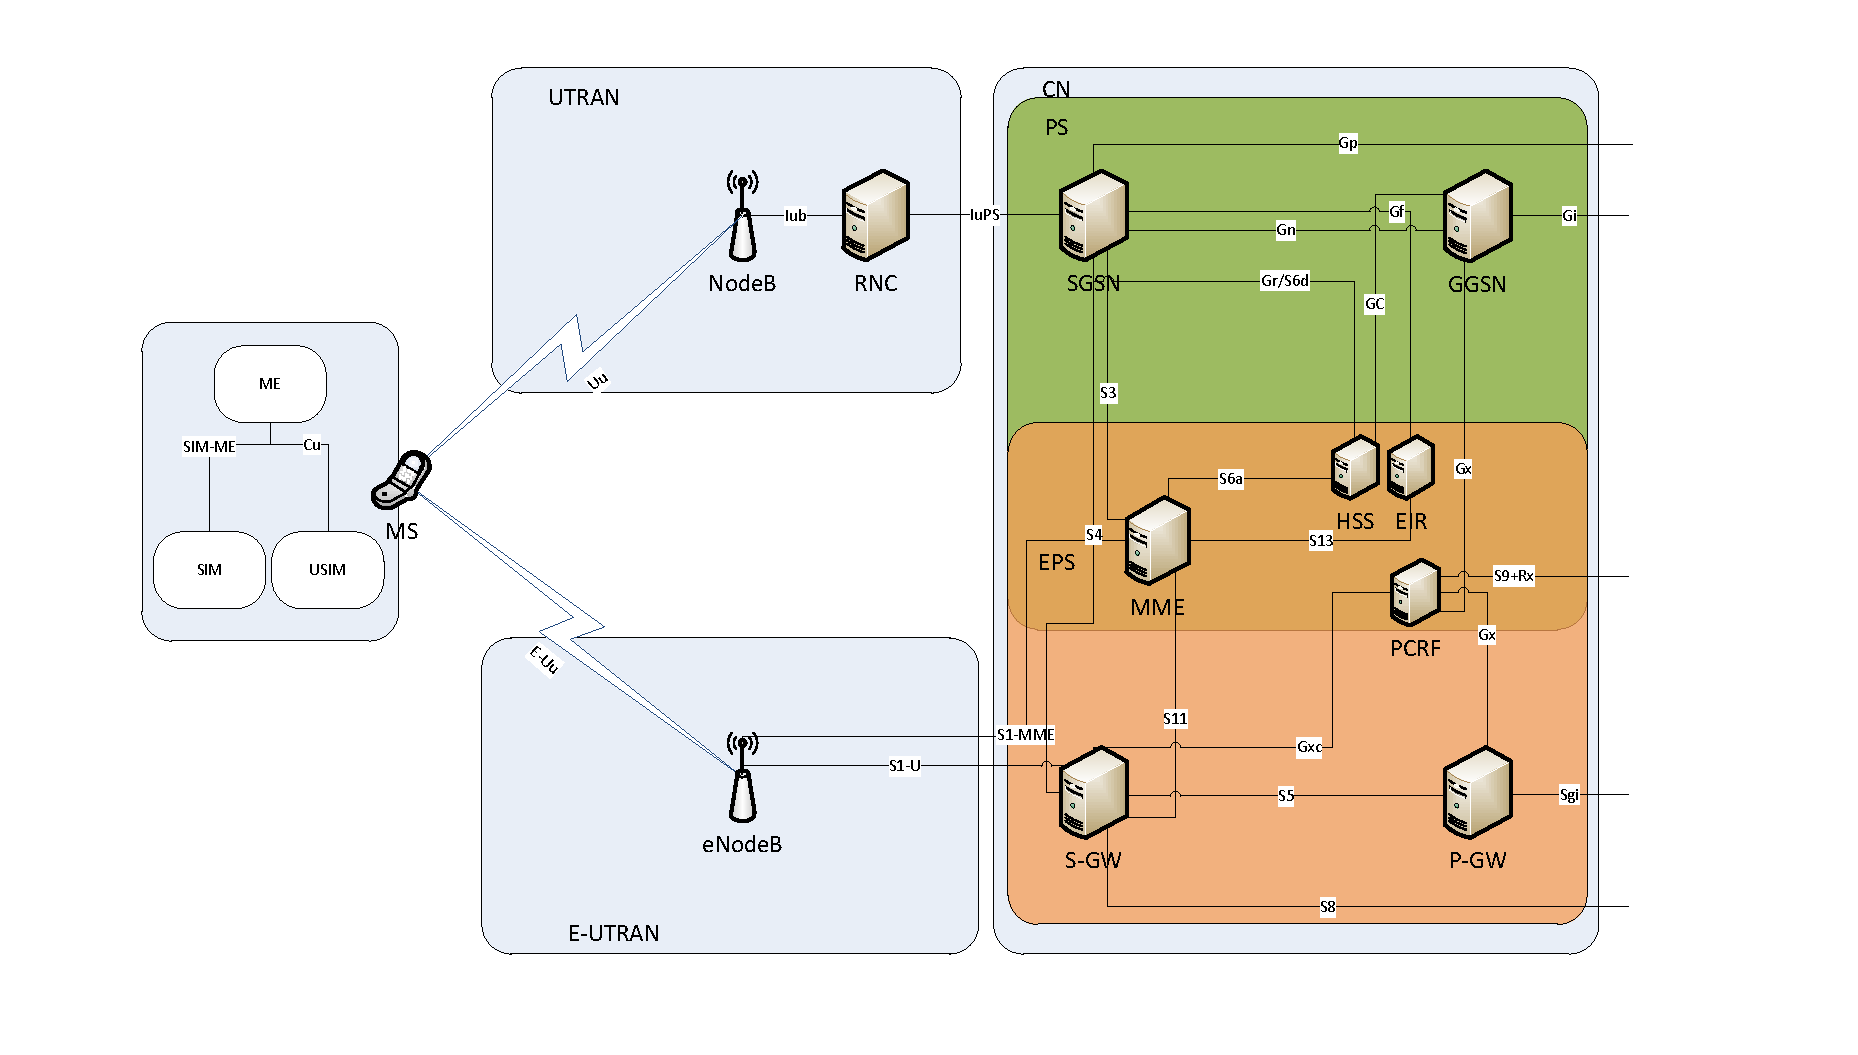
\includegraphics[width=1.0\textwidth]{images/3gpp/eps_ps-overview.pdf}
 \caption{Beispielnetz}\label{fig:netzwerk2}
\end{figure}

List of interfaces in the 3G/LTE PS network
\begin{itemize}
\item \textbf{Uu}: Interface between the mobile station (MS) and the fixed network part in Iu mode. The Uu interface is the Iu mode network interface for providing packet data services over the radio to the MS. The MT part of the MS is used to access the UMTS services through this interface.
\item \textbf{Iub}: Interface between a NodeB and a RNC.
\item \textbf{IuPS}: Interface between a RNC and a SGSN.

\item \textbf{S1-U}: Interface between a eNodeB and a S-GW. User plane bearer tunneling.
\item \textbf{S1-MME}: Interface between a eNodeB and a MME.
\item \textbf{S3}: Interface between a SGSN and a MME. User/bearer information exchange for active/idle state 3g network access mobility.
\item \textbf{S4}: Interface between a SGSN and a S-GW.	 2G user plane tunneling. GPRS mobility and control.
\item \textbf{S5}: Interface between a S-GW and a P-GW within the same PLMN. User plane tunneling; S-GW relocation due to mobility.
\item \textbf{S6a}: Interface between a MME and a HSS. Auth/auth data transfer to evolved system.
\item \textbf{Gr/S6d}: Interface between a SGSN and a HSS. 
\item \textbf{S8}: Interface between a S-GW and a P-GW in different PLMNs. Inter-PLMN variant to S5.
\item \textbf{S9}: Interface between a PRCF and the packet data network. Data exchange to visited PCRF PLMN.
\item \textbf{S11}: Interface between a S-GW and a MME.
\item \textbf{S12}: UTRAN to S-GW reference point. Based on Iu-u/Gn-u. Direct Tunnel via GTP-U.
\item \textbf{S13}: Interface between a MME and a EIR. UE identity check.
\item \textbf{SGi}: The reference point between the EPC based PLMN and the packet data network. Same as Gi for 3gpp.

\item \textbf{GC}: Interface between a HSS and a GGSN.
\item \textbf{Gf}: Interface between a SGSN and a EIR.
\item \textbf{Gi}: Reference point between Packet Domain and an external packet data network.
\item \textbf{Gn}: Interface between two GSNs within the same PLMN.
\item \textbf{Gp}: Interface between two GSNs in different PLMNs. The Gp interface allows support of Packet Domain network services across areas served by the co-operating PLMNs.
\item \textbf{Gx}: Interface between a PCRF and a P-GW/GGSN. QoS policy and charging rules transfer.
\item \textbf{Gxc}: Interface between a PCRF and a S-GW.

\item \textbf{Rx}: Interface between a PRCF and the packet data network.
\end{itemize}

\section{Control Plane Protocol Stacks}

\begin{figure}[htbp]
 \centering
 \includegraphics[width=1.0\textwidth]{images/3gpp/eNB-MME-layers.pdf}
 \caption{Beispielnetz}\label{fig:3gpp-enbmme}
\end{figure}

\begin{figure}[htbp]
 \centering
 \includegraphics[width=1.0\textwidth]{images/3gpp/SGSN-MME-layers.pdf}
 \caption{Beispielnetz}\label{fig:3gpp-sgsnmme}
\end{figure}

\begin{figure}[htbp]
 \centering
 \includegraphics[width=1.0\textwidth]{images/3gpp/S-GW-P-GW-layers.pdf}
 \caption{Beispielnetz}\label{fig:3gpp-sgwpgw}
\end{figure}

\begin{figure}[htbp]
 \centering
 \includegraphics[width=1.0\textwidth]{images/3gpp/MME-S-GW-layers.pdf}
 \caption{Beispielnetz}\label{fig:3gpp-mmesgw}
\end{figure}


\begin{figure}[htbp]
 \centering
 \includegraphics[width=1.0\textwidth]{images/3gpp/3g-userplane.pdf}
 \caption{Beispielnetz}\label{fig:3gpp-umtsuserplane}
\end{figure}

\begin{figure}[htbp]
 \centering
 \includegraphics[width=1.0\textwidth]{images/3gpp/LTE-userplane.pdf}
 \caption{Beispielnetz}\label{fig:3gpp-lteuserplane}
\end{figure}


\section{Bearers}

As you said only 11 bearer are permitted.
So PDN connection(Default bearer) + Dedicated bearers put together should not exceed 11 bearers at any instant of time at UE side.
Theoretically 11 PDN connections are possible. But i dont think it will be of any use in practical EPS topology.

One UE Can have Maximum 3 PDN connection.
where as my knowledge is concern one UE can support maximum 11 bearers, 3 default and 8 dedicated bearers.

Does I will get in any spec for this. As the default bearer are of  NON-GBR type and and there are 5-9 are of NON-GBR QCI so I think a ue can have maximum 5 default bearer If two default bearer can not use same QCI.

\begin{figure}[htbp]
 \centering
 \includegraphics[width=1.0\textwidth]{images/3gpp/bearers.pdf}
 \caption{Beispielnetz}\label{fig:3gpp-bearers}
\end{figure}


\begin{figure}[htbp]
 \centering
 \includegraphics[width=1.0\textwidth]{images/3gpp/ECM-states.pdf}
 \caption{Beispielnetz}\label{fig:3gpp-ecmstates}
\end{figure}

\begin{itemize}
\item 	Every bearer has a predefined QoS level between UE and P-GW.
		==> Level of Granularity for QoS control.
\item	Initial bearer QoS level assigned by network based on subscription data.
\item	Guaranteed Bit Rate (GBR) bearers: dedicated network resources permanently allocated at est/mod. Otherwise Non-GBR.
\item	The Traffic Flow Template (TFT) belonging to a bearer is a set of packet filters that assign traffic flows to the bearer.
\item	UL-TFT at UE, DL-TFT at PCEF (P-GW).
\item 	default bearer: always-on IP connectivity for the UE to a PDN
\item	dedicated bearer:   
			\begin{itemize}
				\item any additional bearer for the same PDN
				\item Traffic Flow Template (TFT) associated with every ded. bearer
				\item establishment/modification decision only by EPC
				\item QoS level assignment only by EPC
			\end{itemize}

\item	default bearer may be used as {m,c}atch-all traffic bearer for everything that does not match any filter
\item	Every bearer associated with QCI and ARP.

QoS class identifier (QCI): standardized scalar as reference for node-specific QoS parameters
Allocation and Retention Policy (ARP): priority level preemption capability, preemption vulnerability.

\item	All simultaneously active bearers by one UE are provided are provided by the same P-GW.
\end{itemize}

EMM Service request procedure

\begin{figure}[htbp]
 \centering
 \includegraphics[width=1.0\textwidth]{images/3gpp/UE-service-request.pdf}
 \caption{Beispielnetz}\label{fig:3gpp-ueservicereq}
\end{figure}

Annotations:
1. Encapsulated in RRC message.
2. Forwarded in S1-AP Initial UE Message.
3. Various security procedures.


\section{Information Storage}
per PLMN node, cf. 3GPP TS 23.401 clause 5.7.

\begin{figure}[htbp]
 \centering
 \includegraphics[width=1.0\textwidth]{images/3gpp/UE-requested-PDN-connectivity.pdf}
 \caption{Beispielnetz}\label{fig:3gpp-uepdnreq}
\end{figure}


\section{GTP}
\subsection{GTPv2}



\begin{tabular}{c|c|c|c|c|c|c|c|c|}
\multicolumn{1}{c}{} & \multicolumn{8}{c}{\textbf{Bits}} \\
\cline{2-9} \textbf{Octets} & 8 & 7 & 6 & 5 & 4 & 3 & 2 & 1 \\ 
\cline{2-9} 1 & \multicolumn{3}{c|}{Version}  & P & T & Spare & Spare & Spare \\ 
\cline{2-9} 2 & \multicolumn{8}{c|}{Message Type}  \\ 
\cline{2-9} 3 & \multicolumn{8}{c|}{Message Length (1st Octet)}  \\ 
\cline{2-9} 4 & \multicolumn{8}{c|}{Message Length (2nd Octet)}  \\ 
\cline{2-9} m to & \multicolumn{8}{c|}{\multirow{2}{10cm}{If T flag is set to 1, then TEID shall be placed into octets 5-8. Otherwise, TEID field is not present at all.}} \\ 
 k(m+3) & \multicolumn{8}{c|}{} \\ 
\cline{2-9} n to (n+2) & \multicolumn{8}{c|}{Sequence Number} \\ 
\cline{2-9} (n+3) & \multicolumn{8}{c|}{Spare} \\ 
\cline{2-9} 
\end{tabular} 
\subsection{GTP-C}

\begin{tabular}{c|c|c|c|c|c|c|c|c|}
\multicolumn{1}{c}{} & \multicolumn{8}{c}{\textbf{Bits}} \\
\cline{2-9} \textbf{Octets} & 8 & 7 & 6 & 5 & 4 & 3 & 2 & 1 \\ 
\cline{2-9} 1 & \multicolumn{3}{c|}{Version}  & P & T=1 & Spare & Spare & Spare \\ 
\cline{2-9} 2 & \multicolumn{8}{c|}{Message Type}  \\ 
\cline{2-9} 3 & \multicolumn{8}{c|}{Message Length (1st Octet)}  \\ 
\cline{2-9} 4 & \multicolumn{8}{c|}{Message Length (2nd Octet)}  \\ 
\cline{2-9} 5 & \multicolumn{8}{c|}{Tunnel Endpoint Identifier (1st Octet)} \\ 
\cline{2-9} 6 & \multicolumn{8}{c|}{Tunnel Endpoint Identifier (2nd Octet)} \\ 
\cline{2-9} 7 & \multicolumn{8}{c|}{Tunnel Endpoint Identifier (3rd Octet)} \\ 
\cline{2-9} 8 & \multicolumn{8}{c|}{Tunnel Endpoint Identifier (4th Octet)} \\ 
\cline{2-9} 9 & \multicolumn{8}{c|}{Sequence Number (1st Octet)} \\
\cline{2-9} 10 & \multicolumn{8}{c|}{Sequence Number (2nd Octet)} \\
\cline{2-9} 11 & \multicolumn{8}{c|}{Sequence Number (3rd Octet)} \\
\cline{2-9} 12 & \multicolumn{8}{c|}{Spare} \\
\cline{2-9}
\end{tabular} 

12 Byte GTPv2-C header.

\subsubsection{Create Session Request Message}

Information Elements Table for PDP Context Activation Case only

\begin{longtabu}{|p{2cm}|c|p{1.5cm}|p{8cm}|}
\hline
Information Element 						& IE Type 					& Max Wire Size (Bytes)	& Comment \\ \hline
IMSI 										& IMSI 						& 12					& \\ \hline
MSISDN 										& MSISDN					& 12					& On S11 Interface if provided by HSS; In case of UE requested connectivity if MME has it stored. \\ \hline
MEI Identity 								& MEI 						& 12					& If available at MME. \\ \hline
User Location Information 					& ULI						& 						& E-UTRAN initial attach \&  UE requested connectivity only; included by S-GW if received from MME via S5/S8; included on S4 and S5/S8 for PDP context activation, either CGI, SAI, or RAI. \\ \hline
Serving Network								& Serving Network			& 						& Initial E-UTRAN attach, context activation and UE requested connectivity \\ \hline
RAT Type									& RAT Type					& 5						& \\ \hline
Indication Flags							& Indication				& 6						& Flags: S5/S8 Protocol Type; Dual Address Bearer Flag; Handover Indication; Direct Tunnel Flag; Piggybacking Supported; Change Reporting Support Indication \\ \hline
Sender F-TEID for Control Plane				& F-TEID					& 						& \\ \hline
P-G S5/S8 Address for Control Plane or PMIP	& F-TEID					& 						& On S11/S4 interfaces; 0 if initial attach, context activation or PDN connectivity \\ \hline
Access Point Name							& APN						& 83					& \\ \hline
Selection Mode								& Selection Mode			& 						& Indicate whether subscribed or non-subscribed, chosen by MME, was selected \\ \hline
PDN Type									& PDN Type					& 						& IPv4, IPv6 or IPv4v6. \\ \hline
PDN Address Allocation						& PAA						& 26					& Set to static IP address; else (dynamic) to 0.0.0.0 or IPv6 Prefix Length 0. \\ \hline
Maximum APN Restriction						& APN Restriction			& 						& Set to most stringent restriction of any active bearer. \\ \hline
Aggregate Maximum Bit Rate					& ABMR						& 12					& \\ \hline
Protocol Configuration Options				& PCO						& 254					& Forwarded from UE to P-GW via S-GW via MME. \\ \hline
Bearer Contexts to be created				& Bearer Context			& 						& present multiple times to represent list of bearers \\ \hline
Trace Information							& Trace Information 		& 						& If S-GW / P-GW is activated. \\ \hline
Recovery									& Recovery					& 5						& If peer node contacted for the first time. \\ \hline
MME-FQ-CSID									& FQ-CSID					& 						& Included by MME on S11 \\ \hline
SGW-FQ-CSID									& FQ-CSID					& 						& Included by S-GW on S5/S8 \\ \hline
UE Time Zone								& UE Time Zone 				& 						& Can be included by MME on S11; forwarded to P-GW via S-GW \\ \hline
User CSG Information						& UCI						& 						& If UE accessed via CSG cell or hybrid cell \\ \hline
Charging Characteristics					& Charging Characteristics	&						& \\ \hline
Private Extensions							& Private Extensions		&						& \\ \hline

\end{longtabu}

\subsubsection{Information Elements Wire Format}

\paragraph{IMSI}

\begin{tabular}{c|p{1cm}|p{1cm}|p{1cm}|p{1cm}|p{1cm}|p{1cm}|p{1cm}|p{1cm}|}
\multicolumn{1}{c}{} & \multicolumn{8}{c}{\textbf{Bits}} \\
\cline{2-9} \textbf{Octets} & 8 & 7 & 6 & 5 & 4 & 3 & 2 & 1 \\ 
\cline{2-9} 1 & \multicolumn{8}{c|}{Type = 1 (decimal)} \\ 
\cline{2-9} 2 to 3 & \multicolumn{8}{c|}{Length = n}  \\ 
\cline{2-9} 4 & \multicolumn{4}{c|}{Spare} & \multicolumn{4}{c|}{Instance} \\ 
\cline{2-9} 5 & \multicolumn{4}{c|}{Number digit 2} & \multicolumn{4}{c|}{Number digit 1} \\ 
\cline{2-9} 6 & \multicolumn{4}{c|}{Number digit 4} & \multicolumn{4}{c|}{Number digit 3} \\ 
\cline{2-9} ... & \multicolumn{4}{c|}{...} & \multicolumn{4}{c|}{...} \\ 
\cline{2-9} n+4 & \multicolumn{4}{c|}{Number digit m} & \multicolumn{4}{c|}{Number digit m-1} \\ 
\cline{2-9}
\end{tabular} 

Decimals coded as TBCD; if odd number fill last nibble with 1; max digits is 15.\\
Max IE size 12 Byte.

\paragraph{APN}

\begin{tabular}{c|p{1cm}|p{1cm}|p{1cm}|p{1cm}|p{1cm}|p{1cm}|p{1cm}|p{1cm}|}
\multicolumn{1}{c}{} & \multicolumn{8}{c}{\textbf{Bits}} \\
\cline{2-9} \textbf{Octets} & 8 & 7 & 6 & 5 & 4 & 3 & 2 & 1 \\ 
\cline{2-9} 1 & \multicolumn{8}{c|}{Type = 71 (decimal)} \\ 
\cline{2-9} 2 to 3 & \multicolumn{8}{c|}{Length = n}  \\ 
\cline{2-9} 4 & \multicolumn{4}{c|}{Spare} & \multicolumn{4}{c|}{Instance} \\ 
\cline{2-9} 5 to (n+4) & \multicolumn{8}{c|}{Access Point Name} \\ 
\cline{2-9}
\end{tabular} 

Full APN name including APN Network Identifier and APN Operator Identifier.
Network Identifier: max length 63 bytes.
Operator Identifier: mnc<3digits>.mcc<3digits>.gprs; 16 bytes (18 incl dots).
(Ex: ggsn-cluster-A.provinceB.mnc012.mcc345.gprs)

Max total $4+63+16=83$

\paragraph{AMBR}

\begin{tabular}{c|p{1cm}|p{1cm}|p{1cm}|p{1cm}|p{1cm}|p{1cm}|p{1cm}|p{1cm}|}
\multicolumn{1}{c}{} & \multicolumn{8}{c}{\textbf{Bits}} \\
\cline{2-9} \textbf{Octets} & 8 & 7 & 6 & 5 & 4 & 3 & 2 & 1 \\ 
\cline{2-9} 1 & \multicolumn{8}{c|}{Type = 72 (decimal)} \\ 
\cline{2-9} 2 to 3 & \multicolumn{8}{c|}{Length = n}  \\ 
\cline{2-9} 4 & \multicolumn{4}{c|}{Spare} & \multicolumn{4}{c|}{Instance} \\ 
\cline{2-9} 5 to 8 & \multicolumn{8}{c|}{APN-AMBR for uplink} \\ 
\cline{2-9} 9 to 12 & \multicolumn{8}{c|}{APN-AMBR for downlink} \\ 
\cline{2-9}
\end{tabular} 


Total size 12 bytes.


\paragraph{Recovery}

\begin{tabular}{c|p{1cm}|p{1cm}|p{1cm}|p{1cm}|p{1cm}|p{1cm}|p{1cm}|p{1cm}|}
\multicolumn{1}{c}{} & \multicolumn{8}{c}{\textbf{Bits}} \\
\cline{2-9} \textbf{Octets} & 8 & 7 & 6 & 5 & 4 & 3 & 2 & 1 \\ 
\cline{2-9} 1 & \multicolumn{8}{c|}{Type = 3 (decimal)} \\ 
\cline{2-9} 2 to 3 & \multicolumn{8}{c|}{Length = n}  \\ 
\cline{2-9} 4 & \multicolumn{4}{c|}{Spare} & \multicolumn{4}{c|}{Instance} \\ 
\cline{2-9} 5 to (n+4) & \multicolumn{8}{c|}{Recovery (Restart Counter} \\ 
\cline{2-9}
\end{tabular} 

IN GTPv2 first release IE length is 5 bytes. May be longer in the future.


\paragraph{MEI}

\begin{tabular}{c|p{1cm}|p{1cm}|p{1cm}|p{1cm}|p{1cm}|p{1cm}|p{1cm}|p{1cm}|}
\multicolumn{1}{c}{} & \multicolumn{8}{c}{\textbf{Bits}} \\
\cline{2-9} \textbf{Octets} & 8 & 7 & 6 & 5 & 4 & 3 & 2 & 1 \\ 
\cline{2-9} 1 & \multicolumn{8}{c|}{Type = 75 (decimal)} \\ 
\cline{2-9} 2 to 3 & \multicolumn{8}{c|}{Length = n}  \\ 
\cline{2-9} 4 & \multicolumn{4}{c|}{Spare} & \multicolumn{4}{c|}{Instance} \\ 
\cline{2-9} 5 to (n+4) & \multicolumn{8}{c|}{Mobile Equipment (ME) Identity} \\ 
\cline{2-9}
\end{tabular} 

15 (IMEI) or 16 (IMEISV) BCD digits filled with 1 to full octet. Size is 12 bytes.

\paragraph{MSISDN}

\begin{tabular}{c|p{1cm}|p{1cm}|p{1cm}|p{1cm}|p{1cm}|p{1cm}|p{1cm}|p{1cm}|}
\multicolumn{1}{c}{} & \multicolumn{8}{c}{\textbf{Bits}} \\
\cline{2-9} \textbf{Octets} & 8 & 7 & 6 & 5 & 4 & 3 & 2 & 1 \\ 
\cline{2-9} 1 & \multicolumn{8}{c|}{Type = 76 (decimal)} \\ 
\cline{2-9} 2 to 3 & \multicolumn{8}{c|}{Length = n}  \\ 
\cline{2-9} 4 & \multicolumn{4}{c|}{Spare} & \multicolumn{4}{c|}{Instance} \\ 
\cline{2-9} 5 & \multicolumn{4}{c|}{Number digit 2} & \multicolumn{4}{c|}{Number digit 1} \\ 
\cline{2-9} 6 & \multicolumn{4}{c|}{Number digit 4} & \multicolumn{4}{c|}{Number digit 3} \\ 
\cline{2-9} ... & \multicolumn{4}{c|}{...} & \multicolumn{4}{c|}{...} \\ 
\cline{2-9} n+4 & \multicolumn{4}{c|}{Number digit m} & \multicolumn{4}{c|}{Number digit m-1} \\ 
\cline{2-9}
\end{tabular} 

MSISDN limited to 15 digits. Max total size 12 bytes.


\paragraph{Indication}
\centering
\begin{tabular}{c|p{1cm}|p{1cm}|p{1cm}|p{1cm}|p{1cm}|p{1cm}|p{1cm}|p{1cm}|}
\multicolumn{1}{c}{} & \multicolumn{8}{c}{\textbf{Bits}} \\
\cline{2-9} \textbf{Octets} & 8 & 7 & 6 & 5 & 4 & 3 & 2 & 1 \\ 
\cline{2-9} 1 & \multicolumn{8}{c|}{Type = 77 (decimal)} \\ 
\cline{2-9} 2 to 3 & \multicolumn{8}{c|}{Length = n}  \\ 
\cline{2-9} 4 & \multicolumn{4}{c|}{Spare} & \multicolumn{4}{c|}{Instance} \\ 
\cline{2-9} 5 & DAF & DTF & HI & DFI & OI & ISRSI & ISRAI & SGWCI \\ 
\cline{2-9} 6 & Spare & UIMSI & CFSI & CRSI & P & PT & SI & MSV \\ 
\cline{2-9} 7 to (n+4) & \multicolumn{8}{c|}{These octet(s) is/are present only if explicitly specified} \\ 
\cline{2-9}
\end{tabular} 

Size is 7 bytes.

\paragraph{PCO}
\centering
\begin{tabular}{c|p{1cm}|p{1cm}|p{1cm}|p{1cm}|p{1cm}|p{1cm}|p{1cm}|p{1cm}|}
\multicolumn{1}{c}{} & \multicolumn{8}{c}{\textbf{Bits}} \\
\cline{2-9} \textbf{Octets} & 8 & 7 & 6 & 5 & 4 & 3 & 2 & 1 \\ 
\cline{2-9} 1 & \multicolumn{8}{c|}{Type = 78 (decimal)} \\ 
\cline{2-9} 2 to 3 & \multicolumn{8}{c|}{Length = n}  \\ 
\cline{2-9} 4 & \multicolumn{4}{c|}{Spare} & \multicolumn{4}{c|}{Instance} \\ 
\cline{2-9} 5 to (n+4) & \multicolumn{8}{c|}{Protocol Configuration Options} \\
\cline{2-9}
\end{tabular} 

Minimum length 4+3-3, maximum length 4+253-3; average?


\paragraph{PAA}
\centering

\begin{tabular}{c|p{1cm}|p{1cm}|p{1cm}|p{1cm}|p{1cm}|p{1cm}|p{1cm}|p{1cm}|}
\multicolumn{1}{c}{} & \multicolumn{8}{c}{\textbf{Bits}} \\
\cline{2-9} \textbf{Octets} & 8 & 7 & 6 & 5 & 4 & 3 & 2 & 1 \\ 
\cline{2-9} 1 & \multicolumn{8}{c|}{Type = 79 (decimal)} \\ 
\cline{2-9} 2 to 3 & \multicolumn{8}{c|}{Length = n}  \\ 
\cline{2-9} 4 & \multicolumn{4}{c|}{Spare} & \multicolumn{4}{c|}{Instance} \\ 
\cline{2-9} 5 & \multicolumn{5}{c|}{Spare} & \multicolumn{3}{c|}{PDN Type} \\
\cline{2-9} 6 to (n+4) & \multicolumn{8}{c|}{PDN Adress and Prefix} \\
\cline{2-9}
\end{tabular} 

Either 9 (IPv4), 22 (IPv6), or 26 (IPv4v6).


\paragraph{RAT Type}
\centering
\begin{tabular}{c|p{1cm}|p{1cm}|p{1cm}|p{1cm}|p{1cm}|p{1cm}|p{1cm}|p{1cm}|}
\multicolumn{1}{c}{} & \multicolumn{8}{c}{\textbf{Bits}} \\
\cline{2-9} \textbf{Octets} & 8 & 7 & 6 & 5 & 4 & 3 & 2 & 1 \\ 
\cline{2-9} 1 & \multicolumn{8}{c|}{Type = 82 (decimal)} \\ 
\cline{2-9} 2 to 3 & \multicolumn{8}{c|}{Length = n}  \\ 
\cline{2-9} 4 & \multicolumn{4}{c|}{Spare} & \multicolumn{4}{c|}{Instance} \\ 
\cline{2-9} 5 & \multicolumn{8}{c|}{RAT Type} \\
\cline{2-9} 6 to (n+4) & \multicolumn{8}{c|}{These octet(s) is/are present only if explicitly specified} \\
\cline{2-9}
\end{tabular} 

Maximum length 5 to ?.

\paragraph{Serving Network}

\centering
\begin{tabular}{c|p{1cm}|p{1cm}|p{1cm}|p{1cm}|p{1cm}|p{1cm}|p{1cm}|p{1cm}|}
\multicolumn{1}{c}{} & \multicolumn{8}{c}{\textbf{Bits}} \\
\cline{2-9} \textbf{Octets} & 8 & 7 & 6 & 5 & 4 & 3 & 2 & 1 \\ 
\cline{2-9} 1 & \multicolumn{8}{c|}{Type = 83 (decimal)} \\ 
\cline{2-9} 2 to 3 & \multicolumn{8}{c|}{Length = n}  \\ 
\cline{2-9} 4 & \multicolumn{4}{c|}{Spare} & \multicolumn{4}{c|}{Instance} \\ 
\cline{2-9} 5 & \multicolumn{4}{c|}{MCC digit 2} & \multicolumn{4}{c|}{MCC digit 1} \\ 
\cline{2-9} 6 & \multicolumn{4}{c|}{MNC digit 3} & \multicolumn{4}{c|}{MCC digit 3} \\ 
\cline{2-9} 7 & \multicolumn{4}{c|}{MNC digit 2} & \multicolumn{4}{c|}{MNC digit 1} \\ 
\cline{2-9} 8 to (n+4) & \multicolumn{8}{c|}{These octet(s) is/are present only if explicitly specified} \\
\cline{2-9}
\end{tabular} 

Maximum length 7 to ?.


\paragraph{User Location Information}

\centering
\begin{tabular}{c|p{1cm}|p{1cm}|p{1cm}|p{1cm}|p{1cm}|p{1cm}|p{1cm}|p{1cm}|}
\multicolumn{1}{c}{} & \multicolumn{8}{c}{\textbf{Bits}} \\
\cline{2-9} \textbf{Octets} & 8 & 7 & 6 & 5 & 4 & 3 & 2 & 1 \\ 
\cline{2-9} 1 & \multicolumn{8}{c|}{Type = 86 (decimal)} \\ 
\cline{2-9} 2 to 3 & \multicolumn{8}{c|}{Length = n}  \\ 
\cline{2-9} 4 & \multicolumn{4}{c|}{Spare} & \multicolumn{4}{c|}{Instance} \\ 
\cline{2-9} 5 & \multicolumn{3}{c|}{Spare} & ECGI & TAI & RAI & SAI & CGI \\ 
\cline{2-9} a to a+6 & \multicolumn{8}{c|}{CGI} \\ 
\cline{2-9} 7 & \multicolumn{8}{c|}{SAI} \\ 
\cline{2-9} 7 & \multicolumn{8}{c|}{RAI} \\ 
\cline{2-9} 7 & \multicolumn{8}{c|}{TAI} \\ 
\cline{2-9} 7 & \multicolumn{8}{c|}{ECGI} \\ 
\cline{2-9} 8 to (n+4) & \multicolumn{8}{c|}{These octet(s) is/are present only if explicitly specified} \\
\cline{2-9}
\end{tabular} 


\subsection{GTP-U}



% \begin{multicols}{2}
% \setbox\ltmcbox\vbox{
% \makeatletter\col@number\@ne
% 	\begin{longtabu}{|X[2.5]|X[1.2]|X[0.7]|} \hline
% 		\textbf{\gls{IE}} & \textbf{Presence} & \textbf{Size}\\ \hline
% 		\gls{IMSI} & cond. & \SI{8}{\byte} \\ \hline
% 		\acrshort{RAI} & opt. & \SI{6}{\byte} \\ \hline
% 		Recovery & opt. & \SI{1}{\byte} \\ \hline
% 		Selection mode	& cond. & \SI{1}{\byte} \\ \hline
% 		\gls{TEID} Data I & mand. & \SI{4}{\byte} \\ \hline
% 		\gls{TEID} Control Plane & cond. & \SI{4}{\byte} \\ \hline
% 		\gls{NSAPI} & mand. & \SI{1}{\byte} \\ \hline
% 		Linked \gls{NSAPI} & cond. & \SI{1}{\byte} \\ \hline
% 		Charging Characteristics & cond. & \SI{2}{\byte} \\ \hline
% 		Trace Reference & opt. & \SI{2}{\byte} \\ \hline
% 		Trace Type & opt. & \SI{2}{\byte} \\ \hline
% 		End User Address & cond. & \SI{8}{\byte} \\ \hline
% 		\gls{APN} & cond. & max \SI{102}{\byte} \\ \hline % APN format defined in 23.003 section 9
% 		\acrshort{PCO} & opt. & max \SI{255}{\byte} \\ \hline % defined in 24.008 section 10.5.6.3
% 		\gls{SGSN} signaling address & mand.  & \SI{6}{\byte} \\ \hline % defined in 23.003 section 5 (without address type and length fields)
% 		\gls{SGSN} user traffic address & mand. & \SI{6}{\byte} \\ \hline % same as above
% 		\gls{MSISDN} & cond. & max \SI{17}{\byte} \\ \hline % ITU-T E.164 msisdn format recommendation of max 15 chars
% 		\gls{QoS} Profile & mand. & max \SI{257}{\byte} \\ \hline
% 		\gls{TFT} & cond. & max \SI{257}{\byte} \\ \hline % defined in 24.008 section 10.5.6.12
% 		 Trigger Id & opt. & var. \\ \hline % no definition found
% 		 \acrshort{OMC} Identity & opt. & var. \\ \hline % maybe in MAP 29.002, however not further definition found
% 		 Common Flags & opt. & \SI{3}{\byte} \\ \hline
% 		 \gls{APN} Restriction & opt. & \SI{3}{\byte} \\ \hline
% 		 \gls{RAT} & opt. & \SI{3}{\byte} \\ \hline
% 		 User Location Information & opt. & \SI{10}{\byte} \\ \hline
% 		 \gls{MS} Time Zone & opt. & \SI{4}{\byte} \\ \hline
% 		 \gls{IMEI}(\acrshort{SV}) & cond. & \SI{10}{\byte} \\ \hline
% 		 \gls{CAMEL} Charging Information Container & opt. & var. \\ \hline
% 		 Additional Trace Info & opt. & \SI{11}{\byte} \\ \hline
% 		 Correlation-ID & opt. & \SI{3}{\byte} \\ \hline
% 		 Evolved Allocation Retention Priority I & opt. & \SI{3}{\byte} \\ \hline
% 		 Extended Common Flags & opt. & \SI{3}{\byte} \\ \hline % might be more, but seems unused 
% 		 User \acrshort{CSG} Information & opt. & \SI{10}{\byte} \\ \hline
% 		 \gls{APN}-\acrshort{AMBR} & opt.  & \SI{11}{\byte} \\ \hline
% 		 Signaling Priority Indication & opt. & \SI{3}{\byte} \\ \hline % might be more, but seems unused
% 		 Private Extension & opt. & var. \\ \hline
% 	\end{longtabu}
% \unskip
% \unpenalty
% \unpenalty}

% \unvbox\ltmcbox

% \end{multicols}


%%%%%%%%%%%%%%%%%%%%%%%%%%%%%%%%%%%%%%%%%%%%%%%%%%%%%%%%%%%%%%%%%%%%%%%%%%%%%%%
%!TEX root = ../../dissertation.tex
%%%%%%%%%%%%%%%%%%%%%%%%%%%%%%%%%%%%%%%%%%%%%%%%%%%%%%%%%%%%%%%%%%%%%%%%%%%%%%%%
\section{Related Work}
\label{c4:sec:relwork}

The investigations conducted in both this and the subsequent chapter do not fall strictly into an existing research category but instead aim to provide diverse insights into the control plane from the perspective of the core network. Nonetheless, a selection of publications from the tackled fields is collected here and the interesting aspects for this work are noted. In the following sections the related work is divided into four distinct fields.

Work in the first and second sections evaluate properties of the mobile network and its traffic. They are distinguished in their approach to the investigation, as the first group uses active measurements from mobile devices or conclude from other sources of traffic whereas to the other one has access to passive measurements from inside a \gls{3G} mobile network. Publications from the third category can be generally subsumed under the term \textit{traffic modeling} and may not be specific to cellular networks. The final field concerns itself with investigative work conducted by the responsible standardization and organizational bodies themselves, i.e., the \gls{3GPP} and \gls{GSMA}.


%%
\subsection{Device Active Measurement Investigations}

The approach taken by active measurement studies is simple yet still very insightful. They are performed by writing custom application layer measurement programs for a mobile device. Specific traffic patterns are then generated, recorded, and evaluated. While this can provide very detailed information about the higher network layers, it is limited both in lower layer information as well as scale, due to being limited to a rather low number of devices.

Despite being more or less completely specified in the \gls{3GPP} documents, there is no open layer 1 and 2 (together also called ``baseband'') implementation for \gls{3G}.\footnote{Apart from OsmocomBB (\url{http://bb.osmocom.org/trac/}), but it only provides \gls{GSM} and partial \gls{GPRS} functionality.} Therefore, the baseband's behavior can not be directly instrumented from the application layer. Attempts to infer some properties are still worth conducting as the following selection of publication demonstrates.

In~\cite{Xu:2011:CDN:2007116.2007149} Xu et al.\ use data from a location service combined with active measurements to determine the possible geographic location of a \gls{GGSN} in order to improve the location of application content caches for the current network infrastructure. Similarly, in \cite{sigcomm11middleboxes} Wang et al.\ developed a program to probe mobile networks for middle boxes. That term includes any node, that alters traffic and affects performance not intended by the actual end-to-end protocols. Examples are \gls{CGN}~\cite{rfc7021}, firewalls, or intercepting \gls{HTTP} proxies. A large number of such nodes were present in the investigated mobile networks and resulted in increased device power usage and download durations and even pose security issues themselves.

Concerning methods to infer specific baseband and \gls{RRC} state machine timer values with active measurements, a 2007 paper~\cite{4640935} presents a way to do this by transmitting packets with a varying inter-departure time and studying the resulting arrival pattern. Indeed, the dynamics of the radio interface's \gls{RRC} signaling and involved state machines are under investigation by several publications. However, almost all focus solely on the impact at the radio interface but pay little attention to potential implications in the \gls{CN}.

The aforementioned work is continued in \cite{5360763} and uses the presented tools to derive \gls{RRC} transitions and power usage from traffic patterns. They found, that operators have a rather larger freedom in configuring the mobile network control plane state machines and deviate from the standard and even omit some states completely.

A further example of cross-layer influences in mobile cellular networks is \cite{qian2011profiling}. It discusses the impact of application layer behavior on \gls{RRC} signaling and its consequences for device energy consumption and radio channel allocation efficiency. The authors argue that there is much room for improvement in this area, and propose some enhancements.

This is further elaborated on by research from Schwartz et al.\cite{schwartz2013angrybirds} using the same technique to analyze the radio signaling load and thus power efficiency from several mobile phone applications. The impact of custom set state machine timers interacting with application traffic is further investigated and the \gls{QoE} is investigated.


%%
\subsection{Research Based On Network Traces}

The second alternative to mobile network investigations comes in the form of recording and evaluation traffic traces inside the network. This brings a much larger experiment scale with it, albeit usually at the cost of some finer grained details in the higher protocol layers because of aggregation to flow level. With core network measurements, the signaling traffic of the observed link can also be directly investigated, which is a huge benefit compared to the guesswork in active measurements.

The authors of \cite{4675847} investigate the influence of individual \gls{CN} nodes on the one-way delay distribution of user traffic packets. According to the work, the latency portion added by the \gls{SGSN} is larger but also fluctuating more, while the \gls{GGSN} added a small but steady amount of latency. This provides us with initial clues on the expected load impact of the \gls{CN} for the investigations in this work.

Following up on the topic of mobile network one-way delays is Laner~et~al.\ in \cite{laner2012delaycomparison}. The end-to-end latency of an early \gls{LTE}/\gls{EPC} network implementation is compared to that of a \gls{HSPA} network at several measurement points in the networks. The results show a lower median latency for \gls{LTE}, despite some scenarios still being in favor of \gls{3G} networks.

The authors of \cite{Shafiq:2012:FLC:2254756.2254767} limit their focus to a specific subset of connected devices, namely those of \gls{M2M} type. These are small automated devices, that periodically send out data, e.g., sensor readings, or receive control commands. The paper attempts to characterize these on the basis of their generated mobile network traffic. The patterns are clearly distinguishable from traffic caused by other device types such as smartphones.

A 2012 publication~\cite{Zhang:2012:UCC:2377677.2377764} presents us with a more general look on the traffic composition of cellular access networks in comparison to wired access network. Much more and shorter flows are occurring in the case of cellular networks. It will be interesting to see if this shorter-but-more theme is also evident in signaling traffic. Additionally, even traffic pattern distinctions between types of applications are made showing a wide range of possible outcomes across the investigated applications.

Both the authors of \cite{shafiq2011characterizing} and \cite{paul2011understanding} take the approach of looking at high-level user traffic characteristics in a mobile network, focusing on temporal and spatial variations of user traffic volume and peeking at the influence of different devices on this metric. Additionally, \cite{baer2011two} delivers a theoretical introduction on how to conduct large scale network measurements and compares some data evaluation approaches. The 2008 paper of \cite{4570772} takes a look at times scales and time of day deviations observed in aggregated user traffic in a mobile network.

Up until now no trace-based investigation considered the control plane in their evaluation. The following publications include this at least to some degree.

In 2006, Svoboda~et~al.~\cite{svoboda2006composition} conducted a core network measurement study of various user traffic related patterns, and also provided an initial insight into \gls{PDP} context activity and durations. Another paper~\cite{lee2007detection} combines simulations based on WiFi and synthetic traces with prior knowledge of \gls{RRC} states and their effects to investigate detection methods for signaling \gls{DDoS} occurring on the radio interface. A possible magnitude of this type of attack is discussed. This also gives an indication of the correlation between user traffic patterns and radio signaling.

A 2010 publication\cite{Qian:2010:CRR:1879141.1879159} uses the indirect \gls{RRC} inferring method described earlier on a core network \gls{TCP} trace data set and finds that the involved \gls{RRC} state machine is largely inefficient in terms of signaling overhead and the device's energy consumption for the traffic patterns seen in the data. 

A more recent publication at \cite{he2012panoramic} performs a \gls{RRC} investigation at the path between \gls{RNC} and \gls{SGSN}. The authors classify their evaluations based on device model and vendor and on the application type, and find that different devices have strongly different \gls{RRC} characteristics, which could possibly also have an impact on \gls{gtp} signaling. Here, the \gls{RRC} evaluation was done in a direct manner using explicit logs from the \gls{RNC}. A final paper~\cite{Ricciato2010551} recaps some general attack scenarios on \gls{3G} networks that exploit the specific \gls{3GPP} system design. These are often closely related to the control plane.


%%
\subsection{Traffic Modeling}

Extracting viable models from mobile traffic measurements will also play a significant role. The first related work is a survey of source modeling approaches for \gls{GPRS} user traffic from the year 2000 \cite{staehle2000source}. Models for \gls{HTTP} traffic and user behavior are compared and a combined model is recommended. One has to keep in mind, though, that due to the rapid developments in the Web in recent years those models might no longer be valid. 

Similarly, the authors of \cite{965876} derive a synthetic \gls{UMTS} traffic model from wired dial-up traces. By using a batch Markovian arrival process they characterize session traffic in most cases with a lognormal distribution.

Work conducted in \cite{Halepovic:2005:CMU:1089803.1089969} derives a model for the users' mobility in a mobile network. The mobility model is however more focused on the circuit-switched voice communication features of a phone. Likewise, the authors of \cite{Pesch2005385} introduce a traffic model for \gls{SIP} \gls{VoIP} communication in \gls{UMTS} networks. However, this model is specific to the \gls{IMS} domain of \gls{UMTS} and potentially not applicable to the more common over-the-top pure \gls{SIP} traffic. But the model additionally investigates some initial \gls{UMTS} control plane timing values, such as the processing time of \gls{PDP} context activation messages.

A further publication in 2005 \cite{Landman200568} attempts to model the delay of \gls{IP} packets passing through an \gls{UMTS} network using a batch Markovian arrival process. However, the model specifically focuses solely on the delay originating from processing at the radio link and not at the core nodes.

Finally, a further paper by Laner~et~al.~\cite{6214330} investigates, amongst other things, a user's session duration and throughput in a \gls{HSDPA} network. The duration is modeled as an exponential distributions and the throughput using a lognormal distribution, albeit both exhibit additional heavy tail characteristics.


%%
\subsection{\texorpdfstring{\acrshort{3GPP}}{3GPP} and \texorpdfstring{\acrshort{GSMA}}{GSMA} Related Work}

The two associations related to the mobile network under scrutiny, the \gls{3GPP} as well as the \gls{GSMA} themselves have also released some studies and recommendations concerning potential effects of and issues with the control plane. 

In reaction to the mentioned \gls{RRC} signaling \gls{DDoS} the \gls{GSMA} released some best practices \cite{gsma2011fdbestpract} intended to reduce the number of signaling messages in these circumstances. The cause of the \gls{DDoS} were in most cases mobile devices, that circumvented the \gls{RRC} state transition timers and explicitly switched the radio to the idle state after a transmission was finished and re-enables it whenever needed. This can greatly reduce the power usage but increases the number of signaling messages to be sent and thus the load in the radio network and possibly also inside the \gls{CN}. With the presented ``Fast Dormancy'' mechanism, mobile devices are supposed to reduce the radio signaling amount while still saving energy. The implications of this mechanism on the core are not investigated.

A \gls{3GPP}-released study \cite{3gpp.22.801} also describes the diverse traffic mix originating from modern smartphones and its associated signaling problems.

The aim of the study in \gls{TS}~23.843~\cite{3gpp.23.843} is to document some of the control plane bottlenecks and attack vectors on the \gls{CN}. This also includes the interesting case of \gls{GTP-C} overload and causes for this scenario. Some approaches to alleviate the effects are also presented but mostly targeted at the \gls{EPC}. The final study is an extension to the last one \cite{3gpp.29.807} and focuses solely on \gls{GTP-C} overload control to be included in a future version of the \gls{3GPP} architecture. Therefore, the mostly unfinished document again targets just at a future version of \gls{LTE} and provides no investigation of the actual load situation in current \gls{3G} networks.

All of the presented publications relate to some degree to this chapter. However, the combination of the aspects of \gls{CN} signaling with a statistical evaluation and load modeling of \gls{PDP} contexts should be a genuine contribution of this chapter.



%24.826 \cite{3gpp.24.826} Study on impacts on signalling between User Equipment (UE) and core network from energy saving; deals mostly with switching off cells and moving over UEs, not actual core network efficiency


%%%%%%%%%%%%%%%%%%%%%%%%%%%%%%%%%%%%%%%%%%%%%%%%%%%%%%%%%%%%%%%%%%%%%%%%%%%%%%%
%!TEX root = ../../dissertation.tex
%%%%%%%%%%%%%%%%%%%%%%%%%%%%%%%%%%%%%%%%%%%%%%%%%%%%%%%%%%%%%%%%%%%%%%%%%%%%%%%%
\section{Mobile Core Network Load}
\label{c4:sec:loaddefinition}

Now that both the basic architecture and protocols are and introduced and related work is presented, it is time to discuss the specific perspective on the \gls{CN} control plane. Existing core network measurement studies looked at the control plane mostly in a rather incoherent manner. Some aspects were singled out and presented without forming an overarching motif. The driving question for this chapter was that of core network load. This section attempts to explain the definition of load in this context. Following afterwards is a discussion on potential factors that could influence this load.


%%
\subsection{Load Definition}

A traditional definition of link load $\rho_{l}$ is the ratio of the used versus the available bandwidth on a link

\begin{equation}
	\phantom{.}\rho_{l} = \frac{b_{u}}{b_{a}}\text{.}
\end{equation}

The network load $\rho_{N}$ can then simply be defined as the average load of all involved links

\begin{equation}
	\phantom{.}\rho_{N} = \frac{\sum_{i}^{N} \rho_{l,i}}{N}\text{.}
\end{equation}

However, the link itself is not the only component that has a limited capacity and thus can experience load. A link's capacity is determined by the transmission speed of the interfaces of the two involved network nodes. Any involved node has also other limiting factors, mostly related to the available memory, processing power, or some other resource with fixed capacity.

In Internet core routers those other factors are mostly well known and researched. Their main functionality is to forward packets on the basis of a routing table. This table is generated by exterior and interior gateway protocols, usually \gls{BGP} in conjunction with \gls{RIP} or \gls{OSPF}, and may grow rather large. The generation and maintenance of a routing table including all lookups --- which might be expensive in a large table --- incurs load on the router's available memory and processing capacity. This kind of load can be attributed to the router's control plane and occurs in addition to the user plane packet forwarding load. All in all, the Internet's control plane is rather lightweight and isolated. Only minimal state is kept where necessary.

The situation is a bit different in a mobile network. Here, the control and user plane are tightly coupled as discussed in Section~\ref{c4:sec:3gpparchitecture}.  Therefore, load of individual resources cannot be looked at separately anymore and a node will be limited by any one of these resources. The load of any particular mobile core network node $\rho_{n}$ could then be defined as

\begin{equation}
	\phantom{,}\rho_{n} = \max(\rho_{l}, \rho_{m}, \rho_{p})\text{,}
\end{equation}

with the memory load $\rho_{m}$ and processing load $\rho_{p}$. And the total load of the \gls{CN} $\rho_{CN}$ as

\begin{equation}
	\phantom{.}\rho_{CN} = \max_{i}(\rho_{n,i})\text{.}
\end{equation}

In this definition the performance of the \gls{CN} can limited by any one of the involved core nodes. Looking back at the the discussion of the \gls{3G} architecture this should be an appropriate definition. With this model definition at hand, one can now attempt to apply it to an actual mobile network and determine the individual load values. 

But, one additional limitation that reflects the situation in real mobile networks has to be introduced first. Core network nodes should be considered as black boxes. They are custom pieces of hardware sold by vendors as-is, providing no opportunity to directly monitor the inner workings of the node, including memory and processor usage. Only the network traffic leaving these nodes can be directly tapped and investigated as will be described in Section~\ref{c4:sec:methodology}. But the amount of signaling traffic exchanged on these observable links could give ample opportunities to indirectly infer some of the nodes' inner state and load.

With the basics of the architecture in mind, the \gls{GGSN} can be considered a top candidate for being a load bottleneck. All traffic leaving or entering the packet switched domain must pass through this element, and it is involved in all \gls{CN} \gls{gtp} signaling procedures as well. Being an endpoint for the \gls{gtp} tunnel makes it responsible to sort and encapsulate incoming traffic into the corresponding user tunnel. To accomplish this a lot of state has to be kept and processed when signaling occurs. Therefore, the \gls{GGSN} will be the node under scrutiny in the trace evaluation and performance model creation.

While looking at the \gls{GGSN} may be the most obvious choice, it is by far not the only one. In addition to \gls{gtp} tunnels the \gls{SGSN} acts interface to the radio network as well, which involves handling \glspl{RAB} and mobility management. However, it can be assumed, that the number of \glspl{SGSN} employed in a mobile network is larger than that of \glspl{GGSN}, as they are typically kept closer to the regionally distributed radio networks. This means that a single node would have to handle less mobile devices and related signaling interactions. One has also to bear in mind that the \gls{SGSN} can be completely circumvented by setting up a direct tunnel between \gls{GGSN} and \gls{RNC}.

Apart from the two gateways directly inside the traffic path there are several other nodes essential to the control plane decision making, which may very well be also very load-sensitive. The \gls{HLR} for example is a central database storing all user related information which need to be retrieved any time a user needs to undergo initial authentication and authorization. Typically, the procedures the elements are involved in are fewer and they are also harder to investigate with the data available to us. Hence, it was decided to concentrate just on the case of the \gls{GGSN}.


%%
\subsection{Load Influencing Factors}

With the described understanding of core network load at hand, one can now speculate on factors that could influence the load in mobile networks. Such factors will also play an important role for the following evaluation.

The first and arguably one of the most important factors are the mobile devices themselves. They are the source of any user traffic and the cause for most signaling procedures, for some procedures directly but for most indirectly. But it stands to reason that the device factor is only an aggregate of several influence subfactors. And the specific selection of subfactors and their parametrization will be unique to each device.

Specifically, this factor includes the type of device --- which in turn is a composite of the hardware, the baseband as well as the \gls{os} --- and the running applications. The usage of applications decides when the device should establish a mobile data connection, how long the connection is held, or which mobile technology takes preference. Depending on the \gls{RAT} in use, subtle behavioral and signaling differences can be expected, e.g., in the timing of the radio transmission intervals, which could influence the investigation. Some specific tunnel duration properties could stem from the \gls{os}'s \gls{IP} and transport protocol implementation. For example, \gls{TCP} timeouts might be configured to different default values influencing the duration of transport layer connections and therefore also the underlying tunnels. Some further influence factors of the protocol stack are discussed in Section~\ref{c5:sec:stack-influences}.

The actual user-traffic patterns are of also generated by the applications running on the device. The application traffic spectrum ranges from low volume but extremely long duration instant messaging applications over recurring ad-retrieval patterns up to short duration burst downloads. Since the mobile application ecosystem is very versatile every device will pose a unique combination of applications. The governing factor in everything device-related is the user and her behavioral patterns. This expresses itself both in the traffic dynamics and in the mobility pattern. But it is nigh impossible to single out individual behavior in a network's traffic mix or a large network trace.

Easier to observe are the temporal statistics of large user groups, not targeting individual users but the overall effects of a device's usage in a certain time span, e.g., based on the time of day or the day of the week. In network user traffic analyses diurnal effects are typically very distinct, with peak traffic some time during the day and the lowest traffic shortly after midnight. But studies investigating this typically only look at user traffic. It should prove interesting to find out if the \gls{CN} control plane shows similar patterns and can be correlated to user traffic.

The second large influence factor are the control plane state machines and their related signaling procedures. If a network-side state machine inactivity timer decides to remove an existing tunnel, signaling will occur, which could mean there will be a large number of tunnels with a duration in this range. While most \gls{3G} control plane timers have default values, they are often changed by the manufacturer or network operator and will vary from one implementation to another. It is therefore quite difficult to give any hard numbers in advance, one has to correlate such aspects with certain events in the results.



%%%%%%%%%%%%%%%%%%%%%%%%%%%%%%%%%%%%%%%%%%%%%%%%%%%%%%%%%%%%%%%%%%%%%%%%%%%%%%%%
% \subsection{Factors Influencing Tunnel Durations}

% With such a dataset available and with the intent to evaluate core network signaling by looking at tunnel durations, let's first discuss some of the factors that influence this duration.

% One factor are the mobile devices themselves. The device decides when it should establish a mobile data connection, how long the connection is held, or which mobile technology takes preference. Devices can be further differentiated by their operating system and their firmware (sometimes called \textit{baseband}) which usually takes care of much of layers 1 and 2.

% Some specific tunnel durations could stem from the TCP/IP stack implementations in the operating systems of the devices. TCP timeouts might be configured to different default values in different releases of OSs. Also, mobile network firewalls have been found to interfere with transport and application-layer timeout and keep-alive or heartbeat mechanisms on mobile devices \cite{sigcomm11middleboxes}.

% Of course, the applications that run on top of the OS and generate the actual user-traffic patterns play a role as well. An example for how applications can influence network signaling is the casual game ``Angry Birds'' mentioned before. Since the application ecosystem for smartphones is extremely rich (and grows still), we cannot pinpoint individual ones from our aggregate dataset.

% An additional factor in the picture is the user and his or her behavioral patterns. They express themselves both in the traffic dynamics and in the mobility pattern, but they are rather difficult to distinguish in such a dataset given the large amount of data and the difficulty of correctly correlating tunnel management messages. We leave this as a potential future work.

% We also expect the mobile network and its protocol implementations to express themselves in the measurements. For example, the \gls{RRC} idle timer is typically in the range of 10 to 30 minutes, which could mean there will be a large number of tunnels with a duration in this range. Such choices are usually made either by the mobile network operator or the device manufacturer and can vary from one implementation to another. It is therefore quite difficult to give any hard numbers in advance, and one has to correlate such aspects with certain events in the results.

% Based on these factors, it was decided to make a first categorization according to the device type, be it either a smartphone, a regular or feature phone, or one of the many 3G dongles or mobile routers. Second, we also differentiate based on the device operating system, if known. Both differentiating aspects should prove valuable for example in deciding if currently some phone types put more signaling load on the network and to direct measures to improve this situation. Pitfalls in this differentiation are described in the next sections.



%work in 23.843 \cite{3gpp.23.843} Study on Core Network (CN) overload solutions
%GTP-C retransmission of unacknowledged requests"
%currently: semi-static DNS based load balancing (does this apply only to LTE/SGW?)


%%%%%%%%%%%%%%%%%%%%%%%%%%%%%%%%%%%%%%%%%%%%%%%%%%%%%%%%%%%%%%%%%%%%%%%%%%%%%%%
%!TEX root = ../../dissertation.tex
%%%%%%%%%%%%%%%%%%%%%%%%%%%%%%%%%%%%%%%%%%%%%%%%%%%%%%%%%%%%%%%%%%%%%%%%%%%%%%%%
\section{Evaluation Methodology}
\label{c4:sec:methodology}

With the mobile network load defined and possible influencing factors described, the findings can now be applied to an actual mobile network. For this data from passive network traces will be employed. But first, the monitoring setup and the captured has to be described in this section. This also includes a description of some methods required to examine specific device types and other device-based factors from the dataset.

While this chapter only employs passive measurements, Chapter~\ref{chap:mobilestreaming-measurements} will additionally deal with approaches to conduct meaningful active device-based measurements and set up a mobile streaming simulation testbed based on some of the results.


%%%%%%%%%%%%%%%%%%%%%%%%%%%%%%%%%%%%%%%%%%%%%%%%%%%%%%%%%%%%%%%%%%%%%%%%%%%%%%%%
\subsection{Network and Monitoring Setup}

For the analysis, the \gls{METAWIN} monitoring system developed in a previous third-party research project and deployed in the network of an Austrian mobile operator is used. Detail information on this setup can be found in \cite{ricciato_2011,ricciato2006traffic}.

\begin{figure}[htb]
	\centering
	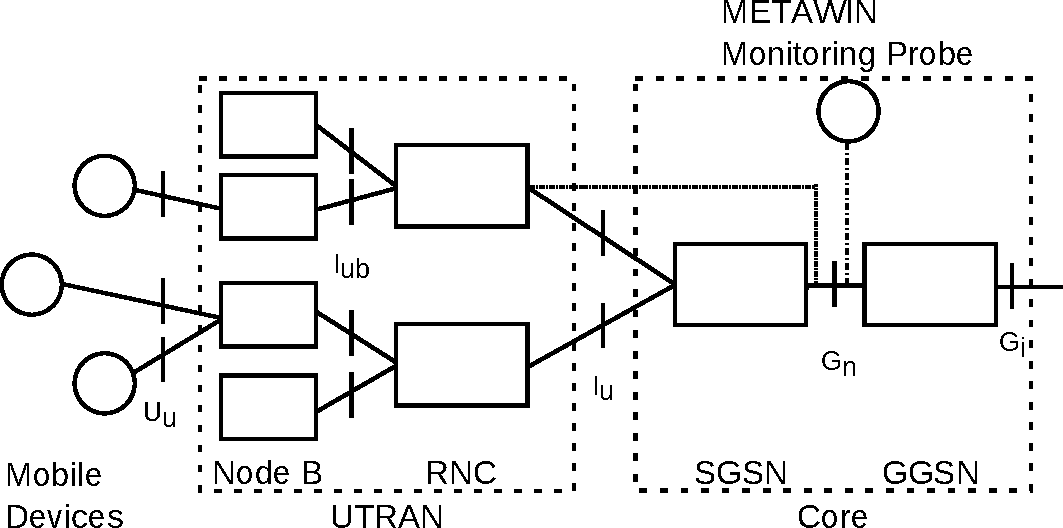
\includegraphics[width=0.7\textwidth]{images/umts-network.pdf}
	\caption{Location of the \acrshort{METAWIN} monitoring probe in the \acrshort{3G} core network.}
\label{c4:fig:umtsnetwork}
\end{figure}

The measurement taps are located at the Gn interface at one \gls{GGSN} within the core network as depicted in Figure~\ref{c4:fig:umtsnetwork}. It gives access to a wide spectrum of core \gls{gtp} signaling, including the mobility and tunnel management. The system does not offer a complete packet trace, but aggregates every signaling transaction and user traffic flow down to a number of select fields. This includes \gls{gtp} \gls{IE} such as the \gls{RAT} as well as the terminal types of the mobile clients. The latter is determinable by the \gls{TAC} part of the \gls{IMEI} and will be discussed later in detail.

In the network under study, a direct link between \glspl{GGSN} and the \glspl{RNC} and circumventing the \gls{SGSN} is present. It is only used for transporting user-plane traffic under specific circumstances, and signaling procedures are still carried out in the normal way between \glspl{SGSN} and \gls{GGSN}. Therefore, only the Gn interface at \gls{GGSN} is seeing the complete core network traffic, which explains the location of the tap. The network under study has more than one \gls{GGSN} at different physical locations. The tapped \gls{GGSN} manages about half of the operator's total traffic volume in this period. 

Recording data in a live network necessitates meeting strict privacy requirements regarding the handling of user-related data. \gls{METAWIN} complies with this by anonymizing all user-identifying. Application-level payload is removed and all user identifiers (e.g. \gls{IMSI}) are non-reversibly hashed before recording. \glspl{UE} in a dataset can still be differentiated by the hashes but not traced back to the actual user. The wiretaps deployed within the monitoring system are time-synchronized with \gls{GPS}. Accordingly, the packet timestamps have an accuracy of least \SI{100}{\nano\second}.


%%%%%%%%%%%%%%%%%%%%%%%%%%%%%%%%%%%%%%%%%%%%%%%%%%%%%%%%%%%%%%%%%%%%%%%%%%%%%%%%
\subsection{Dataset Description}

Using \gls{METAWIN} a week-long core trace was acquired. It was recorded in April 2011, specifically beginning at Monday, \yyyymmdddate\formatdate{10}{4}{2011}, \formattime{0}{0}{0} and ending Sunday, \formatdate{17}{4}{2011}, \formattime{23}{59}{59}.

The trace includes user plane as well as control plane traffic. User plane traffic is recorded in a traffic flow granularity with the trace containing data on \num{2.2e9} aggregated flows. No exact flow start time is given, instead it is rounded down to a \SI{2}{\hour} window with the timestamp at the beginning. A flow entry further consists of hashed identifiers for the gls{IMSI} and the remote server. Besides the usual protocol and port information, the transmitted data volume, in a number of packet as well as byte count, is given on in both link directions. Additional information is available on \gls{HTTP} traffic. This portion of the trace includes precise timestamps as well as the \acrshort{MIME}-type, result code, and size of the requested objected.

The recorded control plane traffic consists of \num{4.1e8} \gls{gtp} tunnel management transactions, i.e., every create, update, and delete request and response. Not all of the \glspl{IE} data is included. But most importantly, it includes the \gls{TAC}, \gls{RAT} and hashed \gls{IMSI} for the purpose of device discrimination. Also present are several timestamps with \SI{64}{\bit} precision describing the time of the request, response and the tunnel's start time. Finally, the \gls{gtp} data contains the response codes for each request. With these codes, failed transactions can be distinguished from successful ones and examined separately. Since the hashed \gls{IMEI} is consistent across the user and control plane data, both can be cross-correlated.

All trace information was exported from \gls{METAWIN} as pure line-based text data. For this investigation all records were fed into a \acrshort{SQL} database. Evaluations were conducted through scripted queries on the database using Python scripts and further statistically evaluated in R.

%%%%%%%%%%%%%%%%%%%%%%%%%%%%%%%%%%%%%%%%%%%%%%%%%%%%%%%%%%%%%%%%%%%%%%%%%%%%%%%
\subsection{Device Identification}

Individual device types in a mobile network can be identified in the data through the \gls{TAC} field on every entry. The \gls{TAC}, defined in \cite{3gpp.23.003}, represents the first eight decimal digits of the \gls{IMEI} and uniquely identifies each device type. The following six digits of the \gls{IMEI} constitute the serial number of a specific device, which is of course omitted in the data. Due to the short length of this serial number, popular devices will often be assigned more than one \gls{TAC}, somewhat complicating the identification of certain device models.

\glspl{TAC} are assigned to individual device models by the regional members, or \gls{RBI}, of the \gls{GSMA}, distinguished by the first two digits of the \gls{TAC}. The full allocation information is not freely available, but only to members of the \gls{GSMA}, which is not a viable option for research institutions and other interested parties. Some independent efforts have been made to collect \glspl{TAC} from devices. Most of them allow just low-volume queries for specific \glspl{TAC} for non-commercial purposes. However, one \gls{TAC} dataset is publicly available and can be used freely.\footnote{Available at: \url{http://www.mulliner.org/tacdb/}.}

This evaluation uses this dataset with some additional device identifiers and classification annotations collected during the course of the investigation. With this at hand, many of the devices associated with the flows and \gls{gtp} messages from the trace were iteratively identified and categorized.


%%%%%%%%%%%%%%%%%%%%%%%%%%%%%%%%%%%%%%%%%%%%%%%%%%%%%%%%%%%%%%%%%%%%%%%%%%%%%%%%
\subsection{\texorpdfstring{\acrshort{TAC}}{TAC} Evaluation Validity}

It is important to know whether the information available in the \gls{TAC} dataset covers enough of the devices seen in the traces to conduct sufficiently meaningful evaluations. After all, the \gls{TAC} data is large but might still be very incomplete due to the sheer number of devices in existence.

\begin{table}
\centering
\caption{Relative \acrshort{TAC} statistics.}
\label{c4:tbl:tacstats}
	\begin{tabu}{XX[r]}
		\toprule
		\textbf{Type} & \textbf{Relative number of devices with an entry in the \gls{TAC} dataset}\\ 
		\midrule
		Total number of flows & \SI{99.72}{\percent} \\
		Ratio of total traffic & \SI{99.97}{\percent} \\
		Total number of tunnels & \SI{87.57}{\percent} \\
		Total number of \gls{gtp} signaling messages & \SI{90.95}{\percent} \\
		Number of distinct \glspl{UE} & \SI{80.93}{\percent} \\ 
		\bottomrule
	\end{tabu}
\end{table}

Table~\ref{c4:tbl:tacstats} provides statistics on the devices that could be identified in the trace. About \SI{81}{\percent} of all unique \gls{TAC} present in the trace could be mapped to a known device. More importantly, when looking at the total number of tunnels and \gls{gtp} messages during the week, even \SI{91}{\percent} of the responsible device can be determined. Finally, the flow data shows an even clearer picture, as almost all of the devices involved can be identified.

This is an interesting result in itself, as the \SI{19}{\percent} of devices present in the dataset that could not be identified through the \gls{TAC} are the cause for only about \SI{9}{\percent} of signaling and \SI{0.3}{\percent} of total traffic. This means there is a long tail of device types in this mobile network with very little impact on the load. With these results, one can be rather confident that evaluations using device discrimination based on this \gls{TAC} mapping should give viable results.


%%%%%%%%%%%%%%%%%%%%%%%%%%%%%%%%%%%%%%%%%%%%%%%%%%%%%%%%%%%%%%%%%%%%%%%%%%%%%%%%
\subsection{Device Classification}

With these device-to-\glspl{TAC} mappings available, additional meta-information can now be added to it, intended to distinguish some of the described load influencing factors. Knowing the model gives also a good knowledge of the device's category and of the \gls{os} it is running by default.\footnote{The \gls{os} actually running on the device at the time of the measurement can not be inferred on this way. But the number of devices running a different \gls{os} than the one installed by default should be relatively low.}

The device's category represents a general classification of the device and should give some initial hints on the fields of use. The devices are partitioned into smartphones, feature phones, \gls{3G} USB dongles or \gls{3G}+WiFi routers, and all other devices. The term feature phone usually points at low-end mobile phones with at least some kind of data capability, often with a physical numerical keyboard. Phones, that could subjectively fall into either the smartphone or the feature phone category were generally attributed as smartphone. Not covered here are any kind of \gls{M2M} devices, because the \gls{TAC} mappings are very inconclusive and incomplete in this area.

The next classification variable is the \gls{os}. Most popular in the trace were the two dominant smartphone \glspl{os}, Android and iOS, and Symbian\footnote{While not completely accurate phones running Series 40 were also attributed to this category because of their close relationship.}, often found on feature phones. Other systems of note are Blackberry OS and Windows Phone or Windows Mobile, but they occur in such a low volume in the trace, that it was decided to completely neglect them and count them towards the other and unknown devices. It should also be noted, that USB dongles and routers cannot be linked to any specific \gls{os} solely by the knowledge of the \gls{TAC}. Also not distinguishable are the exact release versions of the \gls{os} on a specific device. This could diminish the evaluations, as the network behavior could change noticeably between two major versions.

With this knowledge, one can even conjecture on the applications running on the device. Combining the \gls{os} with lists of the most popular applications for this platform can already give some very helpful hints on what can be expected from the traffic mix these types of devices are generating. One final possible \gls{TAC} classification could be a categorization by the phone vendor. However, this was not conducted because it can be safely assumed that the impact is negligible in comparison to the device type and \gls{os}.


%%%%%%%%%%%%%%%%%%%%%%%%%%%%%%%%%%%%%%%%%%%%%%%%%%%%%%%%%%%%%%%%%%%%%%%%%%%%%%%%
\subsection{Preliminary Device Statistics}

After applying the categorization to the network dataset device composition was evaluated to get a first grasp of the network's makeup and to help understand the later investigations.

As expected, the two largest observed portions of devices are smartphones and \gls{3G} dongles, while classic feature phones do not seem to play a major role anymore. About twice as many Android as iOS devices are present, possibly attributed either to the contractual situation of the operator or the wider price range of Android devices.

Regarding traffic, feature phones have negligible user traffic despite still making up one tenth of the device fraction. The difference between \gls{3G} dongles and smartphones is also noteworthy. While the former cause large amounts of user plane traffic (compared to the device numbers), they are responsible for but a few core network signaling events and tunnels. This picture is reversed for smartphones.

One observation across all device types is that about \SI{14}{\percent} of all mobile devices have activated their \gls{GPRS} data service and \gls{gtp} tunnel and cause signaling traffic, but do not initiate any user plane traffic at all.


%%%%%%%%%%%%%%%%%%%%%%%%%%%%%%%%%%%%%%%%%%%%%%%%%%%%%%%%%%%%%%%%%%%%%%%%%%%%%%%
%!TEX root = ../../dissertation.tex
%%%%%%%%%%%%%%%%%%%%%%%%%%%%%%%%%%%%%%%%%%%%%%%%%%%%%%%%%%%%%%%%%%%%%%%%%%%%%%%%
\section{Statistical Methods}

As a final preparation for the evaluation all the statistical tools, that will be used in the evaluation, are briefly defined in this section with material based on \cite{field2012discovering} and \cite{Knuth:1997:ACP:270146}.


%%%%%%%%%%%%%%%%%%%%%%%%%%%%%%%%%%%%%%%%%%%%%%%%%%%%%%%%%%%%%%%%%%%%%%%%%%%%%%%%
\subsection{Distribution Functions and Fitting}

With a distribution function, also called \gls{CDF}, a monotonous mapping of continuous values to a probability can be well represented. It is defined as the probability that a random variable $X$ is less than or equal to a value $x$, or

\begin{equation}
	\phantom{.} F(x) = P(X\leq x)\text{.}
\end{equation}

Sample of real data are generally finite and not continuous. Hence, the distribution can only be approximated by an \gls{ECDF} $F_n(x)$ for values $X_1, X_2, \ldots , X_n$ and

\begin{equation}
	\phantom{.}F_n(x) = \frac{\text{number of }X_1, X_2, \ldots , X_i \leq x}{x}\text{.}
\end{equation}

One of the analysis's goal is to break down the actual measured system to a simplified probability model. This can be conducted by attempting to match the data's \gls{ECDF} to an existing basic probability distribution, e.g., exponential Gamma, log-normal, or Weibull. In order to achieve this one of several readily available matching methods, which rely either on closed formulas or numerical optimization, can be used. Two simple methods are \textbf{Matching Moments}~\cite[pp.~99-143]{vose2000risk} and \textbf{Maximum Likelihood}.

The former estimates parameters for a preselected distribution functions by optimizing the target distribution function to converge its moments to that of the sample data. The latter approach finds a fitting target probability function by calculating the log-likelihood of the data for a preselected distribution and maximizing the likelihood.

In such cases where none of the basic probability distributions proved to be a good fit an attempt was made to converge rational functions to the sample \gls{ECDF} with an optimization tool specialized for this case, Eureqa~\cite{eureqa_software, eureqa_paper}. While not as good as a simple model with a probability distribution, having a rational function as a description for a dataset can enable some further statistical and queuing theoretic evaluation.


%%%%%%%%%%%%%%%%%%%%%%%%%%%%%%%%%%%%%%%%%%%%%%%%%%%%%%%%%%%%%%%%%%%%%%%%%%%%%%%%
\subsection{Statistical Tests}

To check the statistical goodness of the generated fits, statistical tests can be used. Generally, tests compare the values observed in an experiment to expected values following a theoretical distribution. In this case, the tests are used to validate and estimate the quality of the discovered fits to the empirical data.

First, as a simple measure, the \textbf{Pearson correlation coefficient} can be facilitated, comparing the covariance and standard deviation of the empirical and fitted variables. Another possible approach is \textbf{Pearson's $\chi^2$ test for independence}~\cite{doi:10.1080/14786440009463897}, which is the oldest known test and defined as

\begin{equation}
	\phantom{.}V=\sum_{i=1}^{k} \frac{{(o_i - e_i)}^2}{e_i}\text{.}
\end{equation}

This simply calculates the sum of the squared difference between the observed $o_i$ an expected values $e_i$ and adjusts each for their weight. The result can then be compared to the $\chi^2$-distribution with the same degrees of freedom
%\footnote{The degree of freedom of count experiments is one less than the number of observable categories.}
as the test for a given significance level. In most practical cases this comparison is conducted against precomputed tables with set significance levels. The data collected in this thesis is typically continuous in nature on which this test cannot be used directly. However, data could still be split into a finite number of intervals, as is done when generating a histogram, and then using the intervals as categories for the $\chi^2$ test, albeit with a certain loss of precision.

Continuous data can be checked with the \textbf{Kolmogorov-Smirnov test}. First suggested by Kolmogorov in 1933~\cite{kolmogorov1933sulla} and expanded on by Smirnov in 1939~\cite{smirnov1939estimation} it is defined as

\begin{align}
	K_n^+ &= \sqrt{n} \sup_{-\infty < x < + \infty} \left( F_n(x) - F(x) \right) \\
	\shortintertext{and}
	\phantom{,}K_n^- &= \sqrt{n} \sup_{-\infty < x < + \infty} \left( F(x) - F_n(x) \right)\text{,}
\end{align}
%
for the \gls{ECDF} $F_n(x)$ and \gls{CDF} $F(x)$. Once again the results are compared against a precomputed table of values from the Kolmogorov-Smirnov distribution to test the significance of the observed results' deviation from expected values. 

Finally, every fit should in addition always undergo a \textbf{Visual Inspection}. Diagrams, of the empirical and fitted distribution --- especially histograms, density, and \gls{CDF} --- should be compared and checked for specific artifacts or outliers. 



%%%%%%%%%%%%%%%%%%%%%%%%%%%%%%%%%%%%%%%%%%%%%%%%%%%%%%%%%%%%%%%%%%%%%%%%%%%%%%%%
\subsection{Random Sampling}

Most of the evaluations in Section~\ref{c4:sec:evaluations} use random sampling to work on a subset of the original data.  Not only does this simplify the handling of a dataset this large sets --- working on a set with two billion entries can be quite problematic --- but can even improve statistical significance, as rare outliers tend to get removed by drawing samples. By selecting entries using a uniform distribution it is ensured that no unintentional sampling bias occurs. The intended evaluation is now applied onto multiple and independently drawn sample groups. If the results of every sample agree then it is also highly likely that the assumption holds for the whole data set.




%http://cran.r-project.org/web/packages/fitdistrplus/fitdistrplus.pdf





%%%%%%%%%%%%%%%%%%%%%%%%%%%%%%%%%%%%%%%%%%%%%%%%%%%%%%%%%%%%%%%%%%%%%%%%%%%%%%%
%!TEX root = ../../dissertation.tex
%%%%%%%%%%%%%%%%%%%%%%%%%%%%%%%%%%%%%%%%%%%%%%%%%%%%%%%%%%%%%%%%%%%%%%%%%%%%%%%%
\section{Mobile Core Signaling Evaluation}
\label{c4:sec:evaluations}

Finally, the core network control plane load evaluations can now be tackled. The previously described dataset is thoroughly investigated several approaches to measure load and related factors are iterated.


%%%%%%%%%%%%%%%%%%%%%%%%%%%%%%%%%%%%%%%%%%%%%%%%%%%%%%%%%%%%%%%%%%%%%%%%%%%%%%%%
\subsection{Traffic Ratio Estimations}

\begin{table}
\centering
\caption{Relative device-discriminated traffic statistics extracted from the dataset.}
\label{tab:trafficstats}
	\begin{tabu}{X[1.4]X[r]X[r]X[r]X[r]X[r]}
	\toprule
	& \textbf{Flows} & \textbf{Traffic} & \textbf{Tunnels} & \textbf{\gls{gtp} messages} & \textbf{Devices}\\ 
	\midrule
	\multicolumn{2}{c}{\textbf{By device type}}       &             &             &             &           \\
	% In TAC DB      & $99.72\%$   & $99.97\%$   & $87.57\%$   & $90.95\%$   & $80.93\%$ \\
	Smartphones      & $20.58\%$   & $12.81\%$   & $60.31\%$   & $75.99\%$   & $37.97\%$ \\
	Regular phones   & $0.26\%$    & $0.37\%$    & $5.40\%$    & $0.94\%$    & $9.25\%$  \\
	\gls{3G} dongles & $66.55\%$   & $75.12\%$   & $12.71\%$   & $9.53\%$    & $25.10\%$ \\
	\midrule
	\multicolumn{2}{c}{\textbf{By \gls{os}}}       &             &             &             &           \\
	Android          & $10.82\%$   & $6.48\%$    & $14.33\%$   & $43.33\%$   & $14.01\%$ \\
	iOS              & $7.22\%$    & $4.47\%$    & $18.91\%$   & $20.35\%$   & $7.94\%$  \\
	Symbian          & $1.02\%$    & $1.09\%$    & $21.17\%$   & $4.51\%$    & $12.97\%$ \\
	Blackberry OS    & $0.07\%$    & $0.10\%$    & $2.17\%$    & $2.60\%$    & $1.48\%$  \\
	\bottomrule
	\end{tabu}
\end{table}

To get a first grasp of the dynamics present in the dataset and the core network under investigation, Table~\ref{tab:trafficstats} shows a small survey of the traffic composition split up by device type and \gls{os} categories. The majority of signaling messages originated from smartphones, which in turn generated only a small portion of user traffic when compared to \gls{3G} dongles.

With these numbers, the notion of active devices or tunnels can also be introduced. This only includes entities that, besides signaling, actively generated user traffic during their life cycle. Interestingly, only about \SI{82}{\percent} of all unique devices in the trace were active and could be associated with at least one traffic flow. The remaining \SI{18}{\percent} of devices still had an open \gls{gtp} tunnel but never used it. This is an extreme for the core network, as it causes a significant amount of control plane load without any actual benefit to either the network or the device. The active device distinction will also be used later on in the evaluation.

Unfortunately, the dataset does not contain any hard numbers on the volume of the signaling messages, which could be a direct indicator of the network load the control plane imposes. But using the estimation of the upper limit of a \gls{gtp} message from Section~\ref{c4:sec:gtp}, a rough upper limit on the total signaling traffic can also be derived. The following formula is used:

\begin{align}
	\phantom{,}v_s &= 2\left|S\right|(v_{gtp} + v_{udp} + v_{ip})\text{,}\\
	\phantom{.}t_r &= \frac{v_s}{v_t} \approx 0.7\si{\percent}\text{,}
\end{align}
%
with the signaling volume $v_s$, the set of signaling messages $S$, the estimated size of a \gls{gtp} message $v_s$, and the length of the \gls{UDP} and \gls{IP} headers. In this scenario, the traffic ratio $t_r$ of $v_s$ compared to the total traffic $v_t$ is calculated to be a minute \SI{0.7}{\percent}. Therefore, it can be safely assumed that the volume of control plane traffic appears to be a non-issue and not the bottleneck. The other load factors at the network nodes described earlier must play a more critical role, such as the memory profile of the states kept in the gateway nodes, the time required to process the large number of information held in the messages, or the imposed latency through several message round trips during transactions.

This is why the following evaluations are all intended to find some indirect approach to measure the system's load.



%%%%%%%%%%%%%%%%%%%%%%%%%%%%%%%%%%%%%%%%%%%%%%%%%%%%%%%%%%%%%%%%%%%%%%%%%%%%%%%%
\subsubsection{\texorpdfstring{\acrshort{gtp}}{GTP} Tunnel Duration}

The first indirect evaluation target will be the duration of the \gls{gtp} tunnels. This duration is directly related to the amount of occurring tunnel management signaling between the \gls{SGSN} and \gls{GGSN}. In turn, each of these signaling interactions causes processing at the two involved nodes and changes the amount of state in the form of the \gls{PDP} context. In terms of signaling messages, looking at the duration catches both tunnel create and delete messages, but no update message.

For the purpose of the evaluation the duration is defined as the interval between corresponding \gls{gtp} create and delete messages. As soon as the \gls{GGSN} sends its successful response to the create request, it can be expected that the necessary state has been created throughout the \gls{CN} and is ready to forward user packets. Similarly, after a delete message, user traffic should not be forwarded anymore. However, state may still exist and could be freed up lazily. But the latter depends entirely on the specific implementation.

As a side note, while the trace itself is only one week long, information on tunnels longer than this period can still be obtain when they were closed during the period. The trace's record on delete messages also contains the timestamp of the initial tunnel creation.

All the individual tunnel durations in the dataset are differentiated based on two factors based on the presented \gls{TAC} mechanics. The first part of the investigation looks at tunnels from different device types. After that, possible influences from the operating system are investigated. 


%%
\paragraph{Influence of the Device Type}

\begin{figure}[htb]
	\centering
	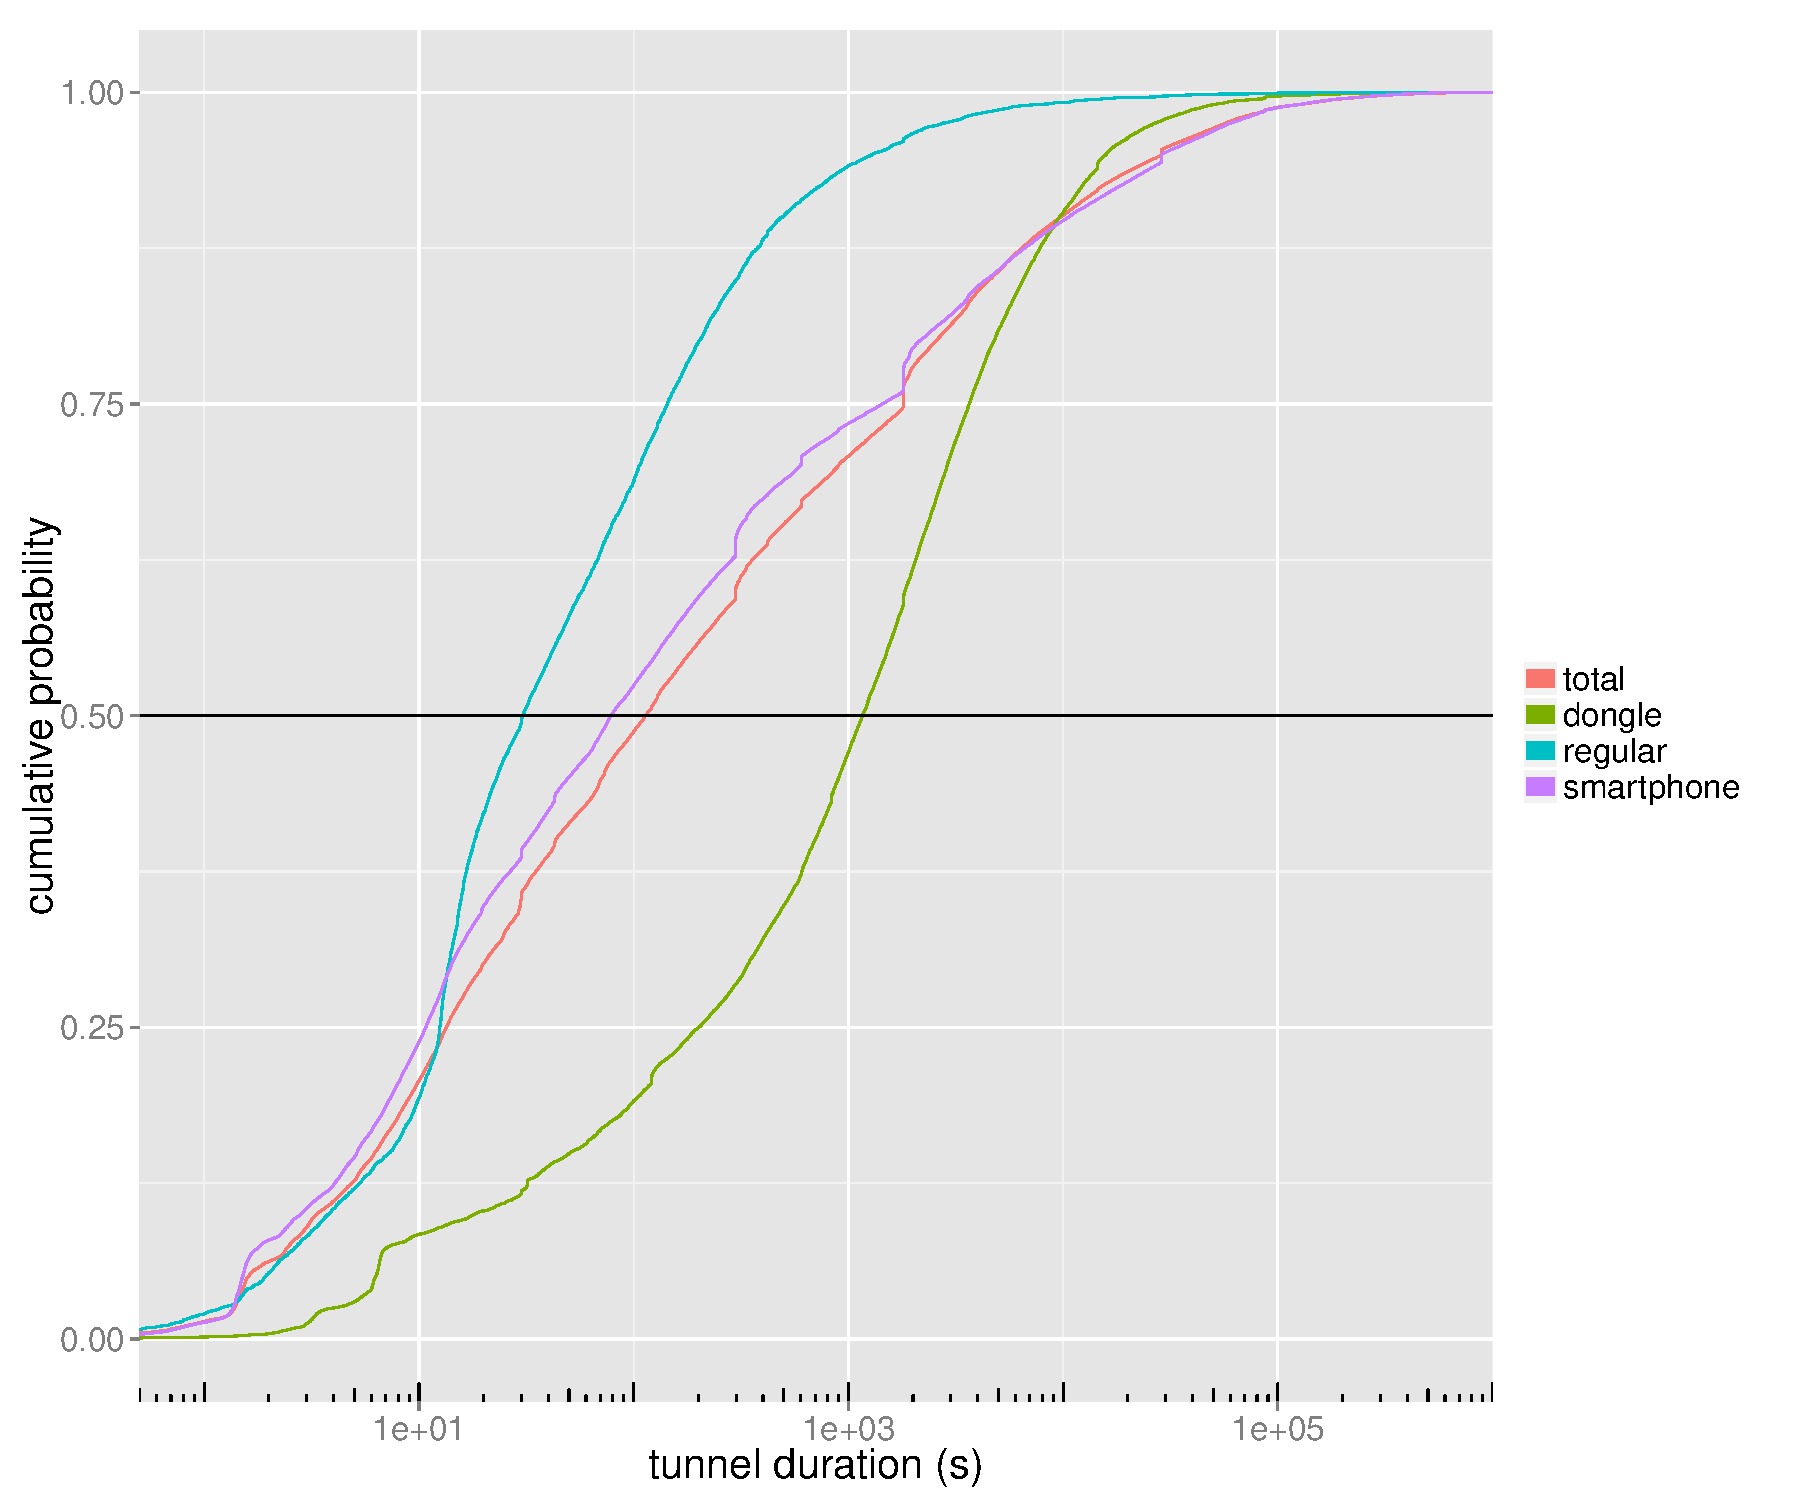
\includegraphics[width=0.9\textwidth]{images/R-tunnel-duration-device-type.pdf}
	\caption{Tunnel duration distribution, separated for \acrshort{3G} dongles, smartphones and regular phones with medians at \SI{115}{\second} (total), \SI{31}{\second} (regular), \SI{82}{\second} (smartphone), and \SI{1207}{\second} (dongle).}
\label{c4:fig:cdf-duration-device-class}
\end{figure}

Figure~\ref{c4:fig:cdf-duration-device-class} shows the \gls{ECDF} for the user tunnels and their \gls{PDP} Context durations in the dataset. In this first graph, the duration of different device classes is distinguished and put in perspective to the overall duration distribution. The devices classes here are smartphones, regular phones, and \gls{3G} dongles. It can be observed that tunnel durations range between seconds and more than one week.

The median can be clearly differentiated between device types, being much longer for \gls{3G} dongles than for mobile phones. This reflects expected user behavior very well and gives a first indicator on a possible influence of the user plane on the control plane.

Dongles are usually used with laptops to be able to work while being mobile. Dongle sessions last therefore often for extended periods longer than a few minutes up to hours. Also, this type of device is usually put into a standby mode after the period, which completely disables any mobile connections --- and therefore any associated tunnel --- instead of switching to low power radio idle modes. This is reflected in the dongle tunnel duration here as well. When compared to the other device category, dongles are more compactly centered around their median of about \SI{20}{\minute}.

A similar behavior can be observed in the regular phone distribution with values arranged tightly around the median of \SI{31}{\second}. Compared to today's smartphones, data connections on regular phones are mostly initiated explicitly by user interaction, for example through starting a browser and viewing a web page. This could also explain the comparatively low durations here.

The picture is rather different in the smartphone tunnel duration. Here, often background tasks are running over long periods of time and devices try to keep connectivity up as long as possible (while still attempting to conserve power). Overall, this could lead to the smoother distribution seen here with no clear center value.

Overall, a relatively high number of tunnels with a duration shorter than \SI{10}{\second} can also be observed. Especially the peak at about \SI{1.5}{\second} --- which is interestingly shifted to \SI{6.8}{\second} in the dongle distribution --- is of note. This is even shorter than the default values for the \gls{RRC} idle state transitions which causes the tunnel to be destroyed. It can be conjectured that these short tunnels have been explicitly removed by the \gls{UE} as no other involved state machine has timers this short.

Another distinct step at \SI{30}{\minute} in the total and smartphone distributions can be observed. As it is only present in these to categories --- and the total distribution looks to be mostly governed by smartphones --- it is reasonable to assume that the cause for this is a specific behavior observable in some aspect of smartphone related influence factors.


%%
\paragraph{Influence of the \texorpdfstring{\acrshort{os}}{OS}}

\begin{figure}[htb]
	\centering
	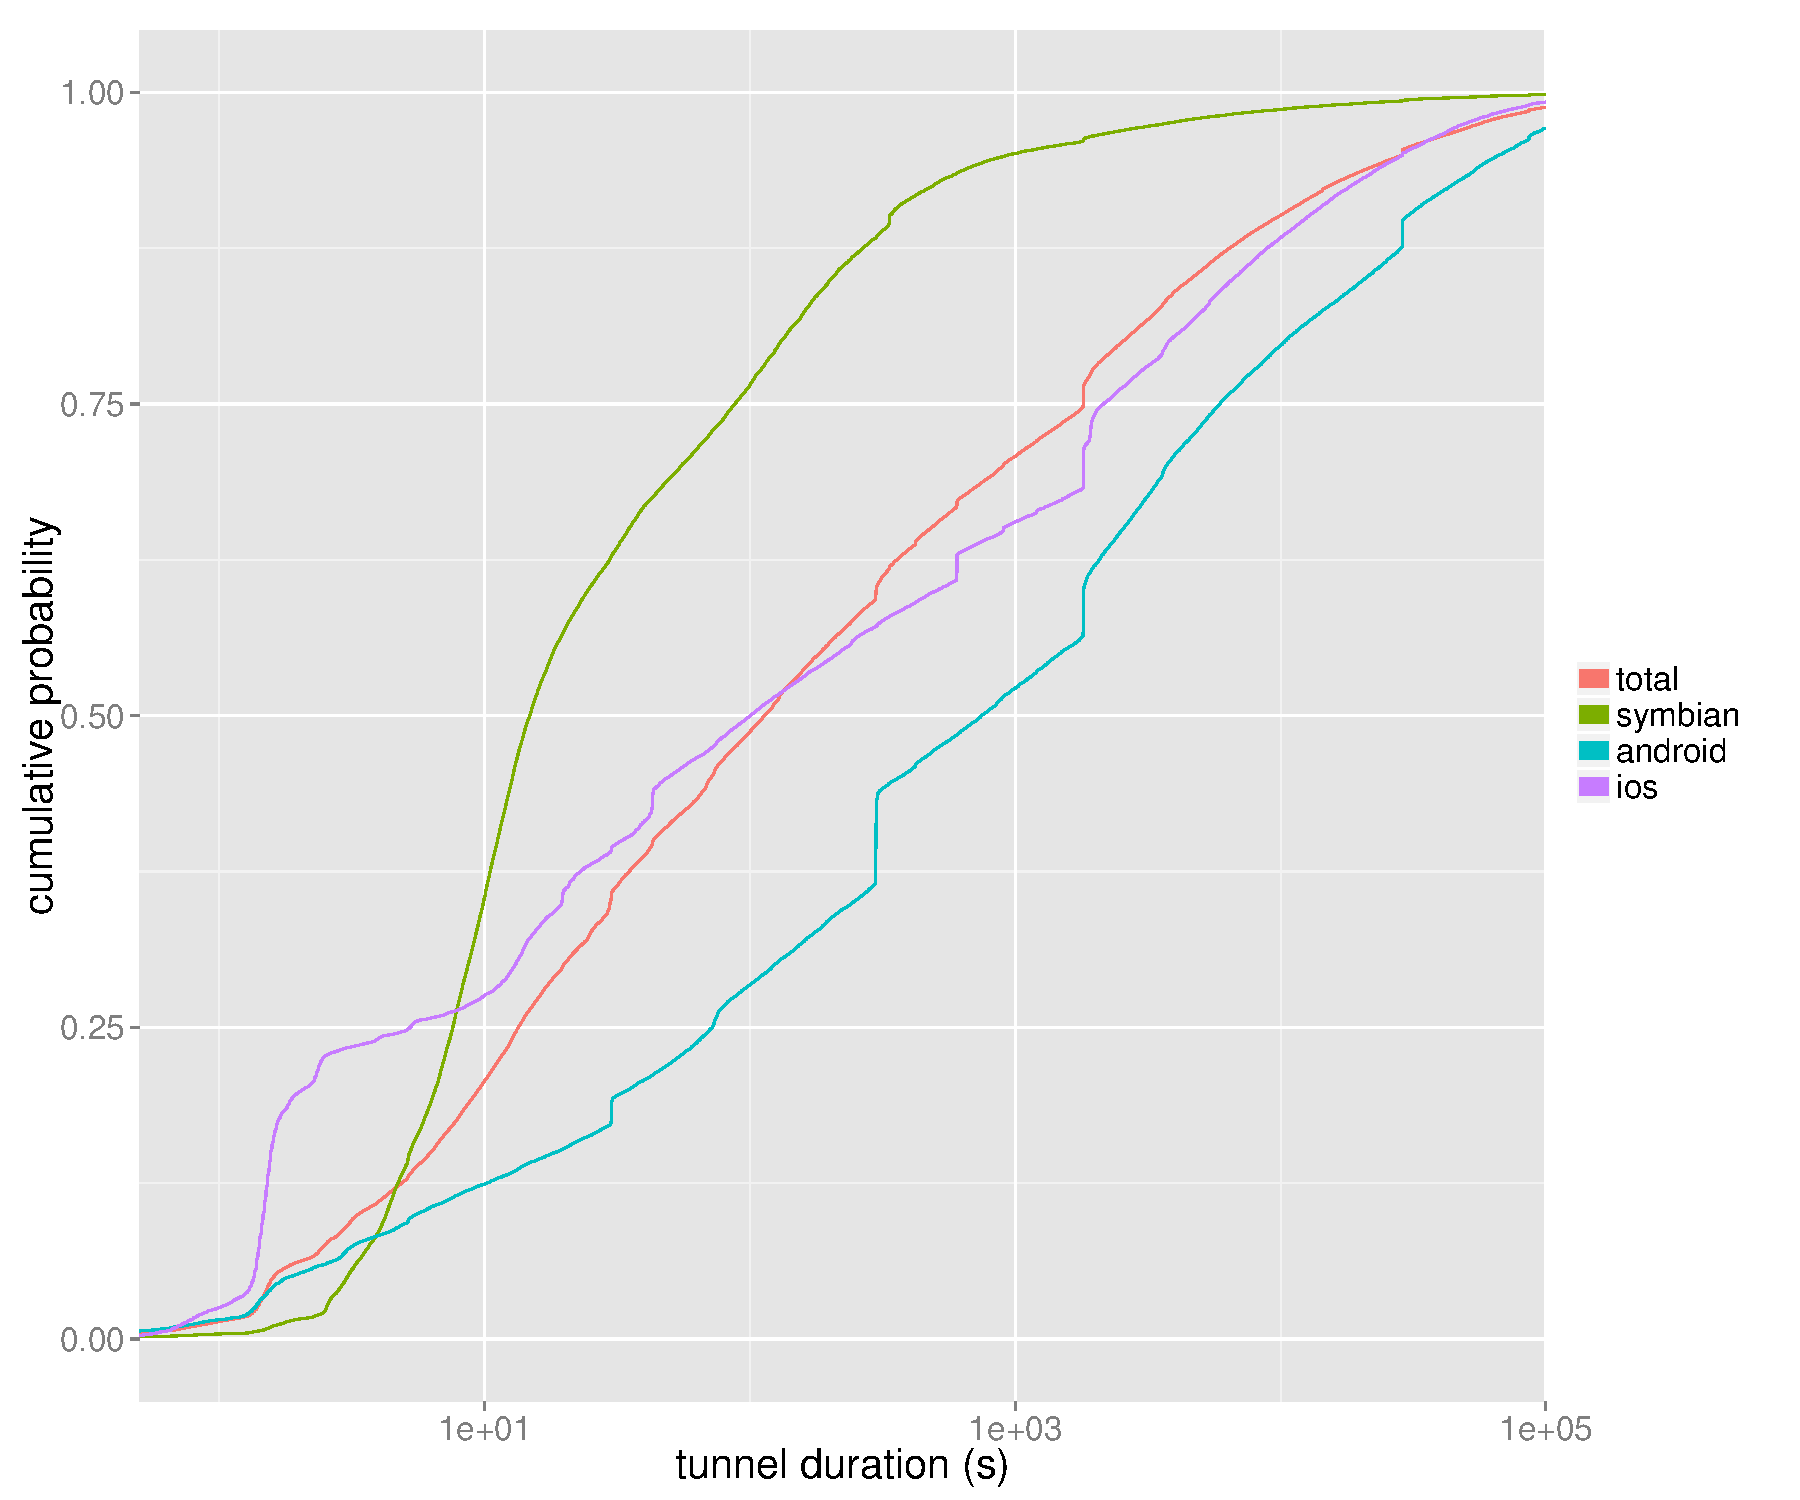
\includegraphics[width=0.9\textwidth]{images/R-tunnel-duration-operating-system.pdf}
	\caption{Tunnel duration \acrshort{CDF}, separated for select \acrshortpl{os}; Medians at \SI{115}{\second} (total), \SI{15.5}{\second} (symbian), \SI{104}{\second} (iOS), and \SI{765}{\second} (android).}
\label{c4:fig:cdf-duration-os}
\end{figure}

Next, the two phone categories are further broken down by their \gls{os}. Only the three major systems, Android, iOS, and Symbian, are identified here, the amount of other types was negligible. The smartphone category is almost exclusively represented by Android and iOS devices, while Symbian devices make up most of the regular phones but is also represented in a number of smartphone models.

Figure~\ref{c4:fig:cdf-duration-os} depicts the \gls{ECDF} of the tunnel durations of these categories in relation to the total duration distribution. They immediately exhibit a clear difference between individual \glspl{os}.

The Symbian tunnel durations are similarly distributed to the previously depicted regular phone category, albeit with an even shorter duration median of about \SI{15}{\second}. This is an indicator of the large intersection between these two groups and the explicit user traffic property attributed to regular phones.

The two smartphone-exclusive \gls{os} have remarkably similar tunnel distributions with the exception of the Android tunnel distribution shifted to much longer tunnels. This is mostly due to the larger accumulation of iOS tunnels around the previously mentioned \SI{1.5}{\second} mark. Over \SI{20}{\percent} of all tunnels established by iOS devices are shorter than \SI{2}{\second}. A possible explanation is an interaction between the described implicit background traffic happening in intervals and the efforts of iOS phones to preserve as much energy as possible. 

To this end, phones aggressively force their radio connection to the low power idle states or even completely shut off the radio immediately after transmission have ended, circumventing \gls{RRC} timers. To achieve this, iOS devices are known to implement a form of \gls{3GPP} Fast Dormancy~\cite{gsma2011fdbestpract}. It is deemed to improve device battery life, radio signaling and radio spectrum efficiency. Due the more frequent state transitions it also could cause an increase in core network tunnel management signaling, which is probably what happened in the iOS case depicted in the \gls{ECDF}.

Another set of tunnel duration accumulations are also visible in the \gls{os} distributions. Two types of steps should be distinguished here. First are accumulations that occur across multiple or all categories. This points to an influence source outside of the specific category. If the artifact is present in every distribution it is even likely that the source is a behavior of the network's state machines. The second type of accumulation is local to one or some categories, which places the root cause into the region of these categories and their related influence factors. 

In case of the \gls{os} category, additionally, peaks at \SI{30}{\second}, \SI{300}{\second}, and \SI{600}{\second} can be observed. However, whether this behavior can be attributed directly to the operating systems themselves cannot be decided just by looking at these distribution. Other factors, e.g., the device's baseband and user traffic dynamics, also play a role. 


%%
\paragraph{Influence of the Time of Day}

\begin{figure}[htb]
	\centering
	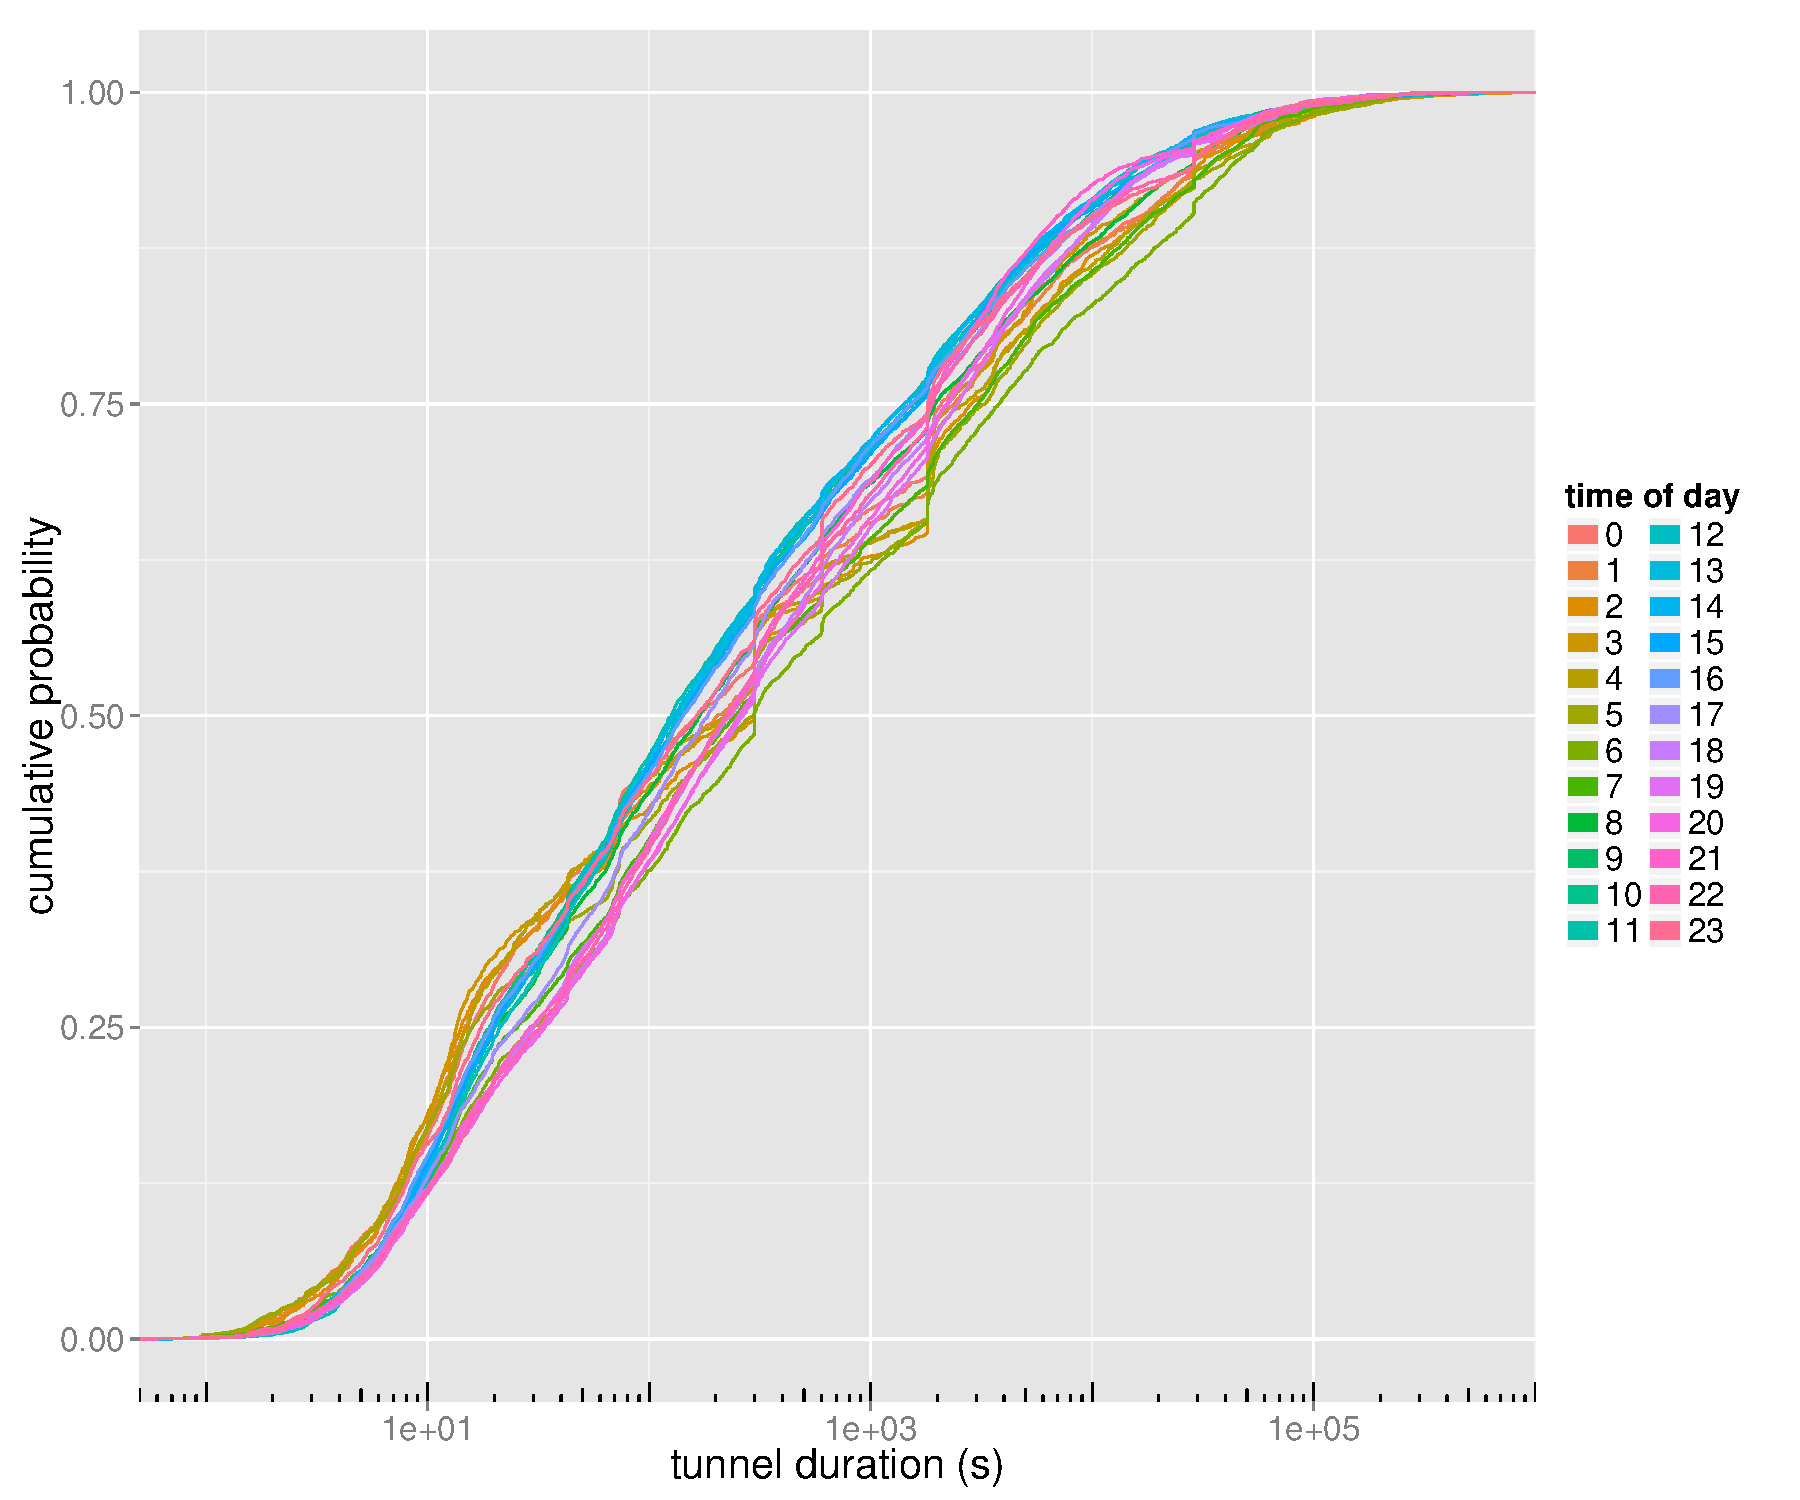
\includegraphics[width=0.9\textwidth]{images/R-duration-timeofday-ecdf.pdf}
	\caption{Tunnel duration of all active tunnels by time of day.}
\label{c4:fig:duration-timeofday-ecdf}
\end{figure}

In addition to device factors, diurnal effects could also play a role in the duration of tunnels. Figure~\ref{c4:fig:duration-timeofday-ecdf} depicts $24$ individual \glspl{ECDF} of the tunnel duration for each hour of a day. While no clear distinctions are visible, there is a trendto shorter tunnels in the early morning hours. The early afternoon hours tend to produce tunnels more centered around the middle duration range. Even longer tunnels should be treated with reservation, as they exceed the length of their assigned time slot in the \gls{ECDF} and span a larger time frame. Only the tunnel creation point is guaranteed to be in the slot.


%%
\paragraph{Influence of Other Factors}

Due to the nature of the trace dataset at hand many other influence factors are hard or outright impossible to distinguish. Some factors are unknown from the \gls{CN} perspective, as the mentioned device baseband, while others have not been recorded in the trace.

For example, it would theoretically be possible to investigate the influence of the \gls{RAT} as it is an \gls{IE} in the \gls{gtp} messages and also recorded in the trace. The radio access parts of \gls{GSM} and \gls{UMTS} are completely different --- including the \gls{RRC} state machines which were depicted in Figure~\ref{c4:fig:mmstatemodel} --- and therefore could also differ in their control plane load impact on the core. However, the \gls{RAT} \gls{IE} is optional and only set in less than \SI{1}{\percent} of the available records. As the radio access can change even during an existing tunnel --- in which case the \gls{GGSN} receives a \gls{gtp} update request informing the node about the change --- a complete picture without gaps would be required to do any investigation on this.


%%
\paragraph{Influence Strength of the Categories}

\begin{figure}[htb]
	\centering
	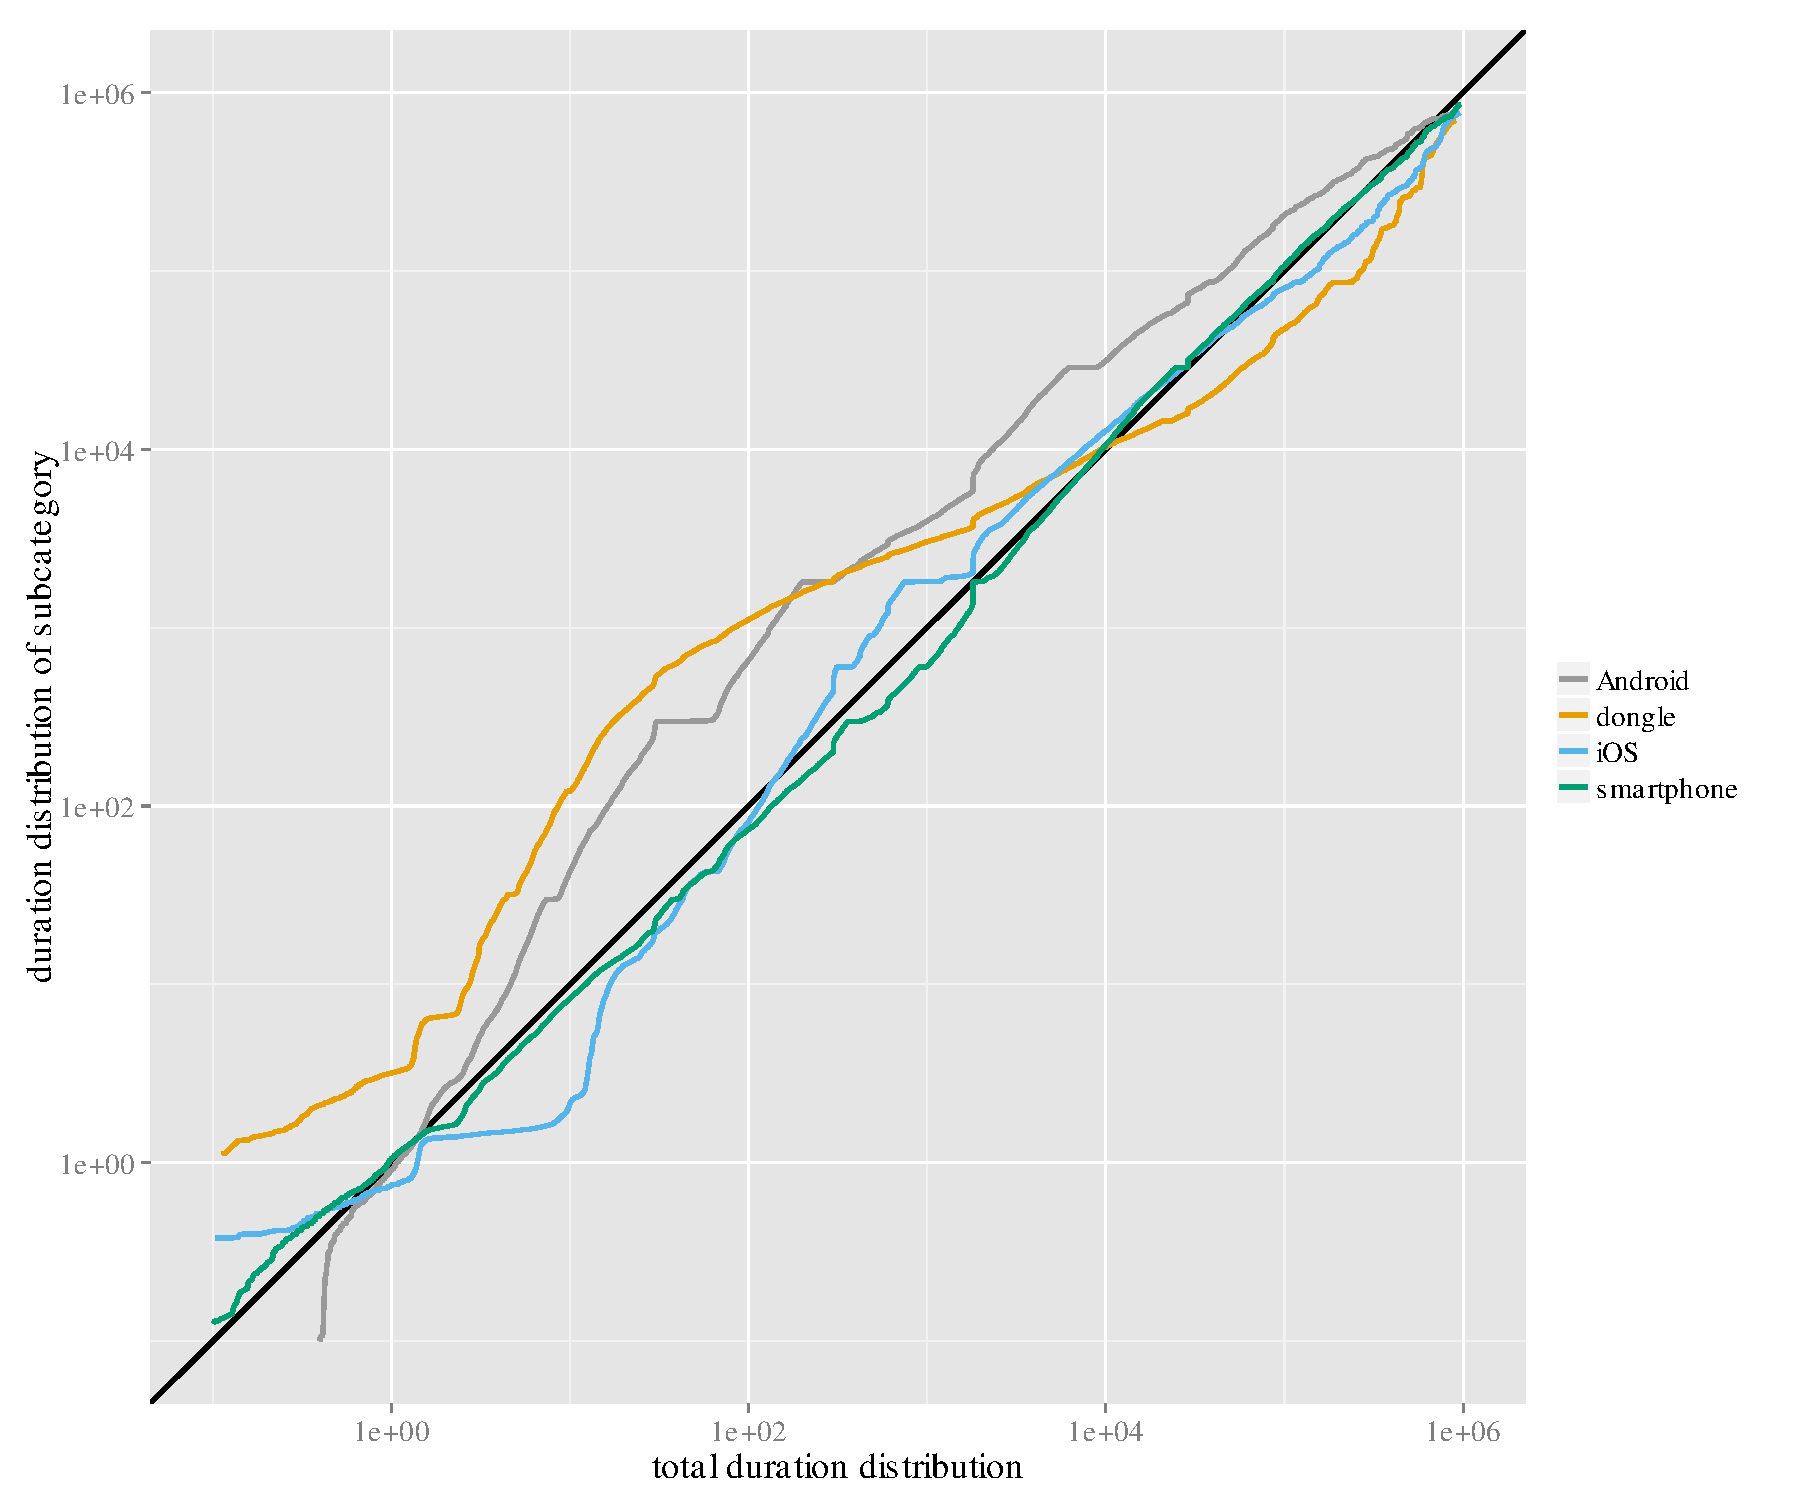
\includegraphics[width=0.9\textwidth]{images/R-duration-qq-category-comparison.pdf}
	\caption{Q-Q Plots of the tunnel duration distributions in comparison to device classification categories.}
\label{c4:fig:qq-plots}
\end{figure}


To ascertain which of the investigated device categories influences the total duration distribution most, Q-Q plots are created and investigated. It is conjectured that the amount of influence on the duration distribution is correlated to the influence on the control plane load. In theory, if both durations follow the same distribution, one expects a straight diagonal $y=x$ line through the origin. A steeper incline indicates more compact regions in the distribution plotted on the $x$ axis and vice versa.

The Q-Q plots in Figure~\ref{c4:fig:qq-plots} compare the total tunnel duration distribution to the duration distribution of the dongle, smartphone, Android, and iOS classification cateogries. It can be observed that the smartphone duration distribution is distributed almost equally to the total except for minor variations. However, the \gls{3G} dongle tunnel durations follow a very different distribution. Their effect on the total duration distribution seems to be negligible despite the  large amount of traffic they are causing. This is also a first indicator that smartphones might have a larger impact on signaling than other device types.

Looking closer at the smartphone category, Q-Q plots of the two major \glspl{os} are investigated. With the exception of the large below \SI{2}{\second} peak in the lower tail of the distribution, iOS device tunnel durations are very similar to the overall tunnel duration distribution. The same can not be said about the Android distribution, which deviates somewhat in the distribution's center but is similar to the total distribution in the upper tail. Even devices with just a different \glspl{os} seem to strongly differ in their influence on duration distribution and therefore on signaling.

\begin{figure}[htb]
	\centering
	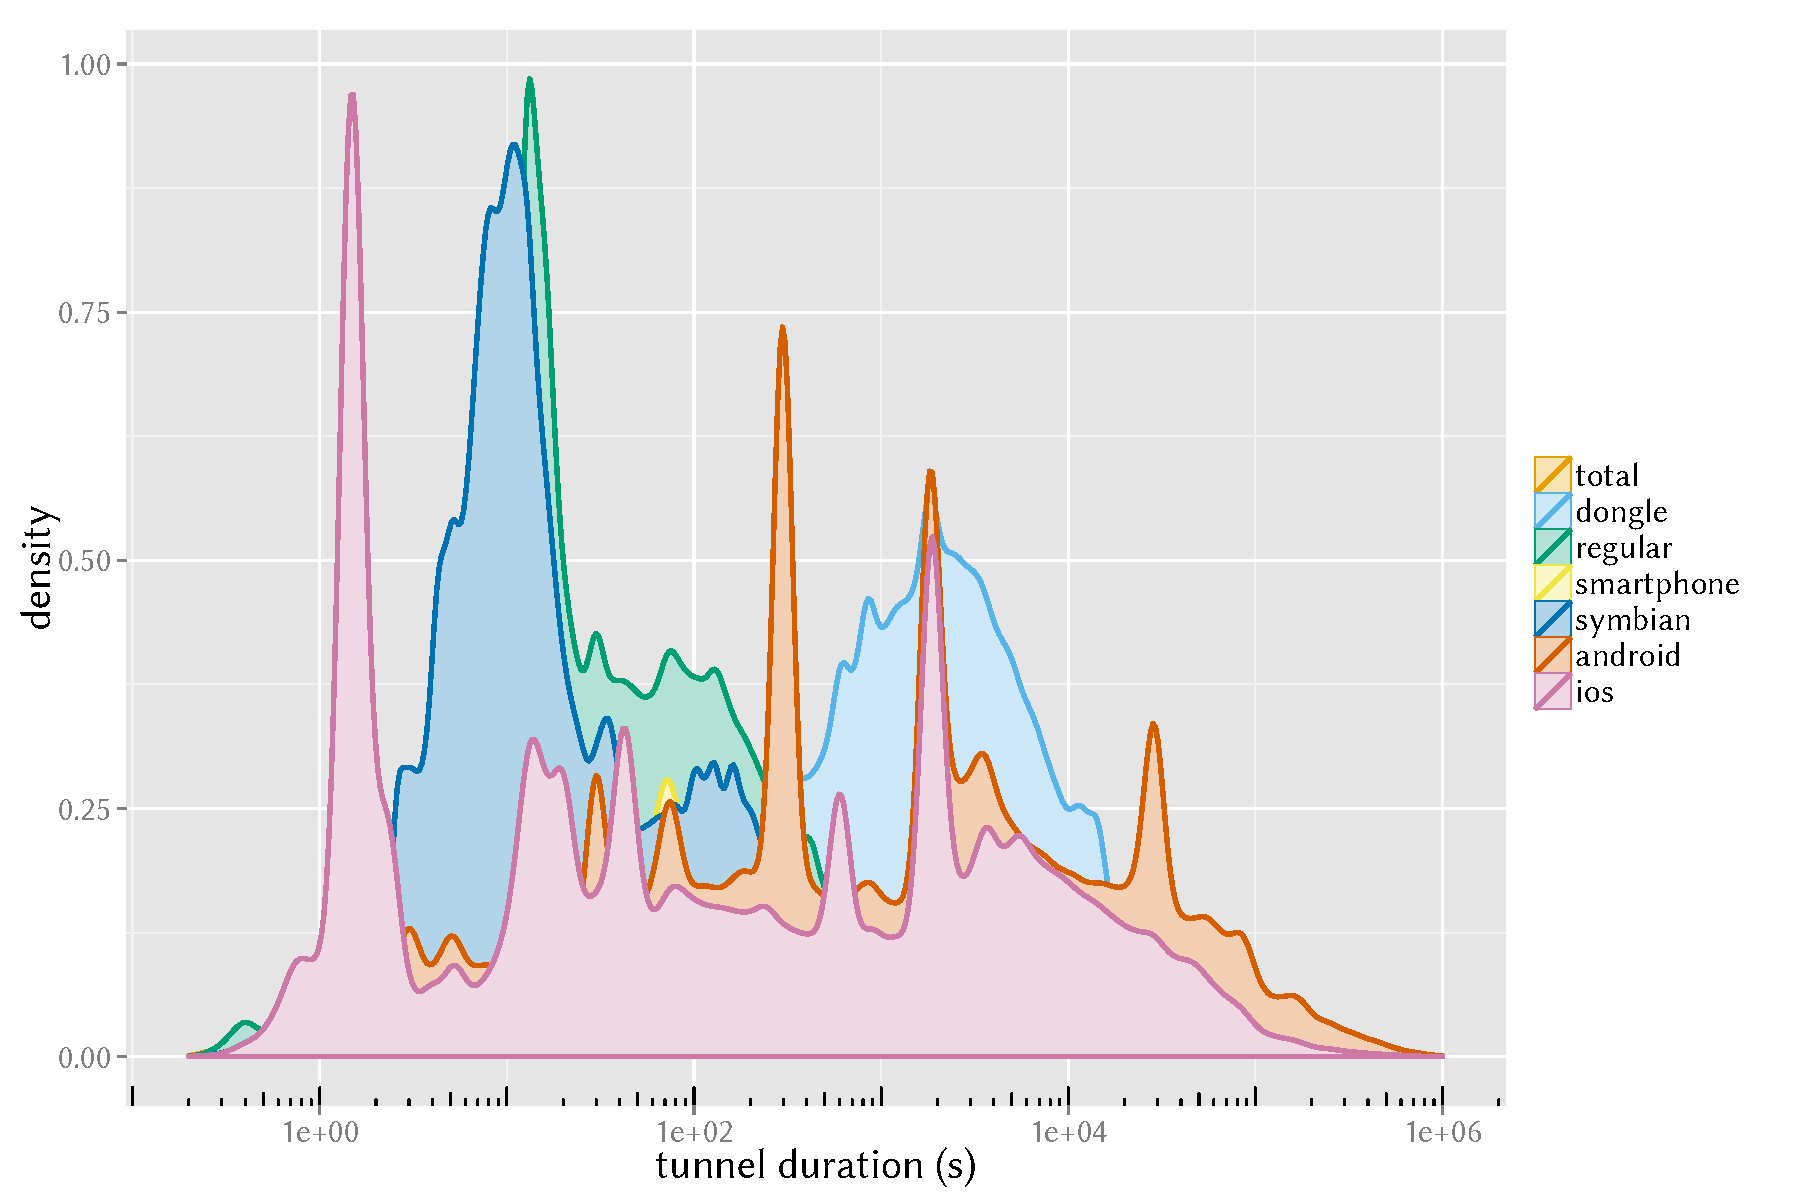
\includegraphics[width=0.9\textwidth]{images/R-duration-classification-density.pdf}
	\caption{Logscale density plot of the tunnel duration with all classifications.}
\label{c4:fig:durations-density}
\end{figure}


Figure~\ref{c4:fig:durations-density} attempts to depict where in their distributions the investigated device categories show the most impact on the total distribution. The plot shows the density of all previously investigated device influence categories.

It is evident that the durations are not evenly distributed, but rather follow sharp spikes. One of largest spike across all categories is the one at a duration of \SI{30}{\minute}, with about \SI{1.8}{\percent} of all tunnels in the network falling into that region. Since this spike happens across all device types, it makes a rather strong case for being induced by the network. On the other hand, the bulk of tunnel durations in the short-to-medium range does not seem to be governed by the two major smartphone operation systems but by other devices in the network, which do not show major spikes in other bins.

Besides the long-tailed behavior in the upper tail of the tunnel durations another slight accumulation effect, repeating itself every \SIrange{6}{7}{\day}, is present in the upper tail. This phenomenon is as yet of unknown origin and does not coincide with any known timers of the \gls{3G} mobile network.

The investigation of this data leads to the conclusion that the planning and dimensioning of the control plane needs to watch the behavior of smartphones more carefully than that device types.


%%%%%%%%%%%%%%%%%%%%%%%%%%%%%%%%%%%%%%%%%%%%%%%%%%%%%%%%%%%%%%%%%%%%%%%%%%%%%%%
\subsubsection{\texorpdfstring{\acrshort{gtp}}{GTP} Tunnel Arrivals}

The duration of \gls{gtp} tunnels is but one aspect of influence on control plane load. The arrival process of these tunnels is also interesting in itself. Specifically, this mean the arrival of tunnel requests, i.e.\gls{gtp} create requests, at the \gls{GGSN}. 

An arrival process can be described in two distinct ways. First by the number of arrivals in a given time interval. Second, by the \gls{IAT}, the time between two consecutive tunnel arrivals. Depending on the choice one has to deal with either a discrete or a continuous distribution.

Here, the tunnel arrival process is investigated with both approaches. This also adds to the foundation of the load model constructed in the next chapter. Note, that the notion of classifying arrivals into influence categories based on device specifics is omitted here. An investigation of this process can not be realistically be conducted categorized and still relate to the total system load.

\begin{figure}[htb]
	\centering
	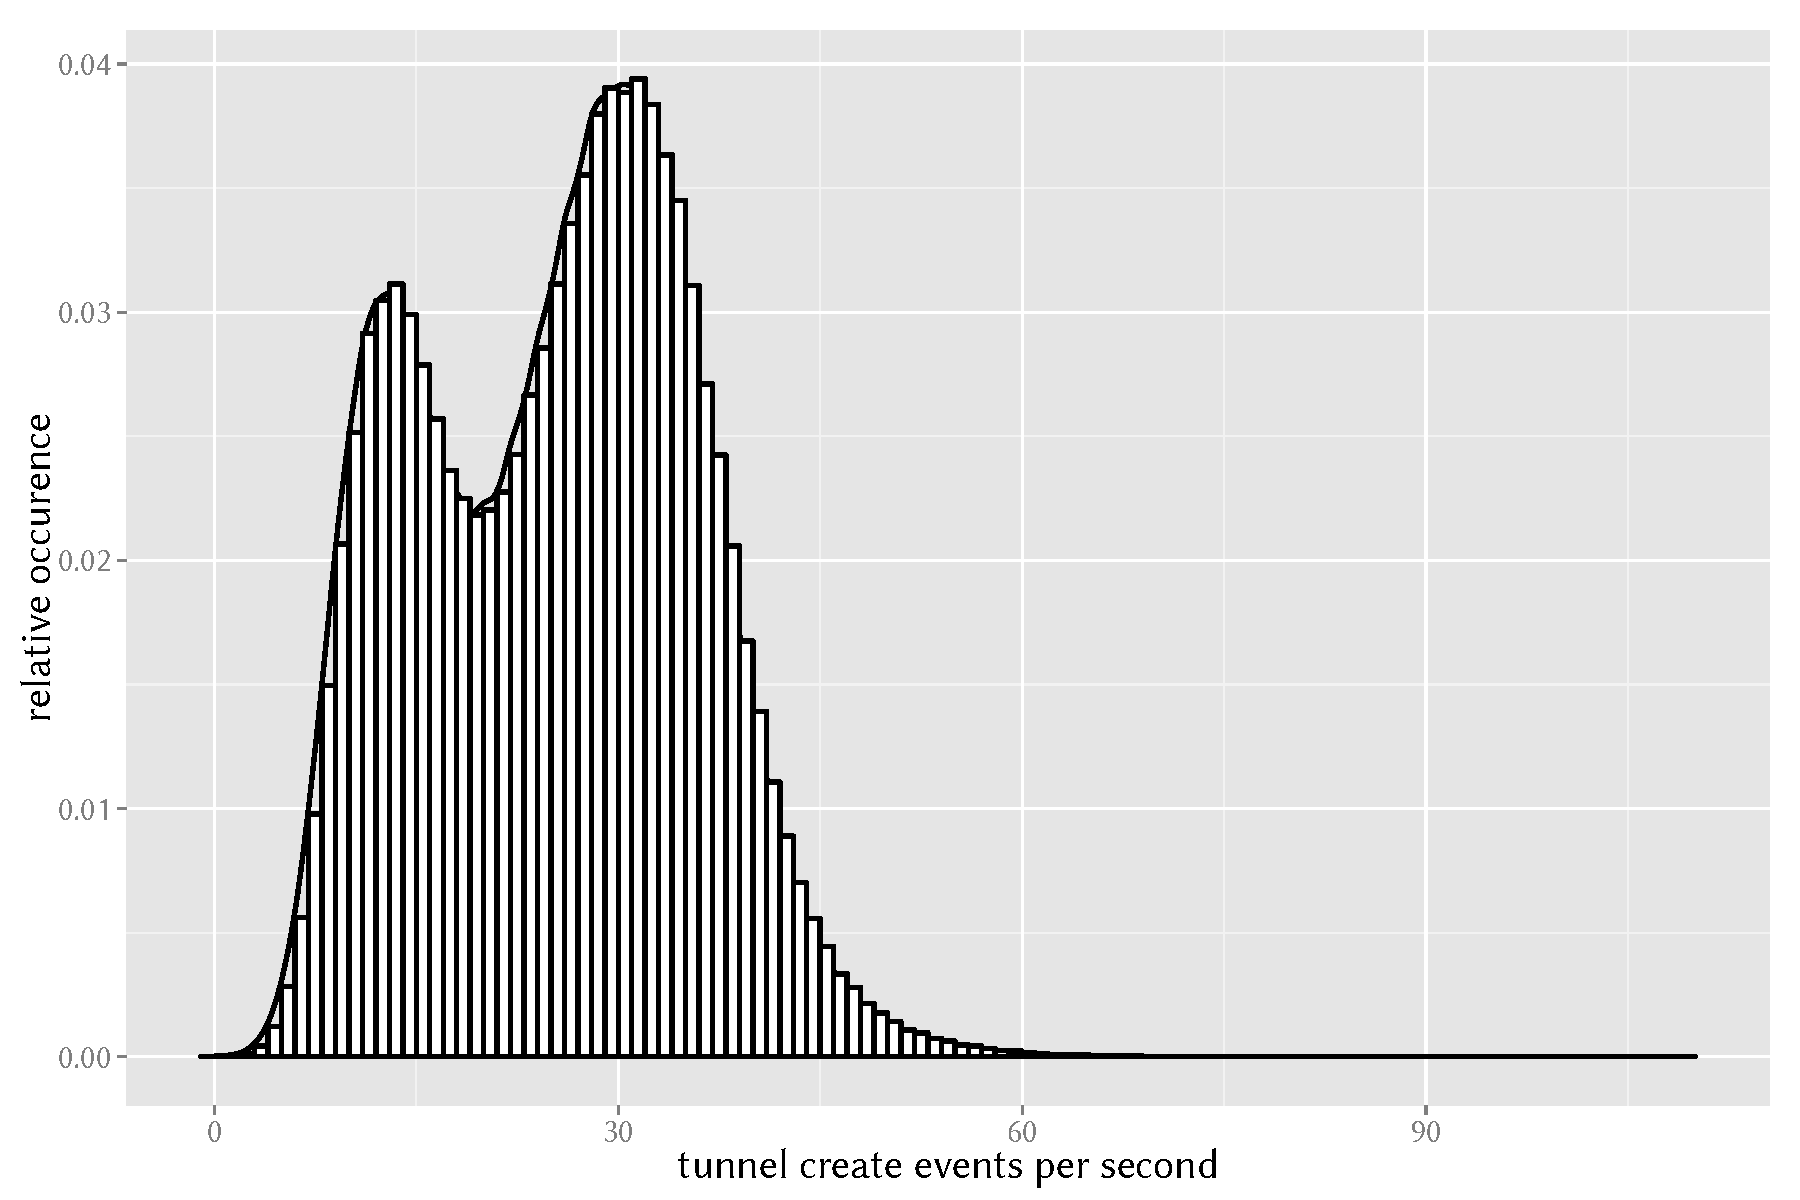
\includegraphics[width=0.9\textwidth]{images/R-create-frequency.pdf}
	\caption{Tunnel arrivals histogram overlaid with a density plot.}
\label{c4:fig:freq-arrivals}
\end{figure}

Figure~\ref{c4:fig:freq-arrivals} depicts a histogram the number of tunnel arrivals per second during the whole trace duration period. Of note is the clear bimodal nature with one peak around twelve and the other in the low thirties. While the distribution is rather compact around these two peaks, there are some clear outliers peaking at $107$ arrivals per second. If the hypothesis of the correlation between signaling load and number of arrivals holds, it can be assumed that load is not constant but rather switches between two modes with some periods of very high load induced by an increased number of arrivals.

\begin{figure}[htb]
	\centering
	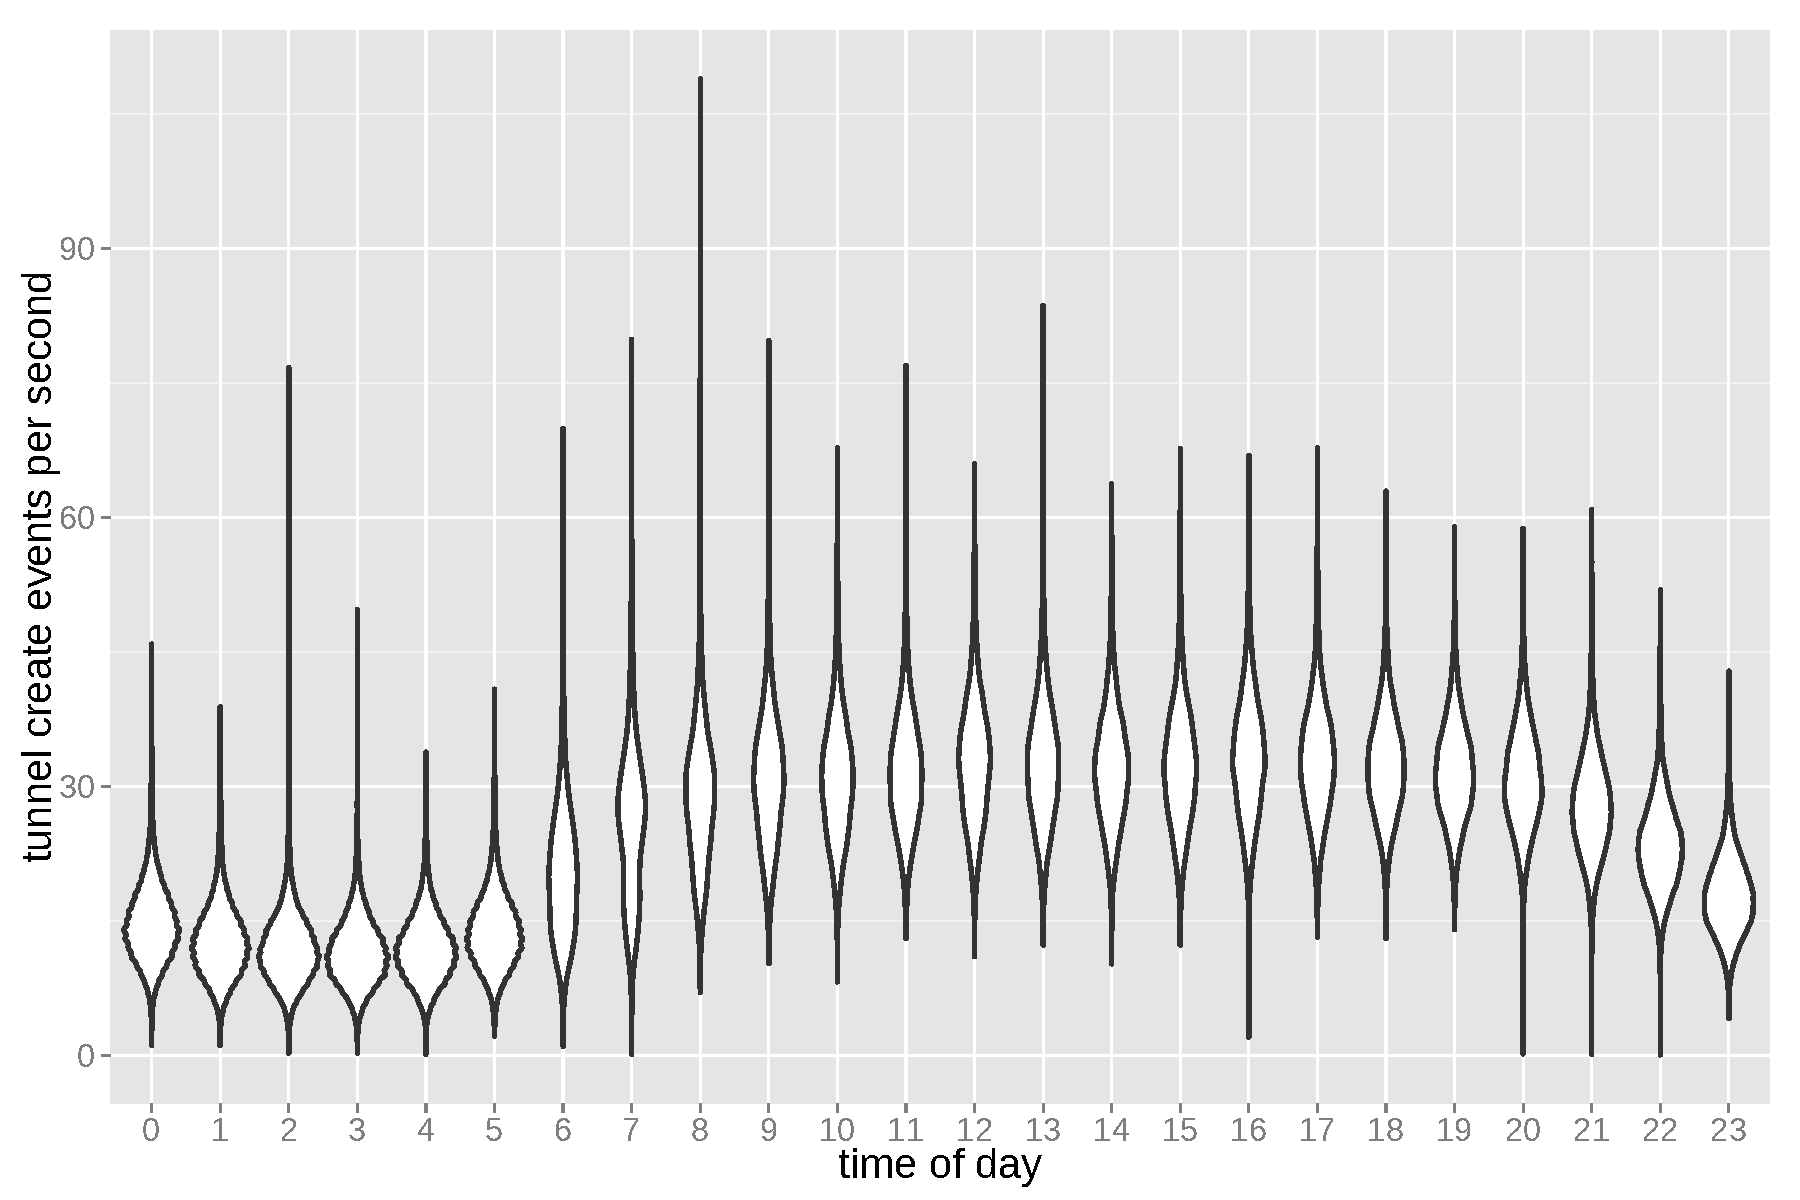
\includegraphics[width=0.9\textwidth]{images/R-createspersecond-1h-violin.pdf}
	\caption{Violin plot of tunnel arrivals in one second per time of day.}
\label{c4:fig:freq-arrivals-per-second-violin}
\end{figure}

A reasonable cause for the occurrence of these two modes can be found in the diurnal arrival patterns. Figure~\ref{c4:fig:freq-arrivals-per-second-violin} contains a violin plot of the tunnel arrivals. This type of plot is similar to a box plot but additionally shows the density of the individual items on the vertical axis. Here the arrivals are broken down to hourly slots. 

The nocturnal plateau of arrivals between midnight and \formattime{5}{0}{0} and the longer daytime plateau between \formattime{8}{0}{0} and \formattime{19}{0}{0} match the two modes found in the histogram. In between are short transition phases. The density of the arrivals during daytime indicates a spread of the number of arrivals over a larger range. This could be an indication of load fluctuations in the system.

\begin{figure}[htb]
	\centering
	\begin{subfigure}[b]{0.5\textwidth}    
		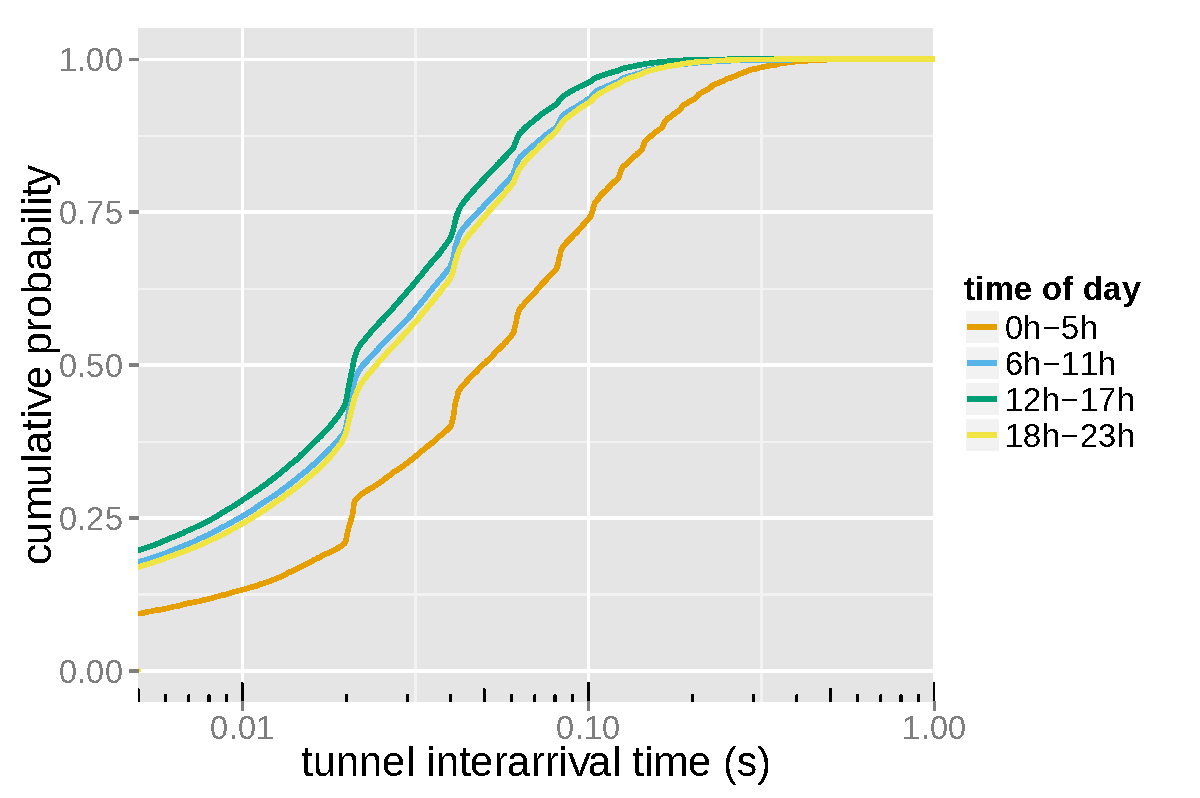
\includegraphics[width=\textwidth]{images/R-IAT-successful-2h-ecdfs.pdf}
		\caption{All tunnel requests.}
		\label{c4:fig:IAT-ecdf-2h-successful}
	\end{subfigure}%
	~
		\begin{subfigure}[b]{0.5\textwidth}
		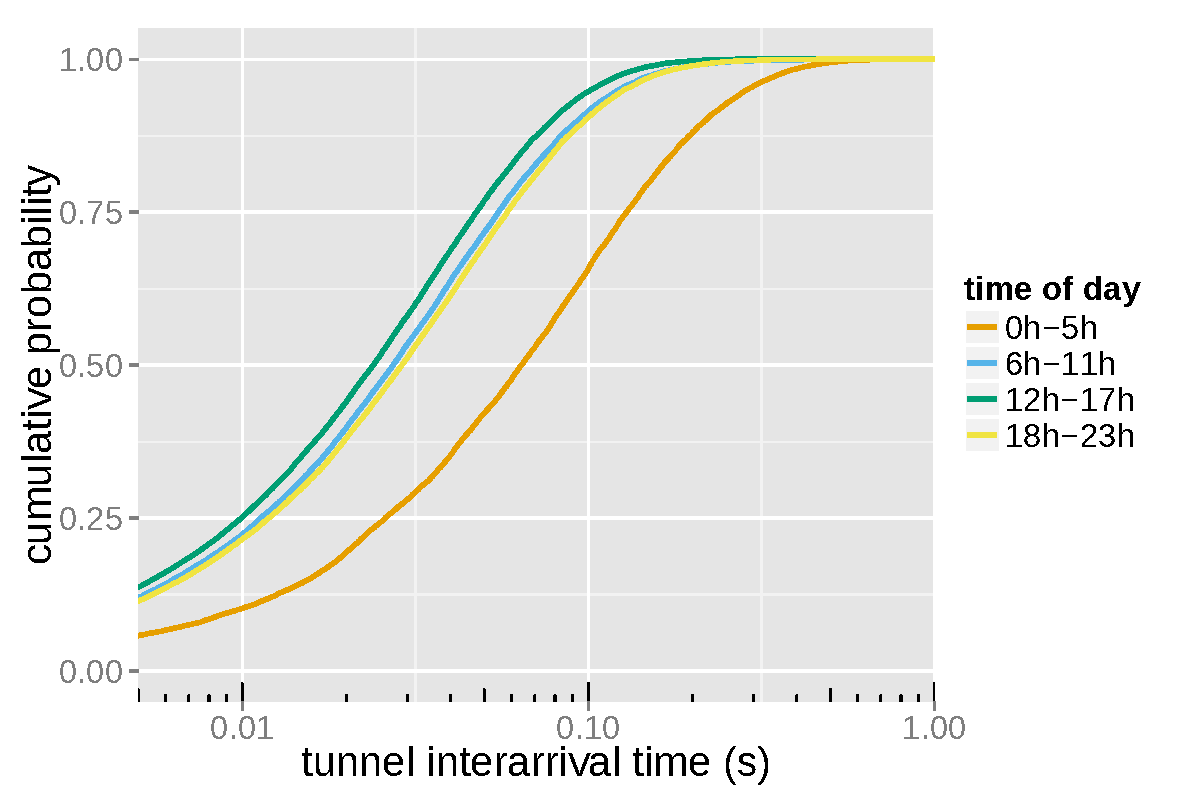
\includegraphics[width=\textwidth]{images/R-IAT-fromflows-ecdfs-2h.pdf}
		\caption{Only tunnels with data flows.}
		\label{c4:fig:IAT-ecdf-2h-active}
	\end{subfigure}

	\begin{subfigure}[b]{0.5\textwidth}
		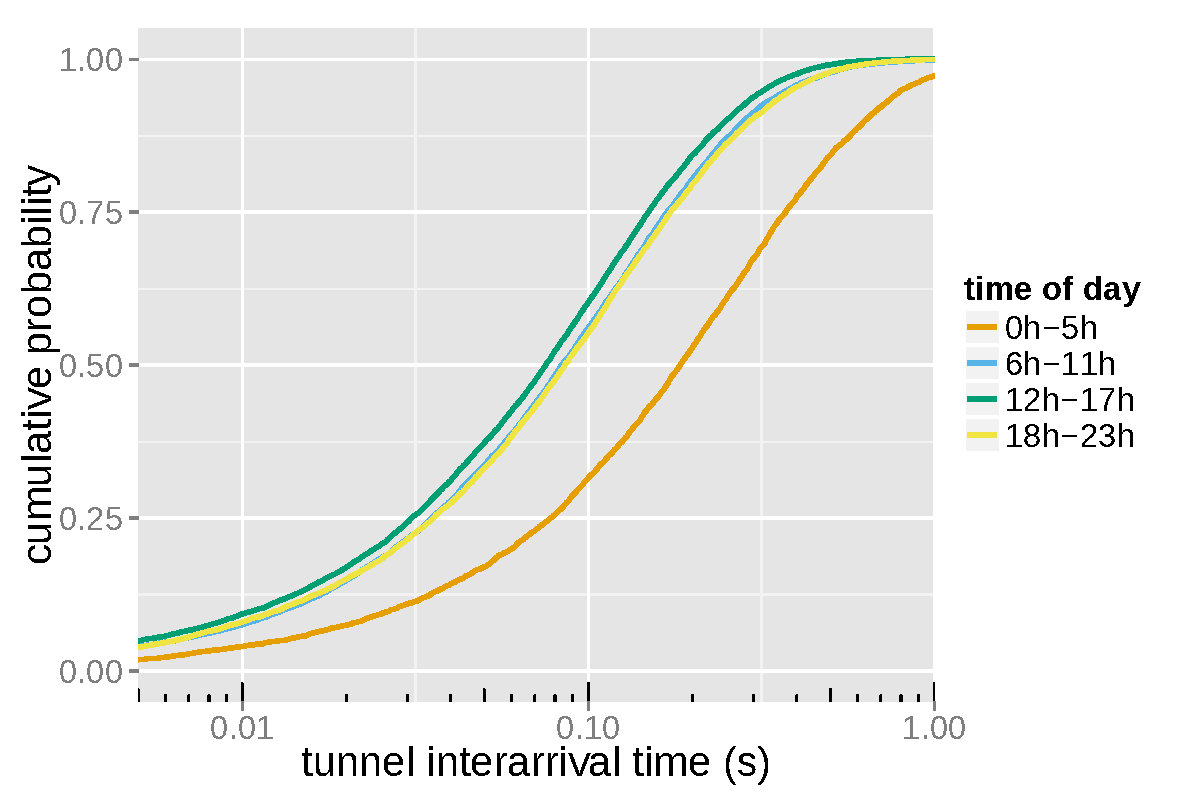
\includegraphics[width=\textwidth]{images/R-IAT-fromflows-gprs-ecdfs-2h.pdf}
		\caption{Tunnels with data flows initiated in \gls{GPRS}.}
		\label{c4:fig:IAT-ecdf-2h-active-gprs}
	\end{subfigure}%
	~
	\begin{subfigure}[b]{0.5\textwidth}
		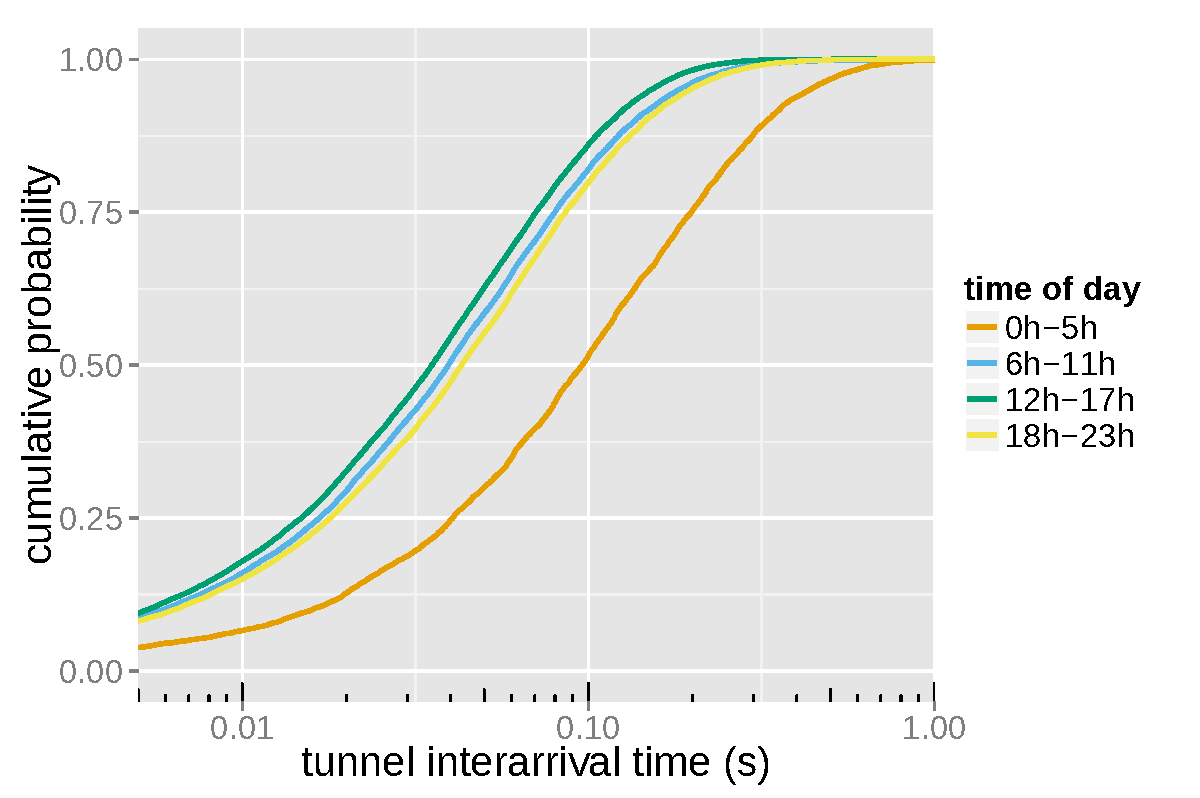
\includegraphics[width=\textwidth]{images/R-IAT-fromflows-umts-ecdfs-2h.pdf}
		\caption{Tunnels with data flows initiated in \gls{UMTS}.}
		\label{c4:fig:IAT-ecdf-2h-active-umts}
	\end{subfigure}
	\caption{\acrshortpl{ECDF} of the tunnel \acrshort{IAT} in seconds by time of day.}
\label{c4:fig:IAT-ecdf-2h}
\end{figure}

Complementing the arrival rate evaluation is the investigation of the tunnel \gls{IAT}. This metric is more sensitive to short time fluctuations of arrivals and more suited to describe the arrival process for use in the proposed load model.

The overall picture of all arrivals is given in the \gls{ECDF} of Figure~\ref{c4:fig:IAT-ecdf-2h-successful}, again broken down by time of day. Obviously the the same previously observed diurnal load oscillation can again be perceived. The median \glspl{IAT} fall in the range of \SI{20}{\milli\second} and \SI{60}{\milli\second}, enveloped by the \formattime{16}{0}{0} and \formattime{2}{0}{0}distributions on with the lowest and highest \gls{IAT} respectively. Additionally, tunnel arrivals are occurring at an increased frequency with an interval of multiples of \SI{20}{\milli\second}, which generates these wave-like steps in the \gls{ECDF} plot. As this is happening very regularly at every time of the day, a source inside the mobile network is indicated.

A hypothesis as to the origin of this effect is the value of the \gls{TTI}. This property determines the duration of a mobile network's radio transmission slot. In \gls{3GPP} standards up to \gls{UMTS} the default value of the \gls{TTI} is either \SI{10}{\milli\second} or \SI{20}{\milli\second}, newer versions of the specification set the value to \SI{2}{\milli\second} (in \gls{HSPA}) or even \SI{1}{\milli\second} (for \gls{LTE}). The absolute time of every transmission slot is also synchronized across every base station in the whole mobile network, which makes the \gls{TTI} noticeable even when not measuring directly at the radio link. 

The observed step-width of \SI{20}{\milli\second} therefore indicates that the tunnel establishment signaling procedure includes at least one trip from the mobile device over the radio interface. This makes sense, as the tunnel is typically created during the \gls{GPRS} Attach procedure, which is indeed initiated at the user's device. Unfortunately, this gives the arrival process batch properties. As a result the load at the \gls{GGSN} increases momentarily when a batch arrives. The \gls{GGSN} would then need to process more requests simultaneously than if the arrivals followed a smooth stochastic distribution.

This effect becomes more peculiar when the tunnel arrivals are further broken down. Figure~\ref{c4:fig:IAT-ecdf-2h-active} only displays arrivals of tunnels that actually transported user traffic during their lifetime. Here, the influence of the effect is visually unnoticeable. This could be attributed to the fact that most active data connections during the time of the trace recording were already using almost exclusively \gls{HSPA} or better, which sees the much lower \gls{TTI}. Only older, regular phones establish plain \gls{UMTS} connections and often do not even use it.

The discrimination of the \gls{IAT} distribution by \gls{RAT} that was used during the creation of the tunnel reveals no further information. Due to the much lower number of connections the \gls{GPRS} distributions are shifted to much higher intervals than the \gls{UMTS} specific distributions.


%%%%%%%%%%%%%%%%%%%%%%%%%%%%%%%%%%%%%%%%%%%%%%%%%%%%%%%%%%%%%%%%%%%%%%%%%%%%%%%
\subsection{\texorpdfstring{\acrshort{gtp}}{GTP} Tunnel Message Processing Time}

Finally, the \gls{GGSN}'s processing time of \gls{gtp} tunnel management messages is investigated. Potentially, this can be a direct measure of the load at the node. In times of higher load one would expect a higher processing time of signaling messages.

From the network trace the processing time can be calculated by two timestamps in each record.
As the trace is recorded at the Gn interface these timestamps represent the points in time the \gls{gtp} signaling request and subsequent response pass on the link to and from the the \gls{GGSN}. Therefore, they can also be interpreted as the start and finish of the involved processing at the \gls{GGSN}.

Generally, the processing time of all three message types --- i.e., creates, deletes and updates --- could be calculated. It would be of special interest to know if the setup time of tunnels is influenced by anything, as this is one of the \gls{GGSN}'s most time-sensitive jobs and can impact the time a user has to wait before being able to actually transfer data. Unfortunately, due to unrecoverable issues with the recording of the dataset, the timestamps for both the create and delete messages records were completely unreliable and did not allow for an investigation of the processing time. 

Only \gls{gtp} update messages were unaffected and gave the opportunity for further investigation. The trace contains roughly two orders of magnitude more update messages than either creates or deletes, spread out almost evenly over the whole observation period. Therefore, a node load investigation should still be possible with just the updates messages.

\begin{figure}[htb]
	\centering
	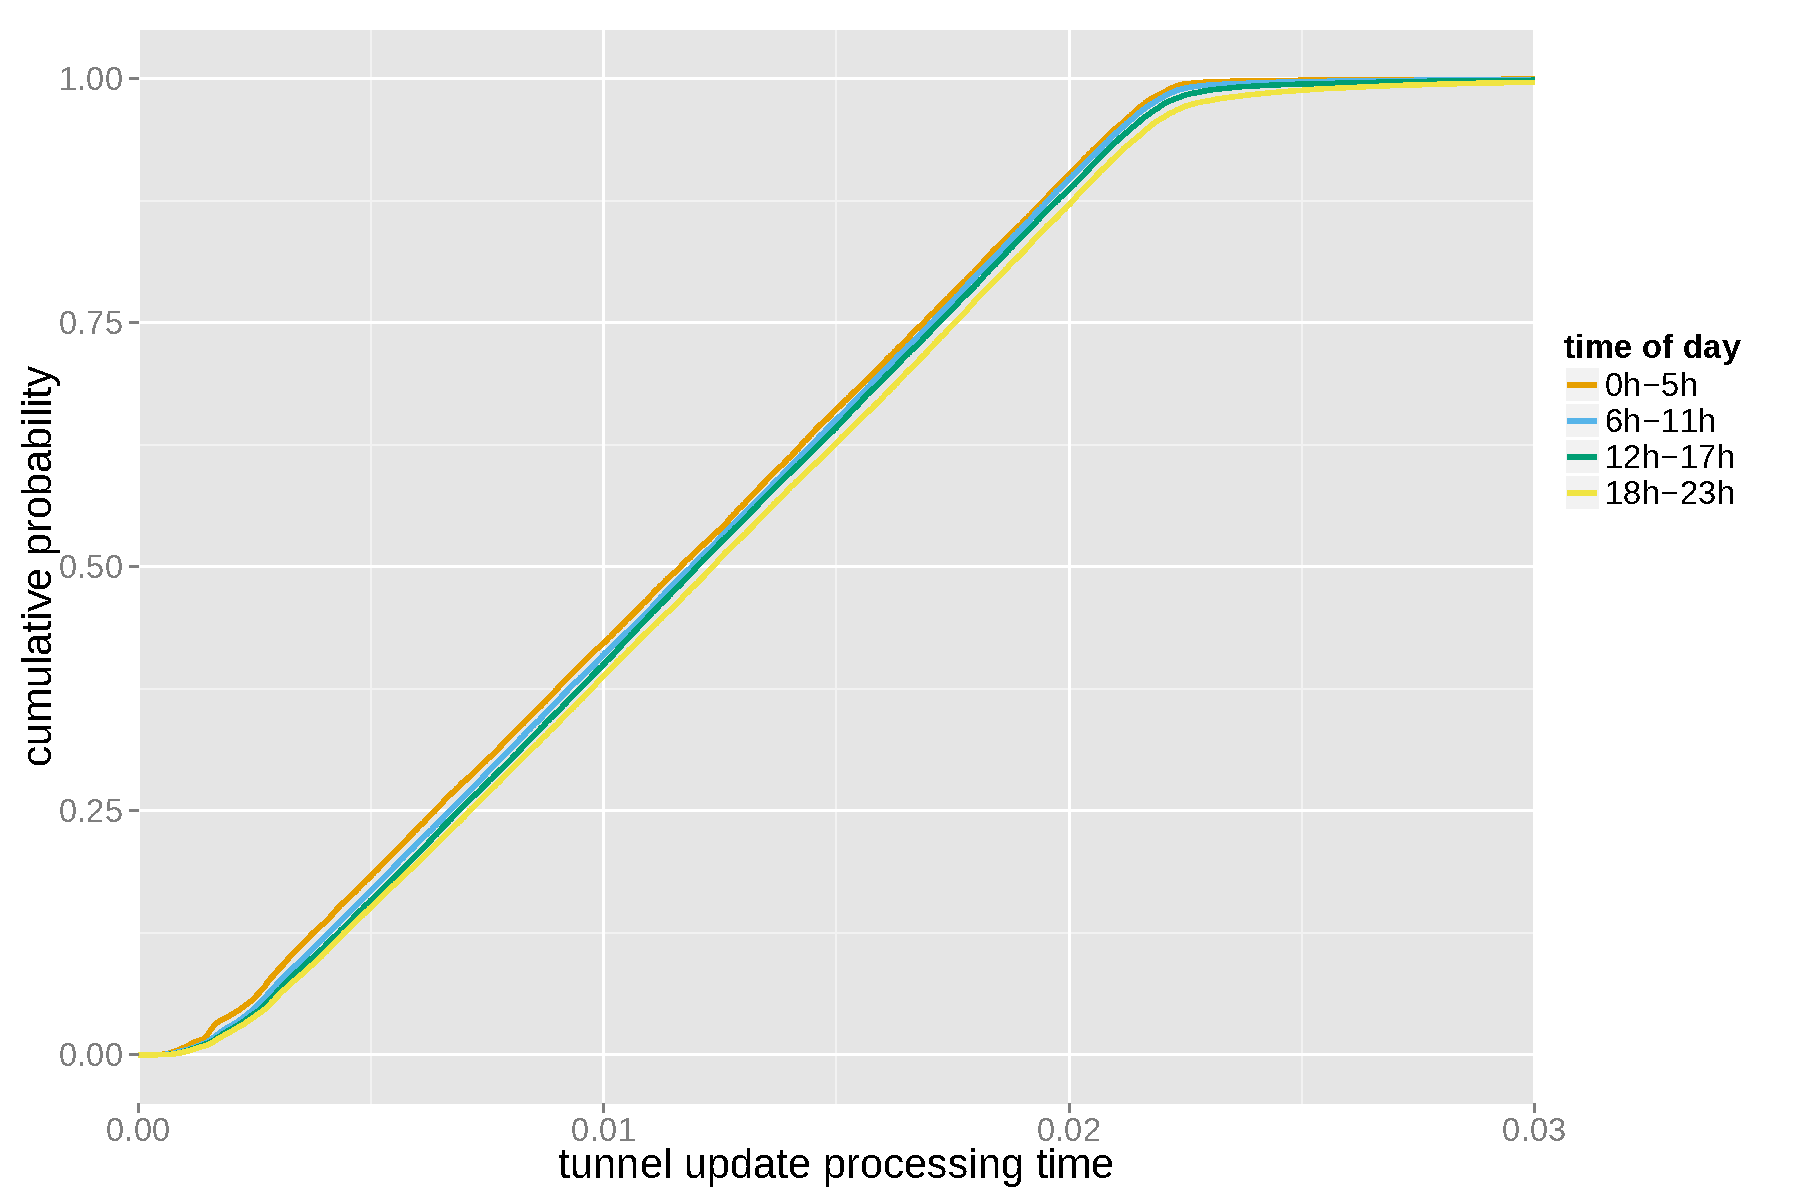
\includegraphics[width=0.9\textwidth]{images/R-update-time-cdfs.pdf}
	\caption{\acrshortpl{ECDF} of the time in seconds it takes a \acrshort{GGSN} to process a \acrshort{gtp} update event, separately plotted for four time slots each day.}
	\label{c4:fig:update-time}
\end{figure}

Figure~\ref{c4:fig:update-time} depicts a band of \glspl{ECDF} for the processing time of update messages by time of day. The processing time distribution almost perfectly follows a continuous uniform distribution between \SI{2}{\milli\second} and \SI{22}{\milli\second}. Only the upper end displays a slight long-tail behavior. The impact of the time of day is very slim with slightly higher processing times during the evening, the same time frame which also experienced an elevated arrival rate.

The occurrence of a continuous uniform distribution is rather unexpected as these do not usually occur in computing processes. According to the central limit theorem one would rather expect to see a normal distribution influenced by, e.g., process scheduling or other queuing artifacts. The source of this effect is still unknown and the current dataset does not allow for a more thorough investigation. Still, the fact that a higher update processing time coincides with an increase in the arrival rate points to an influence of tunnel messaging on the load of a \gls{GGSN}.



%%%%%%%%%%%%%%%%%%%%%%%%%%%%%%%%%%%%%%%%%%%%%%%%%%%%%%%%%%%%%%%%%%%%%%%%%%%%%%%
\subsection{Statistical Evaluation and Data Fitting}
\label{c4:sec:statistical_evaluation}

The uncovered empirical distributions for both the tunnel duration and the tunnel \gls{IAT} are now to be matched against theoretical probability distributions. Therefore, a univariate distribution fit to the experimental data was conducted. Having a concise representation for the empirical data will help in creating a model of the core network, which is the task conducted in the sections following after this.


%%
\paragraph{\gls{IAT} Fitting}

\begin{figure}[htb]
	\centering
	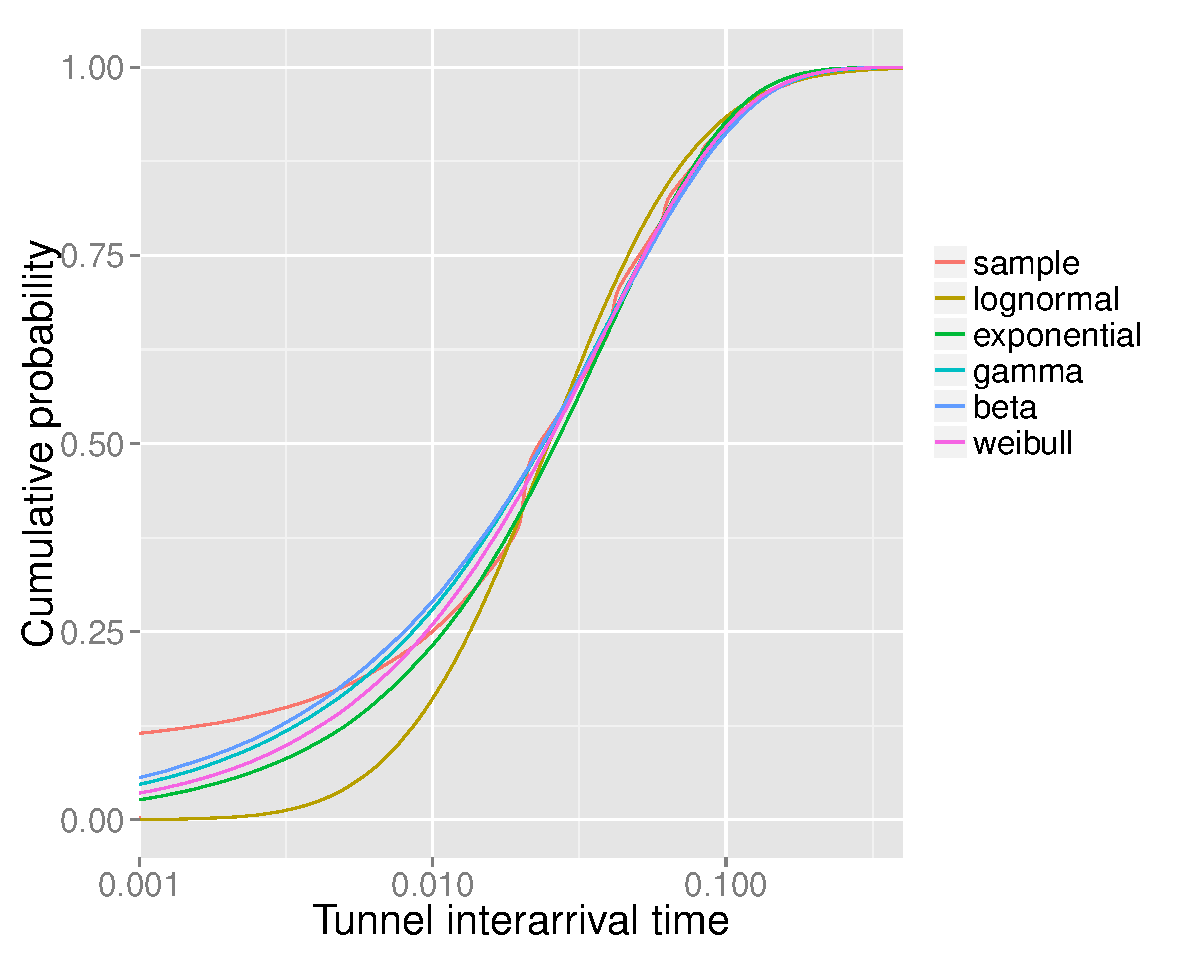
\includegraphics[width=0.9\textwidth]{images/R-IAT-ecdfs.pdf}
	\caption{Sampled inter-arrival time \acrshort{CDF} and fitted theoretical distributions.}
\label{c4:fig:IAT-cdfs}
\end{figure}

In order to investigate the tunnel \gls{IAT}, Figure~\ref{c4:fig:IAT-cdfs} displays the overall \gls{ECDF} with fits for various basic probability distributions. Each of the fits was generated through the method of moments matching.

The goodness of these fits was checked both visually using the \glspl{CDF} plots and numerically with goodness of fit measures, using Pearson's correlation coefficient and Pearson's $\chi^2$ test. Unfortunately, none of the probability distributions reaches the significance level for $\chi^2$. This can probably be largely attributed to the various previously described artifacts in the data. Matching them visually, the exponential fit seems to be reasonably close to the experimental data.

\begin{figure}[htb]
	\centering
	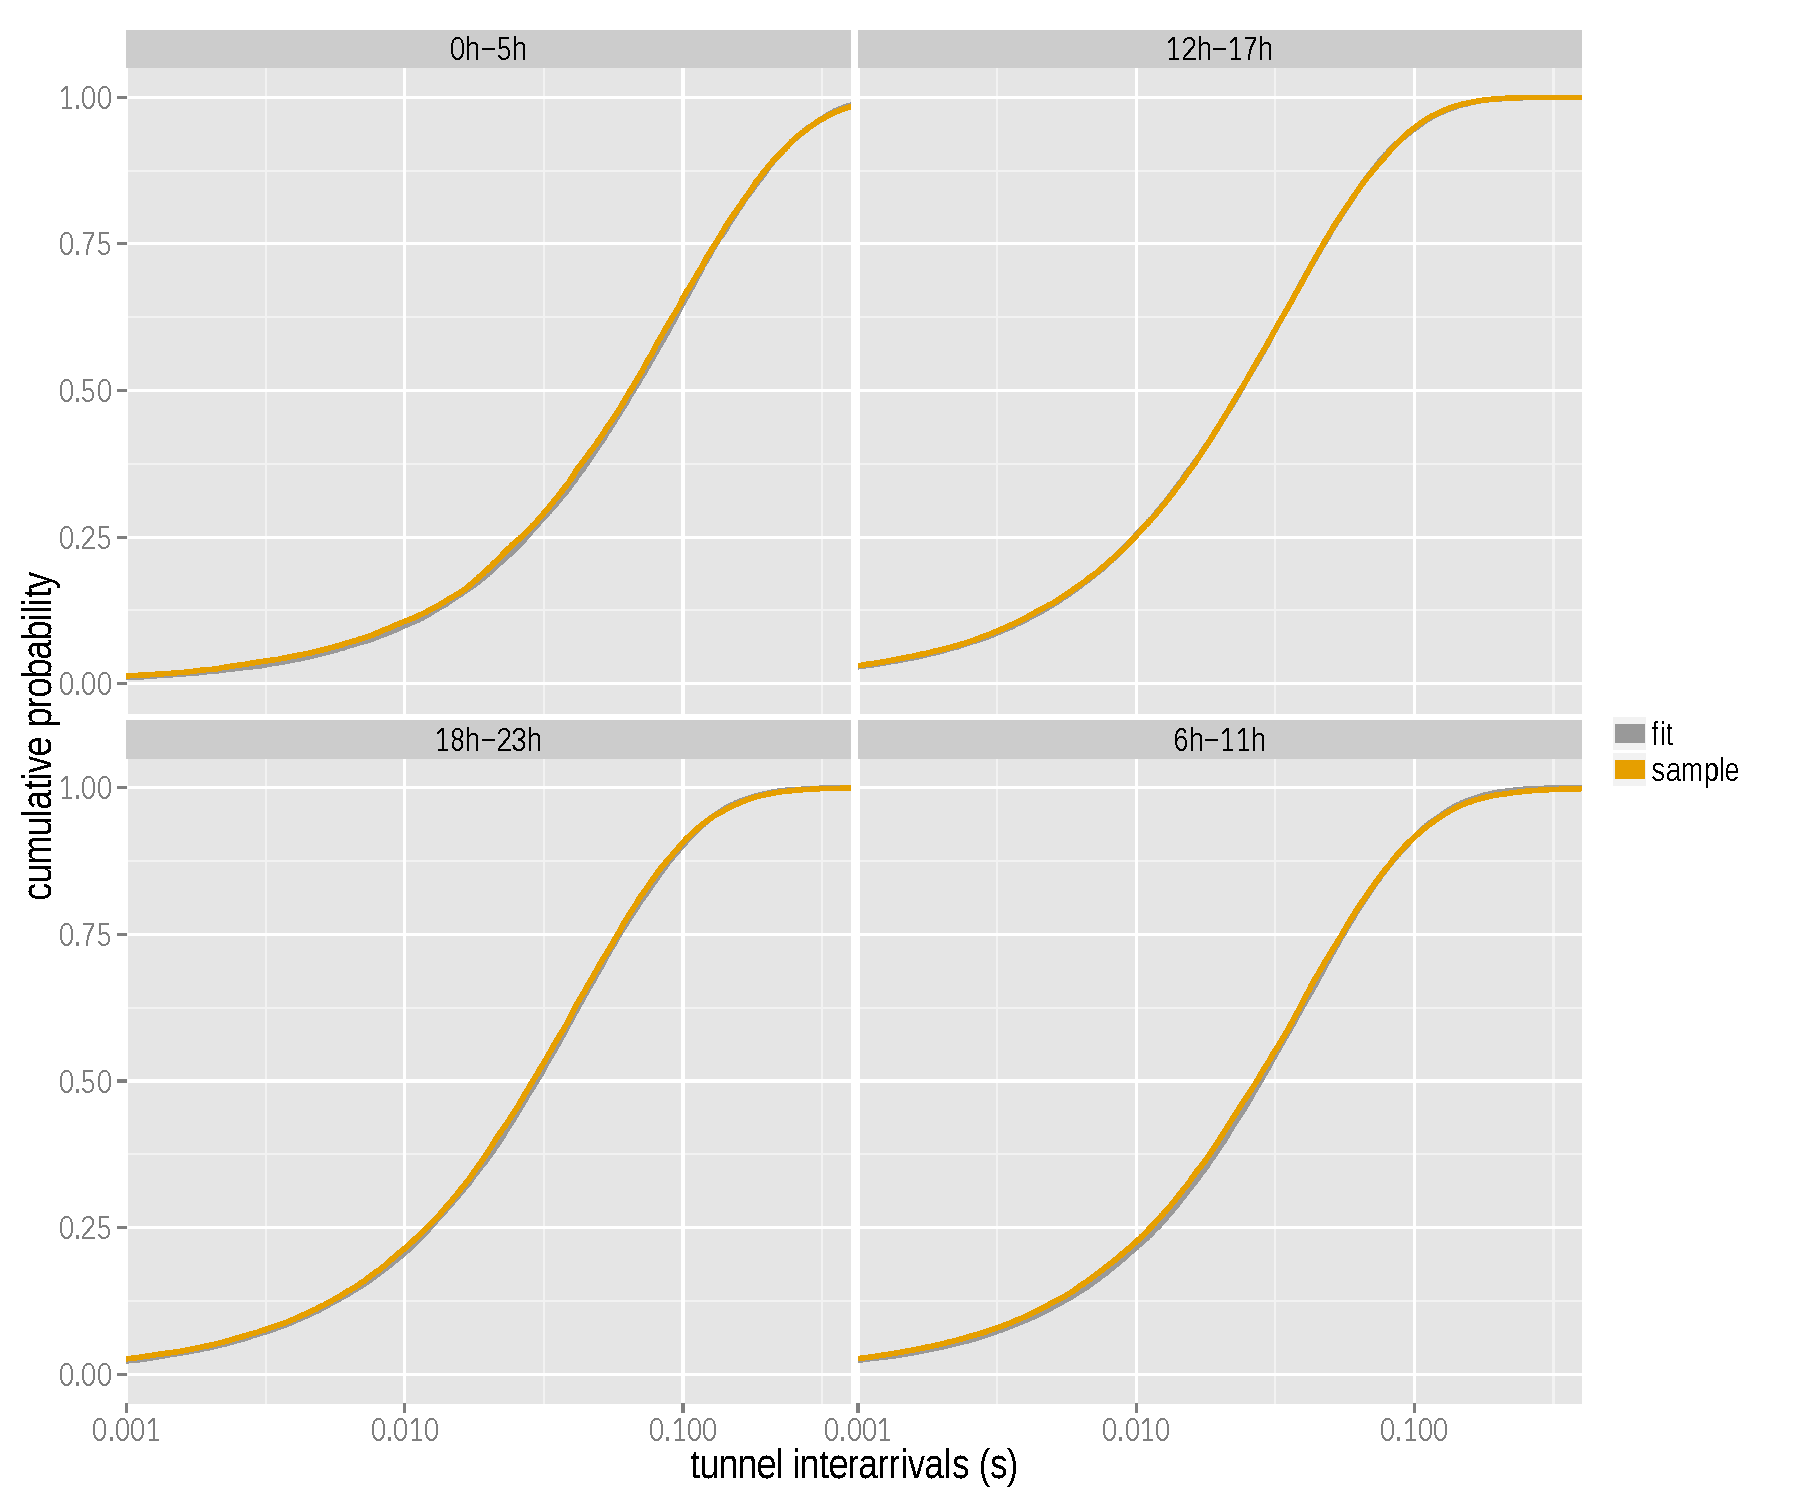
\includegraphics[width=0.9\textwidth]{images/R-IAT-active-fit-cdf-facets.pdf}
	\caption{Empirical and exponentially fitted \acrshortpl{CDF} of the tunnel \acrshort{IAT} by time of day. \acrshortpl{CDF} are overlapping as the coefficient of determination is close to $1$.}
\label{c4:fig:pdparrivalsecdf}
\end{figure}

To improve the fits, two modifications were made to the process. First, to remove the \SI{20}{\milli\second} steps, only the active tunnels were taken into consideration. Second, the overall \gls{IAT} distribution was once again split up into time of day slots. The overall distribution is just a superimposition of the individual slots anyway. Therefore, this should further improve the fidelity of the fits.

\begin{table}[htb]
\caption{Parameters for the exponentially distributed inter-arrival times and corresponding Pearson correlation coefficients.}
\label{c4:tab:IAT-fits}
	\centering
	\begin{tabu}{X[0.9,l]X[r]X[r]} 
	\toprule
	\textbf{Time of Day} & $\mathbf{\lambda}$ & $\mathbf{R_{arrival}}$\\ 
	\midrule
	0h-5h   & $10.67477$ & $0.995$ \\
	6h-11h  & $24.53298$ & $0.992$ \\
	12h-17h & $29.2504$  & $0.993$ \\
	18h-23h & $23.49983$ & $0.986$ \\
	\bottomrule
	\end{tabu}
\end{table}

The results are depicted in Figure~\ref{c4:fig:pdparrivalsecdf}. To improve plot visibility only four larger time slots are displayed here while the actual fits were conducted for each hour slot. Parameters for the exponential distribution $F(x) = 1- e^{-\lambda x}, x \geq 0$ and the corresponding correlation coefficients to the original data for the four time slots are given in Table~\ref{c4:tab:IAT-fits}. The fitted functions match the empirical data quite well, with some deviation present at the left tail but an overall positive correlation coefficient approaching $1$.


%%
\paragraph{Duration Fitting}

The second fitting effort surrounds the empirical data concerning the tunnel durations. However, none of the basic probability distributions (including exponential, gamma, and Weibull distributions) fit the tunnel duration even remotely. One of the reasons for this is probably that the tunnel duration is influenced by an overwhelming amount of factors, which were previously described. This superposition, especially with the user behavior, will result in unpredictable results that does not follow any basic probability distribution.

\begin{figure}[htb]
	\centering
	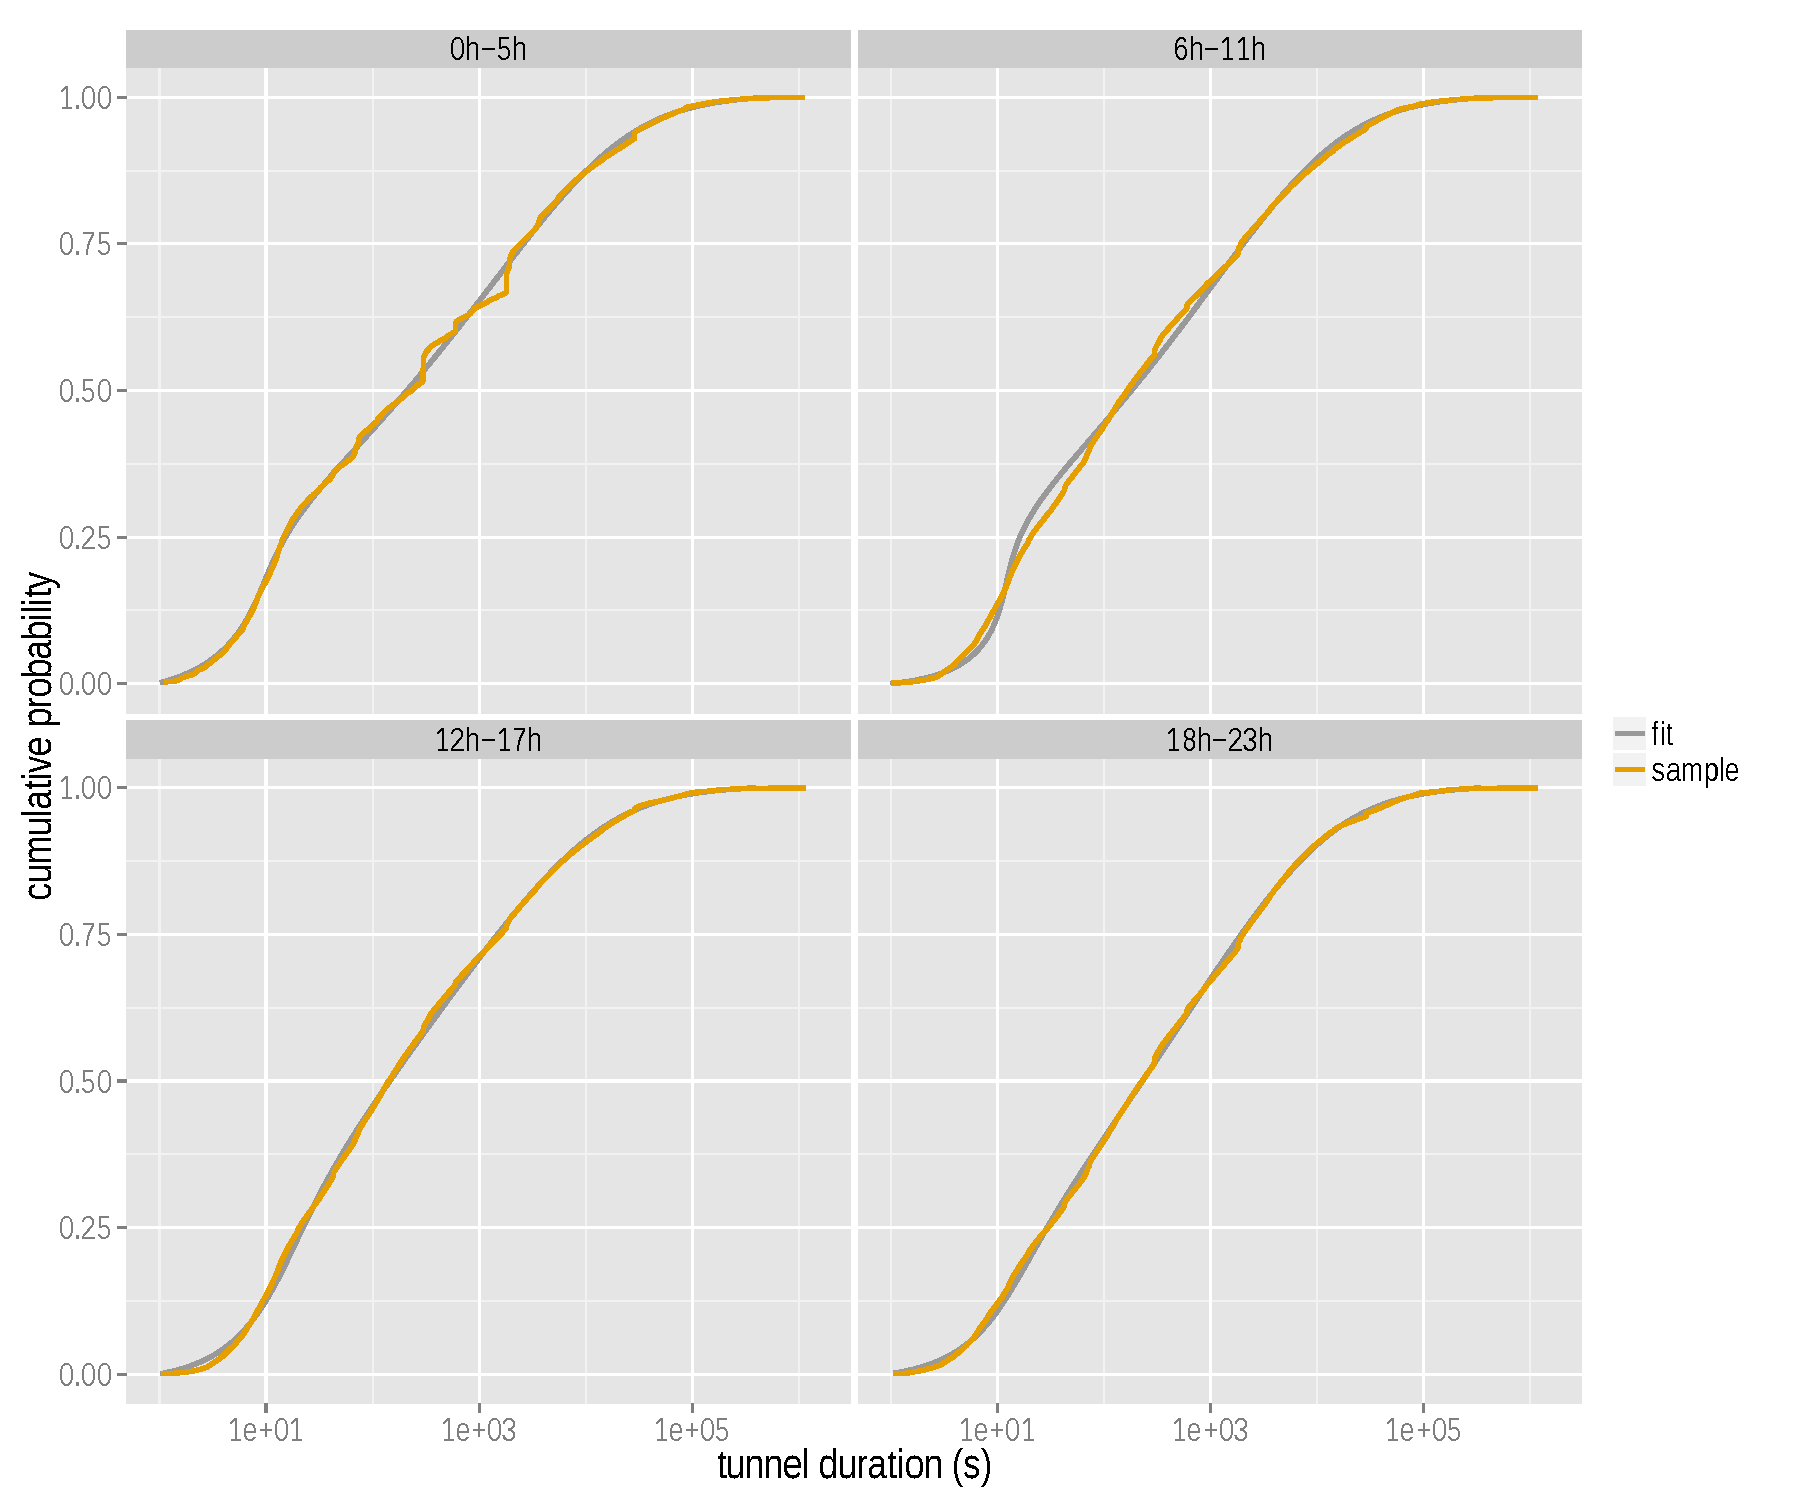
\includegraphics[width=0.9\textwidth]{images/R-duration-fit-cdf-facets.pdf}
	\caption{Empirical and fitted \acrshortpl{CDF} of the tunnel duration by time of day with fitted rational functions.}
\label{c4:fig:fittedsdurationlots}
\end{figure}

Instead, rational functions are fitted to the \glspl{ECDF} using the proprietary third-party tool \textit{Eureqa}~\cite{eureqa_paper, eureqa_software}. This allows for a much closer fit as seen in Figure~\ref{c4:fig:fittedsdurationlots}, but limits its application in the statistical evaluation.

\begin{table}[htb]
\caption{Inverse rational functions fitted to the \acrshortpl{ECDF} of the tunnel duration by time of day and correlation coefficients of the fit.}
\label{c4:tab:fits-duration}
	\centering
	\begin{tabu}{X[1.1,l]X[4.5,r]X[r]} 
	\toprule
	\textbf{Time of Day} & \textbf{Inverse Serving Time \gls{CDF} Representation} & $\mathbf{R_{dur}}$\\ 
	\midrule
	0h-5h & $0.919 - 60.614y - 3498.78y^3 - \frac{110.707y + 2289.94y^3}{y - 1.005}$ &  $0.999$ \\
	6h-11h & $1 + 117.484y - 368.643y^2 - \frac{1720.13y^4}{y - 1.004}$ & $0.999$ \\
	12h-17h & $0.953 + 69.491y + \frac{81146.1y^3 + 1.086\times10^6y^5}{805 - 802.01y}$ & $0.999$ \\
	18h-23h & $0.912 + 82.056y - \frac{2936.93y^4}{1.945y - 1.953}$ & $0.999$ \\
	\bottomrule
	\end{tabu}
\end{table}

	% high precision:
	% 0h-5h & $0.919208 - 60.6136y - 3498.78y^3 - \frac{110.707y + 2289.94y^3}{y - 1.00469}$ &  $0.999$ \\
	% 6h-11h & $1 + 117.484y - 368.643y^2 - \frac{1720.13y^4}{y - 1.0041}$ & $0.999$ \\
	% 12h-17h & $0.952566 + 69.4907y + \frac{81146.1y^3 + 1.08572\times10^6y^5}{805 - 802.01y}$ & $0.999$ \\
	% 18h-23h & $0.911924 + 82.0562y - \frac{2936.93y^4}{1.94468y - 1.9532}$ & $0.999$ \\

Table~\ref{c4:tab:fits-duration} contains the functions which were fitted to the \textit{inverse} \gls{CDF}. The inverse was chosen here to simplify the modeling and simulation process coming afterwards. The functions can be easily inverted again for other purposes. Both the \glspl{CDF} in the plot as well as the Pearson correlation coefficient, which again approach $1$, confirm the goodness of the fitted functions.


% \begin{table}
% \centering
% \caption{TAC Statistics}
% \begin{tabu}{|X|X|X[1.5]|X|X|X|} \hline
% & \textbf{\# of Flows} & \textbf{Total Traffic (Bytes)} &  \textbf{\# of Tunnels} & \textbf{\# of GTP Signalling Msgs} & \textbf{\# of Distinct IMSIs}\\ \hline
% Total          & 2234659247 & 122758578593993 (112TB)    & 16632094 & 409733865 & 1255293 (all) / 1030895 (with flows) \\ \hline
% In TAC DB      & 2228315260 & 122716712007150 (111.61TB) & 14565430 & 372662108 & 1015891 \\ \hline
% Smartphones    & 459990512  & 15721818747754 (14.30TB)   & 10030734 & 311342846 & 476675  \\ \hline
% Regular phones & 5705832    & 448140315058 (0.41TB)      & 897529   & 3860162   & 116124  \\ \hline
% 3G dongles     & 1487230062 & 92215931895630 (83.87TB)   & 2114756  & 39053819  & 315003  \\ \hline
% Android        & 241973565  & 7953178401958 (7.2TB)      & 2383255  & 177537567 & 175919  \\ \hline
% iOS            & 161408903  & 5481693567152 (5TB)        & 3145384  & 83374590  & 99679   \\ \hline
% Symbian        & 22827418   & 1332996529271 (1.21TB)     & 3520242  & 18479002  & 162790  \\ \hline
% Blackberry OS  &            & 128074907884 (0.12TB)      &          &           &         \\ \hline
% \end{tabu}
% \end{table}


%Devices with GTP signaling but no user plane traffic: (\#distinct imsis gtp db)-(\#distinct imsis flow db):
% $255293-1030895=224398\text{ or }17.88\%$

%%%%%%%%%%%%%%%%%%%%%%%%%%%%%%%%%%%%%%%%%%%%%%%%%%%%%%%%%%%%%%%%%%%%%%%%%%%%%%%%
%\subsection{Correlations to User Traffic}
% TODO, incl. measurements



%%%
% Direct signaling traffic overhead in relation to user traffic and induced network load

% GTP Header: 12 Byte
% IE header and footer: 2 Byte
% Maximum minimum data size including all \glspl{IE}: 221 Byte + 12 Byte Header + 2*37 Extension Header = 307 Byte
% Minimum size of message with just mandatory \glspl{IE}: 12 + 30 + 2*5 = 52 Byte

% 307 Bytes:
% calculation from our dataset
% Total maximum signaling traffic with this calculation: 117.15GB
% Ratio: 0.10\%
% 52 Bytes:
% Total maximum signaling traffic with this calculation: 19.84GB
% Ratio: 0.02\%
% Total traffic: 122758578593993


% signaling calc:
% gtp signaling traffic volume estimation $v_s$ = (1059B gtp message + 8B udp header + 20B ipv4 header) = 1087B * 409733865 number of request/response pairs * 2 (2 messages per pair) = 8,9076142E11B
% ratio to total $r=\frac{v_s}{v_t}=0.72\%$  $v_t=122758578593993B$


%%
%TODO: radio access type plots, if we have the data
% We do not.
%
%\begin{figure}
%\centering
%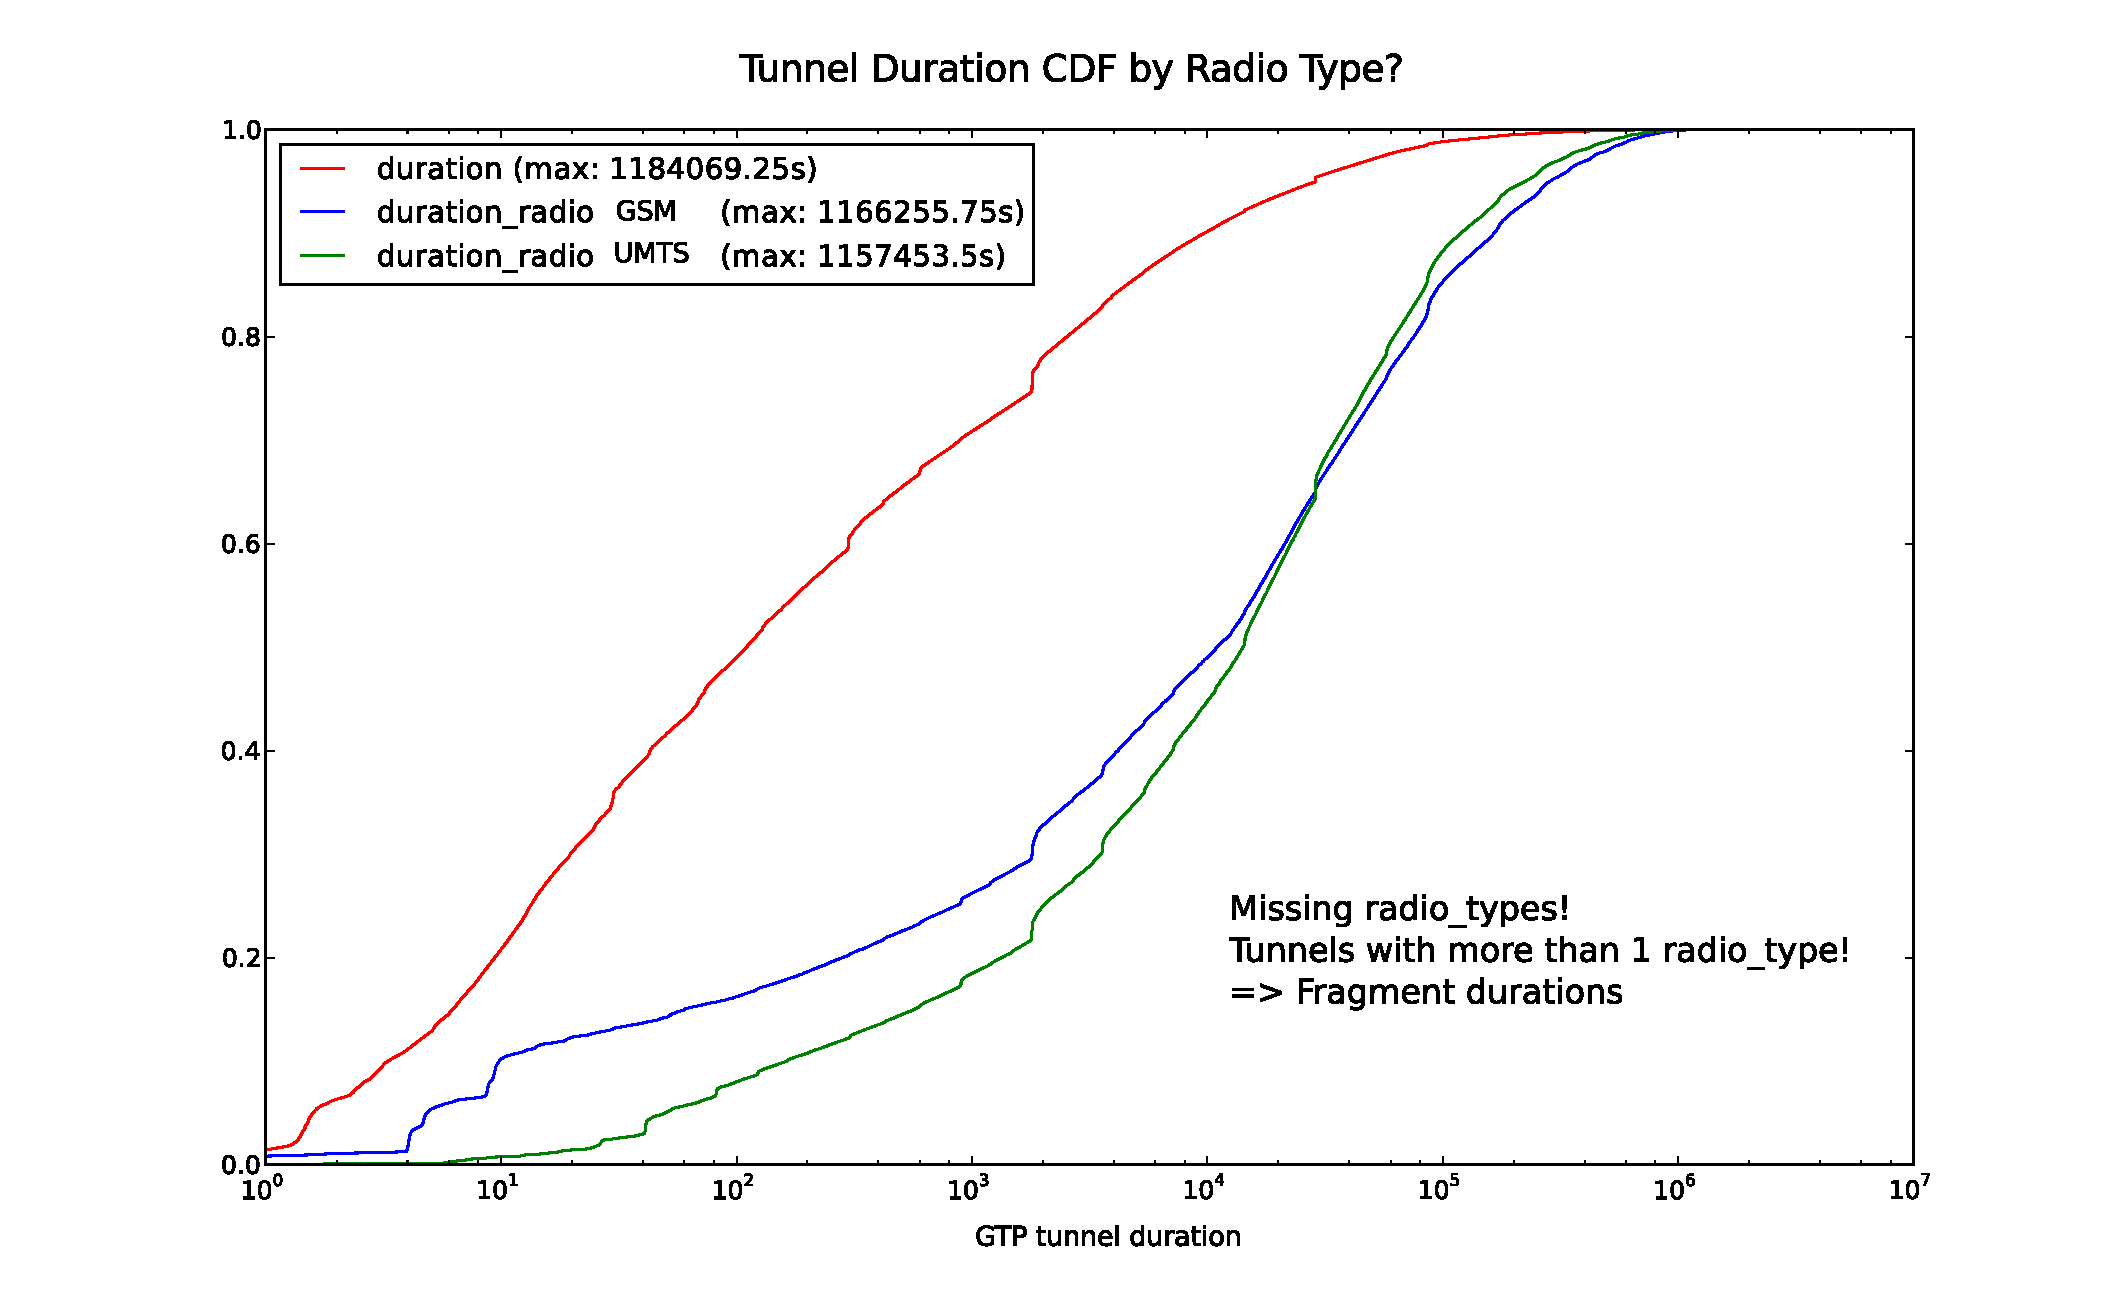
\includegraphics[width=\columnwidth]{figures/tunnel-dur-radio-cdf-mod.pdf}
%\caption{Tunnel duration distribution, separated for UMTS and GPRS radio access [NOTE: only in the last tunnel segment; and majority of radio types %is unknown anyway.}
%\label{fig:cdf-duration-radio}
%\end{figure}


%%%%%%%%%%%%%%%%%%%%%%%%%%%%%%%%%%%%%%%%%%%%%%%%%%%%%%%%%%%%%%%%%%%%%%%%%%%%%%%%
%!TEX root = ../../dissertation.tex
%%%%%%%%%%%%%%%%%%%%%%%%%%%%%%%%%%%%%%%%%%%%%%%%%%%%%%%%%%%%%%%%%%%%%%%%%%%%%%%%
\section{Streaming Modeling}
\label{c3:sec:modeling}

As stated, the goal of this chapter is to model the measuring process and reliable streaming. This section will introduce our reliable \gls{TCP}-based streaming model. It is intended for easily comparing different protocol variants against each other and measuring all variants in one testbed. 

But first, because any evaluation of a model requires metrics, we describe ones appropriate to the model and give a rationale.
 
%%%%%%%%%%%%%%%%%%%%%%%%%%%%%%%%%%%%%%%%%%%%%%%%%%%%%%%%%%%%%%%%%%%%%%%%%%%%%%%%
\subsection{Metrics for Reliable Transport Streaming}
\label{c3:metrics}

When measuring anything related to video or even just image quality, one has the choice between conducting a subjective or objective assessment. 

During a subjective test, human assessors evaluate and rate video quality in a controlled environment with the results usually being aggregated into an overall relative quality score \gls{MOS}. Through the human element, conducting a subjective assessment is very time and resource consuming but it also achieves the highest precision.

This is where, objective video quality assessments come into play. Modern objective models attempt to recreate the features of the humans' visual perception and psychophysics and are calibrated by subjective assessments. Most objective models operate on a full reference approach, they directly compare the original reference video to the resulting video after being encoding or transmitted.

Two of the simplest full reference image quality metrics, which can also be applied on video, are the \gls{MSE} and \gls{PSNR}, defined as:

\begin{equation}
    \begin{aligned}
    MSE = \frac{1}{N} \sum_{i=1}^{N}(x_i - y_i)^2\\
    \text{and } PSNR = 10 \log_{10} \frac{L^2}{MSE},
    \end{aligned}
\end{equation}

with $N$ as the number of pixels in a frame and individual pixels $x$ and $y$ from the reference and output frame respectively. $L$ denotes the maximum value of a pixel. For grayscale or when investigating each color channel separately, usually $L = \SI{8}{\bit} = 255$.  \cite{objective-vqa}

Image quality models can by nature only test for spatial distortions of a single image. This includes a general blockiness or blurriness, noise, or reduced resolution. Dedicated video quality assessments can additionally take temporal metrics into account, e.g. frame rate anomalies. Such models are being researched and standardized by the \gls{ITU} and \gls{VQEG} for example in \cite{ituJ144, ituJ246, ituJ247}.


When conducting dedicated streaming quality measurements, only this portion should be taken into account by a metric, and not the initial encoding process. During streaming only a specific subset of quality degradations can occur. Lost or late packets can cause missing blocks in a frame or frames to be skipped completely. Initial thoughts concerning \gls{IPTV} \gls{QoE} have been given in \cite{ituG1080} and the influence of packet delay variations on playout buffers is investigated in \cite{rfc3393}The \gls{MDI} \cite{rfc4445} is an attempt to capture this behavior and relate it to the network \gls{QoS}. Its metric relies on two properties, the \gls{DF}, as a measure of the network's latency and jitter, and the media loss rate. Of special interest to this investigation is the \gls{DF}, which is calculated based on a virtual buffer (VB) of received stream data as

\begin{equation}
    \begin{aligned}
        VB = r_{rcv} - r_{drain} \\
        DF_i = \frac{\max(VB) - \min(VB)}{r_{drain}}
    \end{aligned}
\end{equation}
 
Reliable streaming has even less possibilities to degrade a video stream. Packets can not be out of order and loss is concealed by \gls{TCP}, meaning that the transmitted and the played video are identical. The only thing that can still happen, is portions of the video arriving too late to be played out at their intended point in time.
A potential reliable streaming quality assessment metric needs to keep track of the following properties:

\begin{itemize}
    \item The initial delay, which is the time delta between the start of the transmission and the start of the video play.
    \item The number and lengths of interruptions or stalls during playback.
    \item For adaptive streaming, the characteristics of the quality levels the video was played in. This includes the number of switching events and the duration of each level.
\end{itemize}

A concise metric covering all properties has not been defined yet. The \gls{CI} was defined in \cite{1498486} and used to determine quality in \gls{P2P} live streaming. It is defined as \enquote{the number of segments that arrive before or on playback deadlines over the total number of segments} and with this partly captures the stalling property. In \cite{5634160} and \cite{DBLP:journals/corr/SeyedebrahimiBP13} a so-called \gls{PI} is defined and evaluated. The definition $I_p = uv$ is simply based on the number of stalls $u$ and the average stall duration $v$. 

Generally, most research operates just directly on these three properties, which allows for the most freedom in usage scenarios. The streaming measurement model presented in the following section also works with the assumption, that only the three properties are of importance. The model assumes no special metric, the individual properties can be directly attained from the model. Though any metric could still be applied on the results.


%%%%%%%%%%%%%%%%%%%%%%%%%%%%%%%%%%%%%%%%%%%%%%%%%%%%%%%%%%%%%%%%%%%%%%%%%%%%%%%%
\subsection{Measurement and Playback Model}
\label{c3:model}

Parts of the model presentation is based on the author's previous work published in \cite{cs3518}, \cite{metzger2011delivery}, and \cite{6229739}. It is based on the desire to compare all in-the-wild variants of reliable streaming protocols in a simple and concise way. This is achieved by basing the model on the component that is common to all of the approaches: the playback buffer.

To display a video stream, an application needs to maintain a playback buffer of sufficient size to at least gather enough data to reconstruct one single atomic unit of playback such as a video frame.
From the perspective of a player application , a video consists of a sequence of atomic units, video frames and audio samples.
The application progressively decodes the video from a source and stores the units temporarily in a memory buffer before playing them. In reliable streaming, the buffer is filled by the payload from received \gls{TCP} segments a subject to the network \gls{QoS}. The process can be subsumed as:

\begin{equation*}
\mathit{buffer}(t) = \sum_{0}^{t} \text{data}_\mathrm{received} - \sum_{0}^{t} \text{data}_\mathrm{played}
\end{equation*}

Both the incoming and outgoing data stream are variable over time. The fill level of the playback buffer is the critical component in the playback process and the central element of the model.If the buffer reaches a size of zero the playback process stops and stalling occurs.

\begin{figure}[htb]
    \centering
    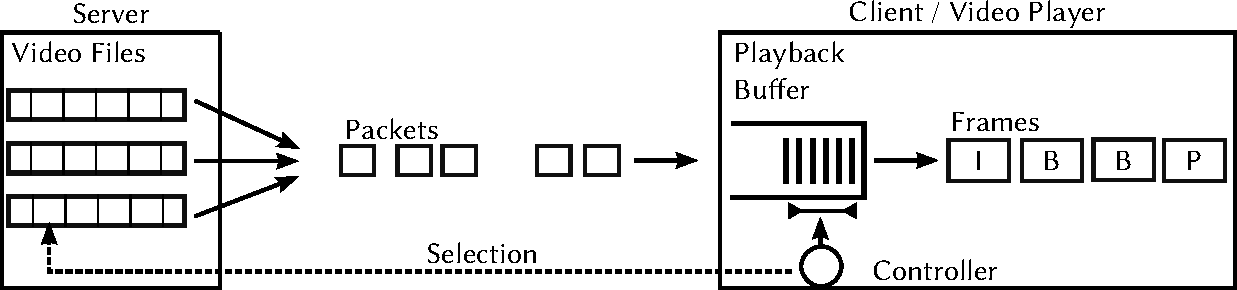
\includegraphics[width=0.9\textwidth]{images/playback-model.pdf}
    \caption{Reliable streaming playback model based on buffer control.}
    \label{c3:fig:playback-model}
\end{figure}

Figure~\ref{c3:fig:playback-model} overviews the reliable streaming model. The controller, part of the video player, selects a video from a remote location and the transmission is started, filling the playback buffer. The model has three degrees of freedom, which are all governed by the controller and together are coined playback strategies. These are:

\begin{itemize}
    \item The initial playback delay, which is the time between the initiation of the video stream transmission and the actual stream playback. The larger this is chosen, the bigger the safety margin on the buffer gets. If the video and transmission bitrate are known to be constant and and appropriately dimensioned, the initial delay can be chosen to be very small.
    \item Playback pause and resume decisions based on the current buffer fill level. This is a generalization of the initial playback delay, which is in fact only one, albeit always occurring stalling period.
    \item Selection of the video or video segment with a video bitrate chosen according to the current network throughput. This is only applicable for adaptive streaming.
\end{itemize}


These decisions yield a stalling period distribution for a streamed video. The frequency and the duration of stalls directly relate to the decision function of the playback model. The more frequent the stalls are, the shorter they will be; if the strategy produces longer stalls, they will be less frequent assuming the same network conditions. The time scale on which streaming applications buffer content usually lies in the range of seconds. This is a necessity in best-effort networks, as the available network bitrate might drop unexpectedly and cause stalling.


The the rest of this sections present fundamental playback strategies and strategy building blocks with features extracted from real world examples, which are given afterwards. 



%%
\subsubsection{Null Strategy}

The simplest strategy is having no strategy at all. Playback is started immediately when at least a single frame fully resides within the buffer and stops again at an empty buffer. The behavior can be summarized as ``Whenever anything can be played from the buffer, do so''.

This results in frequent stops and a large loss in playback continuity and will therefore not be used in practice. However, this strategy has some interesting theoretical properties, which is why it is mentioned here.
It minimizes total stalling time and the required buffer space. Moreover, it gives an upper limit for the number of stalls occurring\footnote{As a video frame is atomic, no other model could possibly stop the playback more often.}. Therefore, it can act as a baseline reference to assess the performance of other strategies.

\begin{figure}[htb]
    \centering
    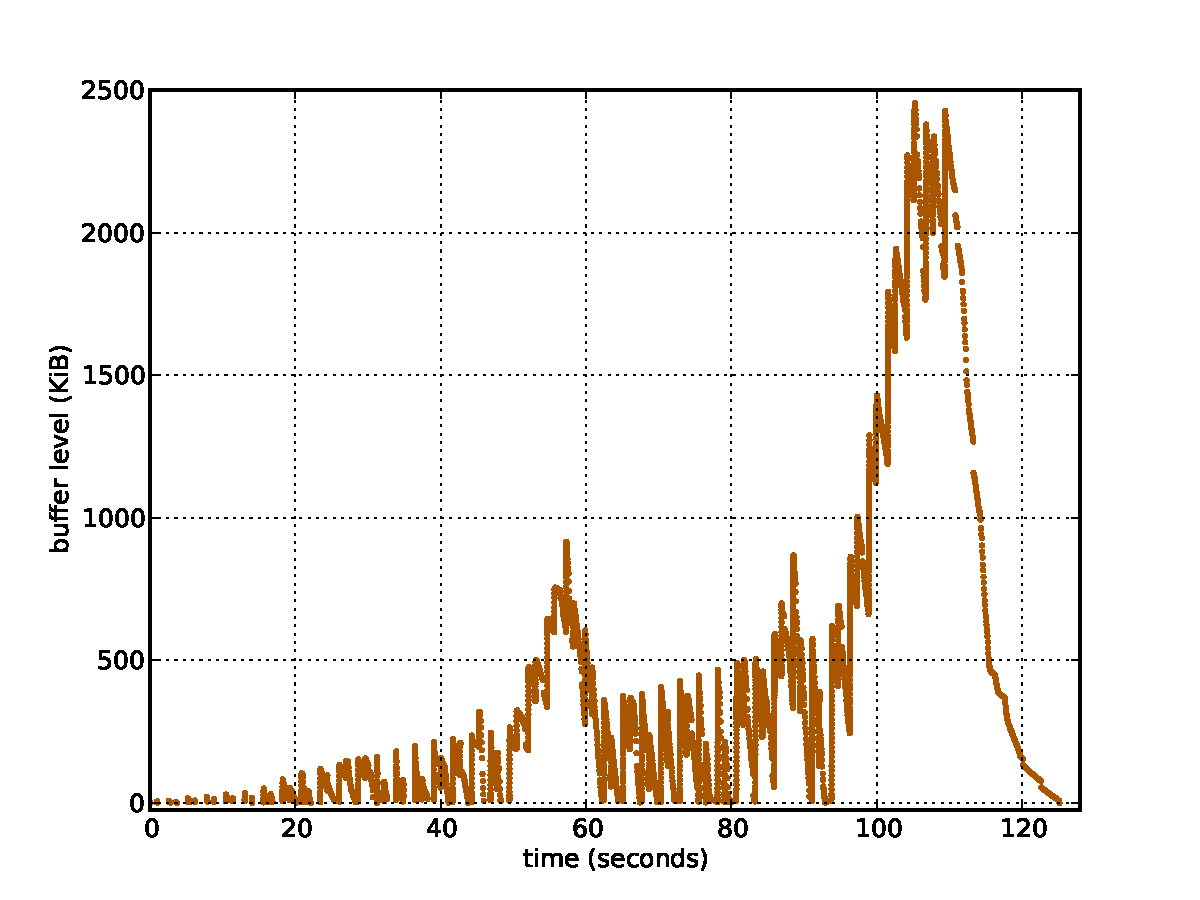
\includegraphics[width=0.9\textwidth]{images/bufferlevel-stall-new.pdf}
    \caption{Buffer fill level with null strategy; \SI{33}{\second} total stalling.}
    \label{c3:fig:bufferlevel-stall}
\end{figure}

Figure~\ref{c3:fig:bufferlevel-stall} depicts an exemplary time series diagram of the contents of a video buffer using this strategy with a transmission rate only slightly above the video stream's rate. The buffer frequently drops down to zero forcing a short stall. According to the presented related work on the \gls{QoE} impact of stalling frequency in comparison to the length of stalls \cite{6123395}, this is the worst possible scenario for a person watching the stream.


%%
\subsubsection{Threshold Strategies}

Instead of instantly restarting playback, a lower threshold can be introduced. Only after a certain buffer fill level threshold has been surpassed, playback will be started. Thresholds can be set independently for the initial playback delay and stalls, with the initial playback delay generally set to be higher.

The threshold can be chosen in a number of ways. It can either be an absolute data volume, a buffered video duration. The latter is much more suited for variable bitrate videos as it automatically adapts itself to the current bitrate. A third option is to buffer for a certain amount of real time -- this can be seen as threshold -- and starting playback after that period regardless of the volume of the buffer. Additionally, the threshold could also either be set to a constant value or dynamically chosen according to the expected network \gls{QoS}.

Besides this single-threshold strategy, a two-threshold strategy might make more sense for segment-based streaming. In addition to the lower threshold, an upper threshold is introduced. When reached, no new segments will be requested until the buffer arrives at the lower threshold again.  To achieve an hysteresis effect a third threshold, somewhere between the lower and upper bound, can also be introduced. Through this, the maximum buffer size can also be controlled. This is important in situations with hard limits on available memory. Mobile devices come to mind here.

\begin{figure}[htb]
    \centering
    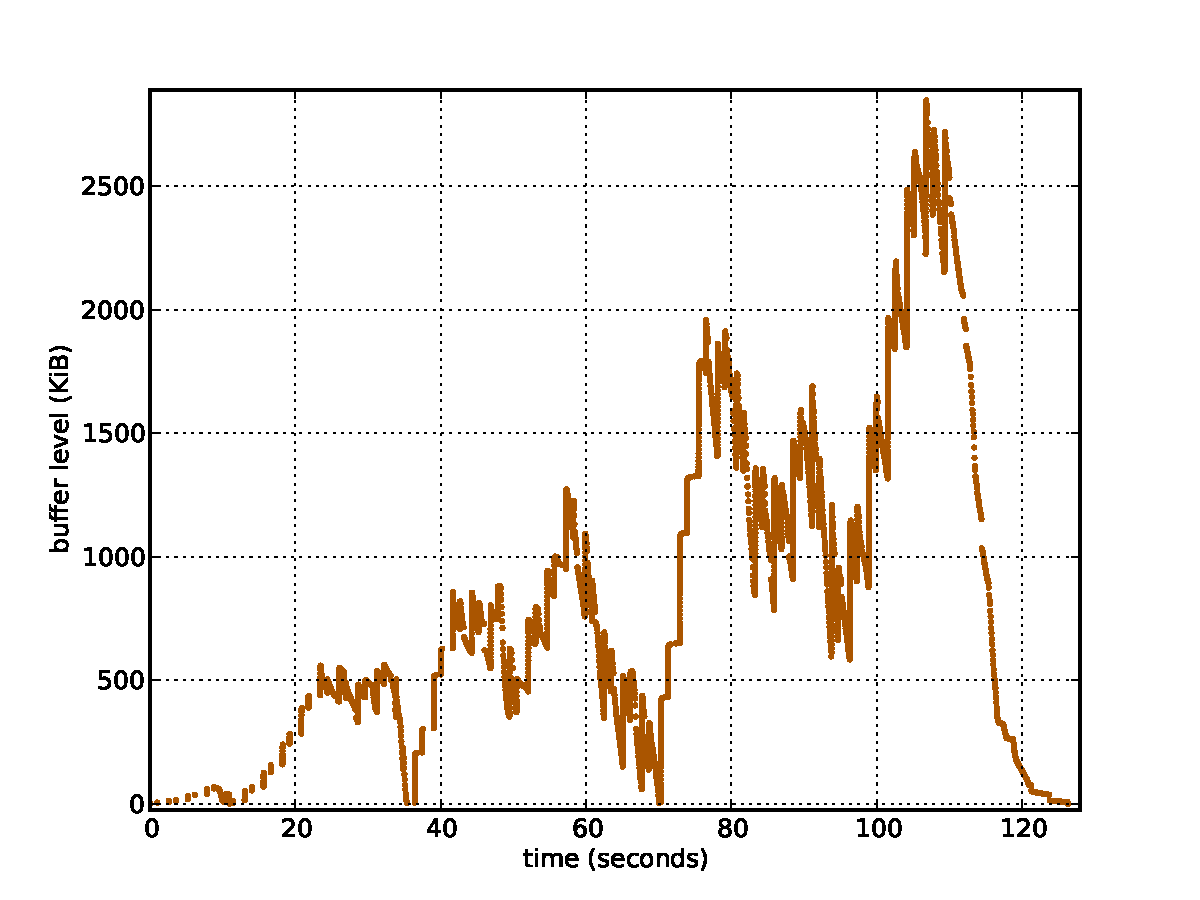
\includegraphics[width=0.9\textwidth]{images/bufferlevel-flash-new.pdf}
    \caption{Sample buffer fill level for a \SI{2}{\second} and \SI{5}{\second} buffered video duration threshold strategy; \SI{34}{\second} total stalling.}
    \label{c3:fig:bufferlevel-flash}
\end{figure}

An example buffer diagram is displayed in Figure~\ref{c3:fig:bufferlevel-flash}. In this case, the initial delay was controlled by a buffered video duration threshold of \SI{2}{\second} and a resume condition also based on buffered video duration but with a \SI{5}{\second} threshold. The strategy produces noticeable less stalls than the null strategy but slightly increases the total stalling time.


%%
\subsubsection{Pacing Strategies}

For segment-based \gls{HTTP} streaming, a two-threshold strategy is not the only supplemental option on top of simple streaming. Here, the controller can pace the request of future segments to match the overall, or the current video bitrate. A safety margin can also be factored in to even out short time fluctuations of either the transmission or the video bitrate. For example, the controller would request segments with an overall transmission rate of 1.25 times the video bitrate. The pacing rate can either be statically chosen in advance or can be calculated dynamically based on current or future conditions. The latter leads to predictive strategies.

%%
\subsubsection{Predictive Strategies}

In predictive strategies, knowledge of the future of the streaming process is used by the controller to adjust the start/stop and segment retrieval conditions. Instead of global knowledge, heuristics can instead attempt to approximate a future state.

A very simple predictive approach is to prolong the initial delay to the point, that no intermediate buffer underrun and thus no stall will occur. With global knowledge, the controller can start the stream at the earliest possible point in time, thus minimizing the total stalling time while still having only the initial delay.

\begin{figure}[htb]
    \centering
    \includegraphics[width=0.9\textwidth]{images/bufferlevel-startdelay-new.pdf}
    \caption{Sample Buffer fill level for the delayed playback model, \SI{33}{\second} total stalling.}
    \label{c3:fig:bufferlevel-startdelay}
\end{figure}

Figure~\ref{c3:fig:bufferlevel-startdelay} depicts the time series of a sample implementation of this delayed playback predictive strategy with all necessary stalling occurring upfront.


%%
\subsubsection{Adaptive Strategies}

Most strategies for adaptive streaming are an extension of both the threshold as well as the pacing strategy. However, instead of a simple transmit-or-no-transmit ruleset, they can make much more fine-grained adjustments. The quality of the stream segment to be requested will be chosen, depending on the current fill level and drain rate of the buffer. This makes a trade off between maintaining a certain quality level and putting up with increased waiting times, and dropping the quality to a level sustainable at the current transmission rate.


\subsubsection{Real World Implementation Examples}

Actual streaming player implementations often do not implement only one of these strategies, but rather combine ideas from several. Herein, thresholds are often set arbitrarily through the implementor's best practices and not empirically evaluated, often making a trade-off between user perceivable quality and resulting server load. In general, every streaming service practically implements its own playback strategies. This section describes three example applications.

%%
\paragraph{2011 YouTube Flash Player Buffering Strategy}

Google's video streaming site YouTube is constantly changing its appearance and technical makeup. In recent years, YouTube streams are delivered by one of three players: The Website's Flash player, a browser-integrated HTML5-based player, or custom player implementations in mobile phones, set-top boxes and similar devices. Here, the Flash-based variant used in 2011 is described.

This player used a single threshold strategy with different threshold values for the initial delay and any subsequent stalls. The values were already described in Figure~\ref{c3:fig:bufferlevel-flash}. This model assumes sufficient network conditions in the beginning, requiring only a short initial playback delay to pre-fill the playback buffer. If, however, stalling occurs, then it will buffer longer to keep the stalling frequency down.

\begin{table}[htb]
    % increase table row spacing, adjust to taste
    %\renewcommand{\arraystretch}{1.3}
    \caption{Transmission Related Parameters from YouTube's Video URL Setup}
    \label{c3:tbl:yturl}
    \centering
    \begin{tabu}{|X[l]|X[p]|}
        \hline
        URL Part & Description \\ \hline
        \texttt{v$\alpha$.lscache$\beta$.c.youtube.com} &  Cache server involved in the delivery.\\
        \texttt{algorithm=throttle-factor} and \texttt{burst=40} and \texttt{factor=1.25} & Indicates initial burst plus block sending configuration. \\
        \texttt{ratebypass=yes} & Parameter to indicate no rate limiting.\\ \hline
    \end{tabu}
\end{table}

Furthermore, YouTube employs a proprietary pacing mechanism outside of the control of the streaming player. This is hinted at in the encoding of the \glspl{URL} of the video files and enforced by the video file cache server. Some of those not user-changeable parameters are described in Table~\ref{c3:tbl:yturl}. The pacing was in effect for all videos below high definition resolution, but has since then been extended to include all video files. 

\begin{figure}[htbp]
% used yt-delay/hPUGNCIozp0_delay_100 2, spyder with matplotlib config patch
    \centering
        \begin{subfigure}[b]{0.90\textwidth}
                \centering
                \includegraphics[width=\textwidth]{images/blocktransfer-mod.pdf}
                \caption{Overall graph.}
                \label{c3:fig:blocktransfer-overall}
        \end{subfigure}

        \begin{subfigure}[b]{0.90\textwidth}
                \centering
                \includegraphics[width=\textwidth]{images/blocktransferdetail.pdf}
                \caption{Detail plot of the rate-limited block-sending phase.}
                \label{c3:fig:blocktransfer-detail}
        \end{subfigure}
\caption{Comparison of downloaded and consumed data volume revealing the pacing mechanism used by YouTube.}
\label{c3:fig:blocktransfer}
\end{figure}


The throttling method, also observed in \cite{alcock2011afcyt}, limits the transmission to a rate slightly above the average media bitrate, measurements and the \gls{URL} scheme indicates this to be a factor of the video bitrate of $1.25$. The rate limit is not constant, instead a ON-OFF block-sending scheme is facilitated. The scheme transmits short packet bursts, typically \SI{64}{\kibi\byte} in size, followed by long pauses as seen in Figure~\ref{c3:fig:blocktransfer}. The pause length between two bursts is set dynamically to reach the targeted bitrate on a larger time scale. The initial phase of the stream transmission is conducted unthrottled at line speed, presumably to allow for some pre-buffering to occur at the client media player. A possible reason for this server-side pacing is to avoid load spikes, with the added side effect of keeping the clients' buffer sizes in check.



%%
\paragraph{Firefox's HTML5 Player Strategy}

Video streaming can also be directly conducted with the Web browser, through the use of a HTML5 canvas element. The \gls{W3C} specifies the default technical process of HTMl5 video streaming in \cite{html5video} and essentially suggests a predictive strategy. Herein, the Web browser should estimate and correlate the transmission rate to the video bitrate. A property called ``autoplay'' uses this definition to start  playback of the associated video \enquote{as soon as it can do so without stopping}. The HTML5 strategy also allows to limit the buffer size through transmission pacing, negotiated with the server, and appropriately timed range requests.

The open-source Firefox browser represents an implementation of this specification and substantiates it further. The description of this strategy is based on Firefox's version 4.0 released in March 2011. Because it is an online algorithm which does not have global knowledge of the video and transmission speeds of any point in the future it has to estimate these.
To estimate the current and future rates, the moving average of the transmission rate $s_{MA}$ and the video bitrate $v_{MA}$ are calculated. The condition $c$ Firefox uses to start and resume the playback process is given in Algorithm~\ref{c3:alg:firefox}, with the buffered video duration $b_b$, and the duration spent buffering $b_T$.

\begin{algorithm}[htb]
    \centering
    \begin{algorithmic}
        \IF {$s_{MA} > v_{MA}$} 
          \STATE $c \gets ( b_b=20s \lor b_T=20s )$
        \ELSE
          \STATE $c \gets ( b_b=30s \lor b_T=30s )$
        \ENDIF 
    \end{algorithmic}
    \caption{Firefox playback (re-)start decision algorithm.}
    \label{c3:alg:firefox}
\end{algorithm}

 \begin{figure}[htb]
    \centering
    \includegraphics[width=0.9\textwidth]{images/bufferlevel-firefox-new.pdf}
    \caption{Sample buffer fill level for the Firefox 4 strategy, \SI{44}{\second} total stalling.}
    \label{c3:fig:bufferlevel-firefox}
\end{figure}


This approach is quite conservative and trades off long stalling periods for fewer stalls. The test case for our model is shown in Figure \ref{c3:fig:bufferlevel-firefox}. The playback starts only after a long waiting period and intermittent stalls cause a long buffering period. 
Due to the longer overall stalling time the player needs to buffer more data than other strategies. This may make it unsuitable for devices with sparse amounts of memory, e.g. mobile phones. On the other hand, could a large buffer also increase the chance of continuous playback in such scenarios with bad \gls{QoS}.


\paragraph{Adaptive streaming strategies}

Implementations for adaptive streaming players are again mostly proprietary and their behavior has to be derived from measurements. This is even true for adaptive streaming protocols, which have open specifications as these generally do not specify the player's behavior.

Microsoft's Silverlight player's strategy is described in \cite{BLTJ:BLTJ20505}. It employs a two-threshold model and rate estimations. When on of the thresholds is reached, the quality will be adjusted by one step upwards or downwards as long as the transmission rate is sufficient.

The buffering behavior of further protocol variants, including Adobe's \gls{HTTP} Dynamic Streaming, Apple's \gls{HTTP} Live Streaming and a sample implementation of \gls{DASH}, are investigated in \cite{Muller:2012:EDA:2151677.2151686,akhshabi2011experimental}.




% \begin{itemize}
% \item The player has been buffering data for at least 30 seconds.
% \item The player has already buffered an amount of data corresponding to 30 seconds of video.
% \item The video download has been completed.
% \item The moving average of the transmission rate is larger than the moving average of the video bitrate and the player has a safety buffer with 20 seconds of video data.
% \end{itemize}

% \begin{table}[htb]
%     \caption{Variables involved in buffering decisions.}
%     \label{c3:tbl:buffvars}
%     \centering
%     \begin{tabu}{|l|X[p]|} 
%     \hline
%     Variable & Description \\ \hline
%     $s_{MA}$ & Moving average of the transmission speed. \\
%     $v_{MA}$ & Moving average of the video bitrate. \\ 
%     $c$   & Condition upon which to start/resume playback. \\
%     $b_b$    & Amount of video data the buffer contains. \\
%     $b_T$    & Amount of time spent in non-playing buffering state. \\ \hline
%     \end{tabu}
% \end{table}

% used yt-delay/hPUGNCIozp0_delay_2500 1, spyder, color #aa5500
% data
% start delay 33s 
% flash 33.82s
% stalling 32.68s
% html5 as implemented in firefox 44s


%Which offers better quality to users? Some approaches (TODO: refs and explain how)

% Longer waiting time but very few stops. Stalling model definitely the shortest waiting time but stops too frequent with insufficient network conditions, i.e. can not really be used. Delayed playback requires total knowledge not available beforehand. Can maybe used with reduced information, bandwidth estimation, but this is essentially HTML5/Firefox.




%``application comfort'' time to skip, ...
%\subsubsection{Unreliable Streaming Metrics}
%... and why they mostly do not work / are not applicable.


%%%%%%%%%%%%%%%%%%%%%%%%%%%%%%%%%%%%%%%%%%%%%%%%%%%%%%%%%%%%%%%%%%%%%%%%%%%%%%%%
%!TEX root = ../../dissertation.tex
%%%%%%%%%%%%%%%%%%%%%%%%%%%%%%%%%%%%%%%%%%%%%%%%%%%%%%%%%%%%%%%%%%%%%%%%%%%%%%%
\section{Load Model Queuing Simulation} 
\label{c4:sec:simulation}

As discussed, the solvability of a non-stationary Erlang loss system is very limited. To better tackle this, a simulative approach can be taken. Depending on the level of detail, different types of simulations are available.

Here, a queuing simulation is used to ascertain the blocking probability and tunnel serving slot utilization from the model using the fitted distributions from the trace.


%%%%%%%%%%%%%%%%%%%%%%%%%%%%%%%%%%%%%%%%%%%%%%%%%%%%%%%%%%%%%%%%%%%%%%%%%%%%%%%
\subsection{Queuing Simulation Implementation}

The queuing simulation is implemented on the basis of a \gls{DES}. Instead of reproducing continuous time, this simulation is a series of discrete events. Time is advanced only at these events. 

A queuing model can be easily represented in a \gls{DES}.  Each tunnel request arrival is modeled as a discrete event. When such an event occurs, three processes are executed. The first process draws a random number from a \gls{PRNG} mapped to \gls{IAT} exponential distribution to schedule the next arrival event. Secondly, the serving units are checked for any free units. If one is found, it will now be occupied. Else, this arrival will be marked as rejected and the third action skipped. This third process now determines the length of the tunnel using another \gls{PRNG} adjusted to the serving time distribution to schedule the event in which the tunnel exits the system.

This model was implemented on the basis of version 3.0 of the \textit{SimPy}\footnote{\url{https://simpy.readthedocs.org/}} package, which is a Python \gls{DES} framework that provides the basic event and scheduling infrastructure. On top of this a base \gls{GGSN} class was constructed, managing the arrival of tunnel events and the scheduling of the service ending events. Specific classes for the traditional (i.e. monolithic) and virtualized (called ``multiserver'' in the code) nodes respectively exist.\footnote{The implementation is also publicly available at \url{https://github.com/fmetzger/ggsn-simulation/} as a reference.}


%%%%%%%%%%%%%%%%%%%%%%%%%%%%%%%%%%%%%%%%%%%%%%%%%%%%%%%%%%%%%%%%%%%%%%%%%%%%%%%
\subsection{Description and Design of the Individual Experiments}

To match the measurement data the simulation time is set to be \SI{7}{\day} in all simulation scenarios. The initial \SI{60}{\minute} of each experiment are considered to be the transient phase and are afterwards deducted from the results. Ten replications of each scenario were performed. All depicted error bars show the \SI{95}{\percent} confidence intervals across the experiments.

The first experiment was conducted to investigate the normalized baseline load a monolithic \gls{GGSN} experiences using the presented model. Using this, a maximum to the number of concurrent tunnels and the correlation to the blocking probability and tunnel rejection rate can be established. The effects of scaling up, improving the hardware capabilities of the single node, can thus be investigated.

Based on these results, the virtualization and scaling out effects in the virtualized, \gls{GGSN} model are examined. In order to study the feasibility of this approach the performance indicators of the virtual \gls{GGSN} are compared to the baseline established in the first experiment. To this end, the virtual \gls{GGSN} is simulated in configurations varying the number of instances and supported concurrent tunnels per instance.

In a final experiment the startup and shutdown duration of virtual instances and the life cycle management of these instances are additionally taken into account. Although the boot duration of modern \glspl{os} and \glspl{VM}, especially on current hardware with flash storage, is significantly lower than it has been in the past, there is still a delay. This could cause further blocking if the load balancer does not account for this. But the more generously the balancer starts instances in advance the smaller the virtualization efficiency gain, especially the energy consumption, will be become. For this reason, the number of active instance is a relevant performance metric in the virtual \gls{GGSN} model.

The experiment varies the boot delay and implements a very simple load balancer rule as baseline. The rule keeps at least one empty instance running in reserve at all times and deactivates instances, when two running instances are completely unused. As this is very generous, virtualization blocking should only occur in cases of very small instances or very rapid arrivals. Realistic provisioning rules can improve on this quite easily. But even this simplistic approach already serves to demonstrate potential benefits.


%%
\subsubsection{GGSN Load, Capacity, and Scaling}

First, with the help of the \glspl{IAT} and duration of tunnels calculated in the dataset evaluation, the monolithic \gls{GGSN} model is studied. While these traces provided information on the frequency of new tunnels and the duration they remain active, no reliable information on the number of required supported concurrent tunnels for a given arrival rate could be deduced. 
This experiment evaluates arbitrary values for the \gls{GGSN} tunnel capacity and determines the resulting blocking probability such that a suitable value can be found. This is a typical task in a dimensioning process.

\begin{figure}[htb]
	\centering
	\includegraphics[width=0.9\textwidth]{images/R-monolithic-blocking.pdf}
	\caption{Impact of the number of supported parallel tunnels on the blocking probability for the traditional \gls{GGSN} model. For each scenario the mean and \SI{95}{\percent} confidence intervals of all simulation replications are shown.}
\label{c4:fig:traditional_blocking}
\end{figure}

Figure~\ref{c4:fig:traditional_blocking} studies this impact of the maximum supported number of concurrent tunnels $n$ on the blocking probability $p_B$. $n$ is incrementally increased in steps of \numprint{100} tunnels from \numprint{0} to \numprint{5500}. As expected, the blocking probability decreases with the number of supported tunnels. An almost linear correlation can be observed in the larger part of the graph with a small convergence phase shortly before reaching $p_B=0$. For the normalized inter-arrival no blocking is occurring if a capacity of \numprint{5000} concurrent tunnels is allocated to the \gls{GGSN}.

\begin{figure}[htb]
	\centering
	\includegraphics[width=0.9\textwidth]{images/R-monolithic-tunnelusage.pdf}
	\caption{Mean number of tunnels concurrently served by the \gls{GGSN} for incrementally increasing capacity. For each scenario the mean and \SI{95}{\percent} confidence intervals of all simulation replications are shown.}
\label{c4:fig:traditional_tunnelusage}
\end{figure}

A similar picture is also evident in the number of tunnels served by this \gls{GGSN} in the same scenario as shown in Figure~\ref{c4:fig:traditional_tunnelusage}. For the first half of the experiments the \gls{GGSN} is loaded to its limit. Only when the capacity reaches \numprint{4600} can the normalized arrival rate be fully served, which surmounts to about \numprint{3820} tunnels on average in the system. Both results are stable across all simulation runs as the confidence intervals display. For the purpose of network dimensioning the results can be easily scaled up from the normalized arrival rates to the actual ones in the network in question.


%%
\subsubsection{Virtualization Impact and Gain}

A similar experiment can be set up for the virtual \gls{GGSN} model. Learning from the monolithic model, these follow-up simulations can be tuned to the same total tunnel capacity in advance. The only difference is that the tunnel capacity is now spread out evenly between the virtual \gls{GGSN} instances. The experiment tests different amounts for the total number of virtual instances, ranging from \numprint{1}, which represents the monolithic architecture, up to \numprint{100} instances in steps of \numprint{10}.

\begin{figure}[htb]
	\centering
	\includegraphics[width=0.9\textwidth]{images/R-virtualized-blocking.pdf}
	\caption{Comparison of the mean blocking probability of various server configurations with \SI{95}{\percent} confidence intervals. The x axis depicts the summary capacity of all virtual instances in the experiment.}
\label{c4:fig:virtualized_blocking}
\end{figure}

\begin{figure}[htb]
	\centering
	\includegraphics[width=0.9\textwidth]{images/R-virtualized-tunnelusage.pdf}
	\caption{Comparison of the mean tunnel occupation of various virtualization configurations with \SI{95}{\percent} confidence intervals.}
\label{c4:fig:virtualized_tunnelusage}
\end{figure}

Figures~\ref{c4:fig:virtualized_blocking} and \ref{c4:fig:virtualized_tunnelusage} demonstrate the results in terms of $p_b$ and concurrent tunnels served overlaid onto the base monolithic scenario's results. No large difference in the results can be seen and the virtualized \gls{GGSN} model behaves no worse than a single large node model.

\begin{figure}[htb]
	\centering
	\includegraphics[width=0.9\textwidth]{images/R-virtualized-mean-instanceusage.pdf}
	\caption{Mean instance usage of various virtualization configurations. A higher number of total instances results in a finer granularity of scaling and energy efficiency as more instances can be kept shut down.}
 \label{c4:fig:res-instance-usage-mean}
\end{figure}

But the possible effects of an increased number of instances need to be investigated further. One goal in virtualization is the increase of energy efficiency. This can be achieved by having turned on just as many instances as needed and not more, thus scaling the system to its current load. 

Therefore, Figure~\ref{c4:fig:res-instance-usage-mean} takes a look at scenarios with nine different instance pools and varying tunnel capacities for each instance. Each setup is compared by the mean number of active instances during the one-week course. The bigger the instances' capacity becomes the less instances need to be active. An actual \gls{GGSN}, even a virtualized one, would need to be dimensioned in such a way to keep the total overhead low. It was already determined that, with the assumed normalized arrival rate, a capacity of \numprint{5000} tunnels is sufficient in order to achieve a blocking probability close to zero. Keeping the setup at this minimum capacity and taking a look at the results in the figure, a good portion of the instances, usually around \SI{20}{\percent}, can still be kept turned off.

\begin{figure}[htb]
	\centering
	\includegraphics[width=0.9\textwidth]{images/R-virtualized-instanceuse.pdf}
	\caption{Impact of the maximum number of tunnels and number of instances on the number of active instances in the virtual \gls{GGSN} model.}
\label{c4:fig:virtualized_instanceuse}
\end{figure}

To get into more detail, Figure~\ref{c4:fig:virtualized_instanceuse} displays the distribution of the portion of time a specific number of instances was active. Depicted are four configurations that differ in their total number of instances and their tunnel capacity. The setup with \numprint{30} instances with \numprint{100} capacity was clearly overwhelmed with the arrival rate and all \numprint{30} instances were active over \SI{70}{\percent} of the time. Only when \numprint{150} were allowed the virtualization benefits come into effect and more instances are able to sleep. Similar observations can be made in the \numprint{50} instance case.  Here, the \numprint{100} tunnel scenario is already equipped to handle the tunnel arrival rate and can scale back its active instances quite well, below \numprint{40} instances half the time. The final configuration with a \numprint{150} tunnel capacity is clearly overdimensioned here with no more than \numprint{33} of the \numprint{50} instances ever being active.

\begin{figure}[htb]
	\centering
	\includegraphics[width=0.9\textwidth]{images/R-virtualized-instanceuse-barplot.pdf}
	\caption{Resource usage from a select maximum instances and tunnel capacity combination, displaying the capability to scale up and out.}
\label{c4:fig:res-usage-barplot}
\end{figure}


Looking at these scenarios and additionally Figure~\ref{c4:fig:res-usage-barplot} from a network dimensioning perspective, two distinct pathways to scale in the virtualized \gls{GGSN} model are revealed. To reach the desired tunnel capacity either the number of instances or the instance's tunnel capacity can be increased. The latter represents the classical \textit{scaling up}. But virtualization also opens up the new path of \textit{scaling out} by increasing the number of instances. Through this, scaling can be become easier and cheaper as existing machines need not be replaced any more.


%%
\subsubsection{Virtual Instance Life Cycle Management Impact}

A final aspect to be investigated in the experiments is the potential increase of the blocking probability in virtualized scenarios when compared to the monolithic base. In theory, virtualization can incur additional overhead which would represent itself as an increase in $p_b$. In the given model the overhead can stem from the hypervisor and its scheduling  and lifecycle management strategies in conjunction with the instances' boot delay. 

The somewhat simplistic hypervisor strategy in this simulation was already discussed above and should give an upper limit on the impact on the blocking probability. This strategy is fixed, but the instance boot duration gets changed to analyze the impact. Values between \SI{20}{\second} and \SI{5}{\minute} are considered and should reasonable represent real-life systems of a wide variety.

\begin{figure}[htb]
	\centering
	\includegraphics[width=0.9\textwidth]{images/R-virtualized-startstop-blocking-barchart.pdf}
	\caption{Influence of the boot and shutdown time on the blocking probability.}
\label{c4:fig:blockprob-startstop-barchart}
\end{figure}

Figure~\ref{c4:fig:blockprob-startstop-barchart} compares a number of instance and tunnel capacity scenarios on basis of their instance boot duration. In most scenarios there is almost no increase in the tunnel blocking probability. Only in cases with very many but small instances, where a lot of instance churn will occur, an increase can be noticed for higher boot durations.

\begin{figure}[htb]
	\centering
	\includegraphics[width=0.9\textwidth]{images/compare-maxinstances-block.pdf}
	\caption{Influence of start up and shut down time on blocking probability with regard to different numbers of instances.}
\label{c4:fig:compare_maxinstances_block}
\end{figure}

Figure~\ref{c4:fig:compare_maxinstances_block} investigates this increase in more detail and shows the blocking probability of one select scenario. Here, the system supports \numprint{5000} tunnels in total with differing individual instance capacity of \numprint{50}, \numprint{150}, and \numprint{500}. In each case the start and stop down duration is changed between \SI{1}{\minute} and \SI{5}{\minute}. The increase in blocking probability in relation to both the instance capacity as well as the start duration can be easily observed.

This can be partially attributed to the hypervisor and its simplistic scheduling  and lifecycle management strategies in the simulation. If a low capacity instance with a long start time is activated, there is a high probability that the system will quickly expend its capacity again.
A potential conclusion is that choosing larger instance capacities decreases the blocking probability at the cost of energy efficiency (because less instances can stay turned off).

\begin{figure}[htb]
	\centering
	\includegraphics[width=0.9\textwidth]{images/R-virtualized-startstop-tunnelusage-blocking-comparison.pdf}
	\caption{Trade-off between blocking probability and mean resource utilization with regard to maximum number of instances, instance tunnel capacity, and start and stop time.}
\label{c4:fig:compare_util_block}
\end{figure}

Finally, Figure~\ref{c4:fig:compare_util_block} shows two scenarios with \numprint{40} and \numprint{100} virtual \gls{GGSN} instances respectively, and \numprint{1000} to \numprint{5000} total concurrent tunnels. For each scenario, the combined impact of different individual instance tunnel capacities as well as start up and shutdown time on blocking probability and mean resource utilization is studied. The first observation is that by increasing the number of instances, i.e., scaling out, the blocking probability can be decreased, while maintaining a relatively low mean resource utilization. 

In addition to the previous effects, it can be noticed that a higher start up and shut down time causes a slight increase in blocking probability for instances with low tunnel capacity. Therefore, if smaller instances are to be used, for example due to price considerations, both the start up and shut down duration should be kept at a minimum. This could be achieved by using purely virtual instances and fast flash storage.


%%
\subsubsection{Significance and Effect Sizes}

In order to analyze the influence of the different model parameters on the resulting metrics a one-way \gls{ANOVA} is performed. The effect size measures calculated here are the F-test, $\eta^2$, as well as $\omega^2$~\cite{stats,field2012discovering}. All are applied pairwise to each independent and derived variable combination. The results are depicted in Table~\ref{c4:tab:anova}. The two derived values and simulation metrics are the blocking probability and the mean tunnel usage.

\begin{table}[htb]
\caption{Effect sizes of the simulation parameters based on a one-way \acrshort{ANOVA}.}
\label{c4:tab:anova}
	\centering
	\begin{tabu}{X[2.5,l]X[1.0,r]X[0.6,r]X[0.6,r]X[0.6r]}
	\toprule
	& $\mathbf{F-ratio}$ & $\mathbf{p-value}$ & $\mathbf{\eta^2}$ & $\mathbf{{\omega}^2}$\\ 
	\midrule
	\multicolumn{2}{c}{\textbf{Blocking probability}} & & & \\ 
	Individual instance tunnel capacity & $104$ & $<0.001$ & $0.468$ & $0.463$\\ %F(12, 1417)=
	Number of instances & $9.29$ & $<0.001$ & $0.056$ & $0.050$\\ %F(9,1420)=
	Start/stop duration & $0.21$ & $0.931$ & $<0.001$ & $0.002$\\ %F(4,1425)=
	Total tunnel capacity & $317257$ & $<0.001$ & $0.999$ & $0.999$ \\ %F(12,1417=
	\midrule
	\multicolumn{2}{c}{\textbf{Mean number of tunnels}}& & & \\ 
	Individual instance tunnel capacity & $105.7$ & $<0.001$ & $0.472$ & $0.467$\\ %F(12,1417)=
	Number of instances & $9.39$ & $<0.001$ & $0.056$ & $0.050$\\ %F(9,1420)=
	Start/stop duration & $0.25$ & $0.912$ & $<0.001$ & $0.002$\\ %F(4,1425)=
	Total tunnel capacity & $365753$ & $<0.001$ & $0.999$ & $0.999$ \\ %F(12,1417)=
	\bottomrule
	\end{tabu}
\end{table}

Both of these metrics yield very similar results as they are also --- by design --- strongly related to each other. The F-ratio computed by the F-test and the corresponding significance level $p$ indicate a large influence of the individual instance capacity on the metrics with a minor influence of the number of instances and no measurable impact of the start/stop duration. This is also confirmed by both $\eta^2$ and $\omega^2$. Interestingly, only the compound variable describing the total tunnel capacity, i.e., the product of the individual instance tunnel capacity and the number of instances, is an almost perfect match in its variance to the derived metrics.




%https://www.msu.edu/~levinet/eta%20squared%20hcr.pdf
% https://en.wikipedia.org/wiki/F-test
% F(2,1275): degrees of freedom (DF) for boh variables
% F-ratio: ratio of the model to its error; Note F(x, y) denotes an F-distribution with x degrees of freedom in the numerator and y degrees of freedom in the denominator.
% eta-squared, omega-squared, f-squared and effect sizes: https://en.wikiversity.org/wiki/Effect_size , https://en.wikipedia.org/wiki/Effect_size
% see also: https://en.wikipedia.org/wiki/Manipulation_checks

% Cohen's f is an effect size measure.  It is handy for power analysis as Cohen describes in "Statistical Power Analysis for the Behavioral Sciences."
% It is a "pure number to index the degree of departure from no effect."  
%The computation/use of f depends on the type of analysis used; fixed effects are an assumption (p. 273).  Cohen indeed gives f as f = (sqrt(eta^2 / (1 - eta^2)) for one-way fixed factor designs.  Since "there is no need to adjust one's conception of f for a set of k means when one moves from the one-way ANOVA to the case where additional bases of partitioning of the data exists," there doesn't seem to be any computational difference across the ANOVA designs. 

% https://en.wikiversity.org/wiki/Eta-squared

% https://stats.stackexchange.com/questions/15958/how-to-interpret-and-report-eta-squared-partial-eta-squared-in-statistically




% \begin{table}[htb]
%   \caption{Effect sizes of the simulation parameters based on one-way \acrshort{ANOVA}.}
%   \centering
%   \label{c4:tab:manipulation2color}
%   \begin{tabu}{X[1.6,l]X[r]X[r]X[r]X[1.1r]X[1.1,r]}
%   \toprule
%   & $\mathbf{F(2,1275)}$ & $\mathbf{\eta^2_p}$ & $\mathbf{p}$ & \textbf{Cohen's} $\mathbf{f^2}$ & \textbf{Cohen's} $\mathbf{\hat{\omega}^2}$\\ 
%   \midrule
%   \multicolumn{2}{l}{\textit{blocking probability}} & & & &\\ 
%   maxTunnels &  $15601.534$ & $\color{red}0.99$ & $<0.001$ & $\color{red} 26.739$ & $0.964$\\ 
%   maxInstances &  $10218.173$ & $\color{red} 0.986$ & $<0.001$ & $\color{red} 1.068$ & $0.516$\\ 
%   startstopDuration & $0.868$ & $\color{black} 0.003$ & $0.482$ & $\color{black} 0.000$ & $0.000$\\
%   \midrule
%   \multicolumn{2}{l}{\textit{mean number of tunnels}}& & & &\\ 
%   maxTunnels & $20448.347$ & $\color{red} 0.994$ & $<0.001$ & $\color{red} 27.712$ & $0.965$\\ 
%   maxInstances & $13348.251$ & $\color{red} 0.989$ & $<0.001$ & $\color{red} 1.064$ & $0.515$\\ 
%   startstopDuration & $2.872$ & $\color{black} 0.009$ & $0.022$ & $\color{black} 0.000$ & $0.000$\\
%   \bottomrule
%   \end{tabu}
% \end{table}



% \begin{figure}[htb]
%   \centering
%   \includegraphics[width=1.0\textwidth]{images/blocking-comparison.pdf}
%   \caption{Relative increase of blocking probability on the number of servers compared to the traditional \gls{GGSN}; with the $4500$ maximum tunnels per server being on a single server, $150$ on $30$, and $75$ on $60$ servers.}
% \label{c4:fig:blocking-comparison}
% \end{figure}

%%%%%%%%%%%%%%%%%%%%%%%%%%%%%%%%%%%%%%%%%%%%%%%%%%%%%%%%%%%%%%%%%%%%%%%%%%%%%%%%
\section{Core Network Summary}
\label{c4:sec:conclusion}

This chapter gave a broad overview of the \gls{3G} mobile core network control plane and attempts to determine a fitting definition for control plane load. This can not be achieved without first understanding many of the aspects and protocols unique to mobile networks. And these differ a lot from the conventional wisdom found in wired network architectures. With this knowledge at hand, a week long measurement trace acquired in the core network of an Austrian mobile operator was investigated. 

The control plane load definition serves as an essential distinction to regular mobile network investigations, which usually consider just the user plane. Concluding from the trace, the investigation of \gls{gtp} tunnel properties was determined to be a worthwhile measure for control plane load at the \gls{GGSN}, one of the central nodes in a \gls{3G} core network.

The investigation also showed, that the control plane is easily influenced by several device-based --- as far as they can be distinguished in a core network trace --- and time-of-day related features. The overall diurnal tunnel signaling load closely resembles the progression of the user plane. Most of the control plane's procedures are still triggered, either directly or indirectly, by user devices, of which the offered load is much smaller during night time. The trace evaluation also confirms the dominating influence of smartphones compared to other devices types, even when looking at the control plane.

But this also means, that sheer traffic volume is not a good measure to determine load, as the per-device traffic volume of a smartphone is rather low when compared to devices like pure \gls{3G} modems attached to a notebook. In this aspect, the findings also support the stories of signaling storms in mobile networks caused by applications regularly causing small amounts of network traffic. Each application interaction results in disproportionate amounts of signaling load being generated. Even worse, measures taken to improve the radio interface control plane such as Fast Dormancy could possibly have adverse effects to core signaling as they might increase the tunnel churn.

But the load investigation should not stop here. The presented approaches were just the ones that could be conducted with the available data. If one were to have access to a mobile network monitoring system or more detailed data records from such a system, it would open up many more angles in the investigation. For example, recording every individual signaling message with all \glspl{IE} would give hard numbers on the direct signaling overhead, as could measurement probes located inside the network nodes report on the CPU and memory load in order to determine the control plane's processing overhead. A closer investigation of control plane load in relation to mobility behavior should also prove very interesting, as this is one of the central motifs in every mobile network.

Learning from this historical data, queuing theoretic models were created that can describe the control plane load in such networks. These models can be easily used in network dimensioning and planning processes by means of, e.g., stationary analyses. The novel baseline control plane load model presented here is a $M(t)/G(t)/c/0$ non-stationary Erlang loss model. When used in conjunction with parameters derived from the measurement traces it can easily be used for network dimensioning. To improve scaling in the future a further \gls{GGSN} load model with features used in virtualization was also proposed.

Due to general solvability issues of non-stationary Erlang models the model is evaluated and validated using a queuing simulation in terms of their blocking and tunnel state probability as well as the general resource utilization. The virtual model provided the added benefit of being more flexible in its scaling properties and energy efficiency. This might even lead to new \gls{GGSN}-as-a-Service business models, removing the need to provide and operate large amounts of infrastructure for rare cases of peak load. 

%In the future we would like to deepen our modeling efforts to provide more dimensioning options for a core network. Also, we want to further investigate the correlation of user traffic and signaling and take a look at the implications specific traffic types bring for the core network. 

%All these investigations and modeling efforts combined could lead to a more informed approach of network planning: Being more aware of the control plane provides the necessary tools to identify probable causes for control plane activity. 

%We would also like to expand our evaluations, as there are several angles not investigated so far that could prove worthwhile. This includes an examination of the exact number and size of signaling messages flowing through the core, a more detailed picture of the processing load these messages induce at the \gls{GGSN}, and an evolved model. Furthermore, a differential analysis of our data compared to a newer dataset (potentially including \gls{LTE} access) could really prove worthwhile.

%We also look forward to searching for multiple active tunnels per device. As discussed previously, the \textit{Secondary PDP Context Activation Procedure} enables devices to establish up to ten additional tunnels attributed with a different, higher QoS level, if the network supports this. The additional load of managing and holding multiple tunnels plus the displacement of other, ``lower-quality'' traffic could prove to be an interesting investigation. Initial observations indicate that this feature is rarely used today by very few types of devices, but it will be of increased interest in the face of ongoing LTE/EPS deployments, whose specifications expand upon this secondary tunnel concept.